\documentclass{article}

\usepackage{metalogo}
\usepackage{geometry}
\usepackage{indentfirst}
\usepackage{graphicx}
\usepackage{array}
\usepackage{booktabs}
\usepackage{listings}
\usepackage{color}
\usepackage{float}
\usepackage{tikz}
\usetikzlibrary{shapes.geometric, arrows, positioning, calc}
\usepackage{textcomp}
\usepackage{chngcntr}
\usepackage{enumerate}
\usepackage{fancyhdr}
\usepackage{multirow}
\usepackage{multicol}
\usepackage[colorlinks=false, pdfborder=0 0 0, bookmarksopen=true]{hyperref}
\usepackage{bookmark}
%\usepackage[backend=biber, style=numeric]{biblatex}
\usepackage[perpage]{footmisc}
\usepackage{setspace}
\usepackage{longtable}
\usepackage{arydshln}
\usepackage{amssymb}
\usepackage{amsmath}
\usepackage[thinlines]{easytable}
\usepackage{tocloft}
%\addbibresource{./citation.bib}		% the References, run xelatex, biber *.bcf, xelatex, xelatex

%% Ctex settings %%%%%%%%
%%%%%%%%%%%%%%%%%%%%%%%%%
\usepackage[
fontset=none,		% a must-have option
heading=true,		% <true|false>		enable heading, affecet numbering
scheme=chinese,		% <chinese|plain>	use chinese scheme
linespread=1.3,		% line spreading
zihao=5				% set font size
]{ctex}

% this is an workaround for the wrong hyperref content
\newlength{\tempspacewidth}
\setlength{\tempspacewidth}{3em}

\ctexset{
	fontset=adobe,				% <adobe|fandol|founder|ubuntu|mac|windos|windowsnew|...>
	punct=quanjiao,				% <quanjian|banjiao|kaiming|plain>
	autoindent=true,			% <true|false|num|num-with-metric>
	today=small,				% <small|big|old> old for English format
	contentsname=目录,			% name of the content
	listfigurename=插图,		% name of listfigure
	listtablename=表格,			% name of the list table
	figurename=图,				% name of the figure
	tablename=表,				% name of the table
	indexname=索引,				% name of the index
	appendixname=附录,			% name of the appendix
	% --------------------------------------------
	% Whether parts's header should be numbered -- Number
	part/numbering=true,
	section/numbering=true,
	subsection/numbering=true,
	subsubsection/numbering=true,
	paragraph/numbering=true,
	subparagraph/numbering=true,
	appendix/numbering=true,
	% --------------------------------------------
	% Control the format of the NUMBERIG --------- Number
	part/name={实验,},
	section/name={,},					% section name, has the format of {AAA,BBB}
	subsection/name={,},
	subsubsection/name={,},
	appendix/name={附录},
	section/number=\Roman{section},		% can use \chinese{<counter>}
	subsection/number=\Roman{section}.\arabic{subsection},
	subsubsection/number=\Roman{section}.\arabic{subsection}.\arabic{subsubsection},
	paragraph/number=\arabic{paragraph},
	subparagraph/number=\arabic{paragraph}.\arabic{subparagraph},
	appendix/number=\Alph{section},
	% --------------------------------------------
	% Control the format of parts' header -------- Global
	part/format=\centering\LARGE\bfseries,
	section/format=\flushleft\Large\bfseries,		% add \centering here if you want to centralize it
	subsection/format=\flushleft\large\bfseries,
	subsubsection/format=\flushleft\normalsize\bfseries,
	paragraph/format=\flushleft\normalsize\bfseries,
	subparagraph/format=\flushleft\normalsize\bfseries,
	% --------------------------------------------
	% Control the format of TOC ------------------ Name
	part/tocline=\LARGE\bfseries\CTEXnumberline{#1}#2,
	section/tocline=\Large\bfseries\CTEXnumberline{#1}#2,		% \CTEXnumberline means that if the section/etc has no name, then do not output the num
	subsection/tocline=\large\bfseries\CTEXnumberline{#1}#2,
	subsubsection/tocline=\normalsize\bfseries\CTEXnumberline{#1}#2,
	paragraph/tocline=\normalsize\CTEXnumberline{#1}#2,
	subparagraph/tocline=\normalsize\CTEXnumberline{#1}#2,
}


%% settings %%%%%%%%%%%%%
%%%%%%%%%%%%%%%%%%%%%%%%%
\geometry{left=1.25in, right=1.25in, top=1in, bottom=1in}
\lstset{language=[x86masm]Assembler,
		tabsize=4,
		breaklines=true,
		frame=shadowbox,
		framexleftmargin=7mm,
		rulesepcolor=\color{black},
		basicstyle=\footnotesize,
		numbers=left,
		showspaces=false,
		showstringspaces=false
}
\counterwithin{figure}{section}
\counterwithin{figure}{subsection}
\counterwithin{table}{subsection}
\counterwithin{table}{subsection}
\counterwithin{section}{part}
\renewcommand\thefigure{\Roman{part}\--\Roman{section}\--\arabic{subsection}\--\arabic{figure}}
\renewcommand\thetable{\Roman{part}\--\Roman{section}\--\arabic{subsection}\--\arabic{table}}
\renewcommand\thesection{\Roman{section}}

\renewcommand\cftpartpresnum{\hfill}
\renewcommand\cftpartaftersnum{\hspace{1em}}
\renewcommand\cftpartleader{\hfill}

% Definitions %%%%%%%%%%%%
%%%%%%%%%%%%%%%%%%%%%%%%%%
\newfontfamily\codeF{Courier New}
\newfontfamily\codeI{monofur}
\newenvironment{codeFont}{\codeF}{\par}
\newenvironment{codeInteresting}{\codeI}{\par}
\tikzstyle{startstop} = [rectangle, rounded corners, minimum width=3cm, minimum height=1cm, text centered, draw=black, fill=white!0]
\tikzstyle{io} = [trapezium, trapezium left angle=70, trapezium right angle=110, minimum width=3cm, minimum height=1cm, text centered, draw=black, fill=white!0]
\tikzstyle{process} = [rectangle, minimum width=3cm, minimum height=1cm, text centered, draw=black, fill=white!0]
\tikzstyle{decision} = [diamond, aspect=3, minimum width=3cm, minimum height=1cm, text centered, draw=black, fill=white!0]
\tikzstyle{arrow} = [thick,->,>=stealth]
\tikzstyle{virtualstartstop} = [rectangle, rounded corners, dashed, minimum width=2cm, minimum height=1cm, text centered, draw=black, fill=white!0]


\newcommand{\coverpage}{
	\thispagestyle{empty}
	\pagenumbering{gobble}
}

\newcommand{\toc}{
	\newpage
	\pagenumbering{Roman}
	\setcounter{page}{1}
	\tableofcontents
}

\newcommand{\maincontents}{
	\newpage
	\pagestyle{fancy}
	\setlength{\headheight}{12.2pt}
	\setlength{\headsep}{15pt}
	\pagenumbering{arabic}
	\setcounter{page}{1}
}


% Starting the Main Contents %%%%%%%%%%%%%%%%%%%%%%%
%%%%%%%%%%%%%%%%%%%%%%%%%%%%%%%%%%%%%%%%%%%%%%%%%%%%
%%%%%%%%%%%%%%%%%%%%%%%%%%%%%%%%%%%%%%%%%%%%%%%%%%%%
%%%%%%%%%%%%%%%%%%%%%%%%%%%%%%%%%%%%%%%%%%%%%%%%%%%%

\begin{document}
\coverpage
\begin{center}
	{
\includegraphics[width=20em]{res/hust.jpg}}\par
	{\fangsong \textbf{\Huge 课程实验报告}} \\[1cm] \par
	{\heiti {\Large 课程名称:\underline{汇编语言程序设计实验}}}\\[2cm]	\par

	\begin{tabular}{r m{12em}}
		\makebox[6em][s]{实验时段}:& 2017年3月~2017年5月\\ \cline{2-2}
		\makebox[6em][s]{指导教师}:& 周英飚\\ \cline{2-2}
		\makebox[6em][s]{专业班级}:& 计算机卓越1501班\\ \cline{2-2}
		\makebox[6em][s]{学号}:& U201514898\\ \cline{2-2}
		\makebox[6em][s]{姓名}:& 胡思勖\\ \cline{2-2}
	\end{tabular} \par \vfill
\end{center}

实验报告成绩:\par

\begin{center}
	\begin{tabular}{| m{0.1\textwidth} | m{0.1\textwidth} | m{0.1\textwidth} | m{0.1\textwidth} | m{0.1\textwidth} | m{0.1\textwidth} | m{0.1\textwidth} |}
		\hline
		实验序号 & 一 & 二 & 三 & 四 & 五 & 总评 \\ \hline
		成绩 & & & & & & \\[4em]
		\hline
	\end{tabular}
\end{center}
备注:总评是实验报告的最终成绩,是五次成绩的平均值,它将与平时实验过程中的表现一起构成本实验课程的最终成绩。

\begin{flushright}
	\makebox[10em][l]{指导教师签字:} \par
	\makebox[10em][l]{日期:}
\end{flushright}

\begin{center}
	\textbf{\heiti 计算机科学与技术学院}
\end{center}

%% Table of Contents %%%%
%%%%%%%%%%%%%%%%%%%%%%%%%
\toc

%% Main Contents %%%%%%%%
%%%%%%%%%%%%%%%%%%%%%%%%%
\maincontents


%% Part One %%%%%%5%%%%%%
%%%%%%%%%%%%%%%%%%%%%%%%%
\part{编程基础}
	\section{实验目的与要求}
	\begin{enumerate}
		\item 掌握汇编源程序编辑工具、汇编程序、连接程序、调试工具TD的使用;
		\item 理解数、符号、寻址方式等在计算机内的表现形式;
		\item 理解指令执行与标志位改变之间的关系;
		\item 熟悉常用的DOS功能调用;
		\item 熟悉分支、循环程序的结构及控制方法,掌握分支、循环程序的调试方法;
		\item 加深对转移指令及一些常用的汇编指令的理解。
	\end{enumerate}

	\section{实验内容}

	\subsection[任务1]{任务1:《80$\times$86汇编语言程序设计》教材中 P31的 1.14题。}
	要求:
	\begin{enumerate}
		\item 直接在TD中输入指令,完成两个数的求和、求差的功能。求和/差后的结果放在 (AH)中。
		\item 请事先指出执行指令后 (AH)、标志位 SF、OF、CF、ZF的内容。
		\item 记录上机执行后的结果,与 (2)中对应的内容比较。
		\item 求差运算中,若将A、B视为有符号数,且A>B, 标志位有何特点?若将A、B视为无符号数,且A>B, 标志位又有何特点?
	\end{enumerate}

	\subsection[任务2]{任务2. 《80$\times$86汇编语言程序设计》教材中 P45的 2.3题。}
	要求:
	\begin{enumerate}
		\item 分别记录执行到“MOV  CX,10”和“INT 21H”之前的 (BX), (BP), (SI), (DI)各是多少。
		\item 记录程序执行到退出之前数据段开始40个字节的内容,指出运行结果是否与设想的一致。
		\item 在标号LOPA前加上一段程序,实现新的功能:先显示提示信息“Press any key to begin!”, 然后,在按了一个键之后继续执行LOPA处的程序。
	\end{enumerate}

	\subsection[任务3]{任务3. 《80$\times$86汇编语言程序设计》教材中 P45的 2.4题的改写。}
	要求:
	\begin{enumerate}
		\item 实现的功能不变,对数据段中变量访问时所用到的寻址方式中的寄存器改成32位寄存器。
		\item 内存单元中数据的访问采用变址寻址方式。
		\item 记录程序执行到退出之前数据段开始40个字节的内容,检查运行结果是否与设想一致。
		\item 在TD代码窗口中观察并记录机器指令代码在内存中的存放形式,并与TD中提供的反汇编语句及自己编写的源程序语句进行对照,也与任务2做对比。(相似语句记录一条即可,重点理解机器码与汇编语句的对应关系,尤其注意操作数寻址方式的形式)。
		\item 观察连续存放的二进制串在反汇编成汇编语言语句时,从不同字节位置开始反汇编,结果怎样?理解 IP/EIP指明指令起始位置的重要性。
	\end{enumerate}

	\subsection[任务4]{设计实现一个学生成绩查询的程序}

	实验背景:
	\begin{enumerate}
		\item 在以BUF为首址的字节数据存储区中,存放着n个学生的课程成绩表(百分制),每个学生的相关信息包括:姓名(占10个字节,结束符为数值0),语文成绩(1个字节),数学成绩(1个字节),英语成绩(1个字节),平均成绩(1个字节)。
			例如:
			\begin{codeFont}
			\begin{lstlisting}[gobble=16]
				N		EQU	30
				BUF		DB	'zhangsani', 0, 0	; 学生姓名,不足10个字节的部分用0填充
				DB		100, 85, 80,?			; 平均成绩还未计算
				DB		'lisi', 6 DUP(0)
				DB		80, 100, 70, ?
				DB		N-3 DUP( 'TempValue', 0, 80, 90, 95, ?)
				DB		'wangwu', 0, 0, 0, 0	; 最后一个必须是自己名字的拼音
				DB		85, 85, 100, ?
			\end{lstlisting}
			\end{codeFont}

		\item 功能一:提示并输入待查询成绩的学生姓名
			\begin{enumerate}
				\item 使用9号DOS系统功能调用,提示用户输入学生姓名。
				\item 使用10号DOS系统功能调用,输入学生姓名。输入的姓名字符串放在以in\_name为首址的存储区中。
				\item 若只是输入了回车,则回到“(1)”处重新提示与输入;若仅仅输入字符q,则程序退出,否则,准备进入下一步处理。
			\end{enumerate}

		\item 功能二:以学生姓名查询有无该学生
			\begin{enumerate}
				\item 使用循环程序结构,在成绩表中查找该学生。
				\item 若未找到,就提示用户该学生不存在,并回到“功能一(1)”的位置,提示并重新输入姓名。
				\item 若找到,则将该学生课程成绩表的起始偏移地址保存到POIN字变量中。
			\end{enumerate}

	\end{enumerate}

	\section{实验过程}

	\subsection{任务一}

	\subsubsection{实验步骤}
	\begin{enumerate}
		\item 准备上机实验环境。
		\item 在TD的代码窗口中的当前光标下输入三个运算式对应的两个8位数值对应的指令
			\begin{codeFont}
			\begin{lstlisting}[gobble=16]
				MOV		AH, 011001B;
				MOV		AL, 1011010B;
				ADD		AH, AL;

				MOV		AH, -0101001B;
				MOV		AL, -1011101B;
				ADD		AH, AL;

				MOV		AH, 1100101B;
				MOV		AL, -1011101B;
				ADD		AH, AL;
			\end{lstlisting}
			\end{codeFont}
			观察代码区显示的内容与自己输入字符之间的关系;然后确定CS:IP指向的是自己输入的第一条指令的位置,单步执行三次,观察寄存器内容的变化,记录标志寄存器的结果。
		\item 预计ADD执行之后:
			\begin{itemize}
				\item 第一组:(AH) = 8D5AH	SF=1	OF=1	CF=0	ZF=0.
				\item 第二组:(AH) = 7AA3H	SF=0	OF=1	CF=1	ZF=0.
				\item 第三组:(AH) = 08A3H		SF=0	OF=0	CF=1	ZF=0.
			\end{itemize}
		\item 输入MOV AH,10H;MOV AL,-5H;SUB AH,AL;观察标志位特点。
		\item 输入MOV AH,0FFH;MOV AL,-5H;SUB AH,AL;观察标志位特点。
	\end{enumerate}

	\subsubsection{实验记录与分析}

	\begin{enumerate}
		\item 实验环境条件:i7 3.6GHz,8G内存;Archlinux下DOSBox 0.74; TD.EXE 3.1。
		\item 分别输入3.1.1中所记录的三组指令,执行三组指令后的结果分别如\ref{fig:stat1},\ref{fig:stat2},\ref{fig:stat3}所示。可以看出,计算结果在AX的高字节中与标志位的状态均与事前预期的是一致的。

			\begin{figure}[H]
				\centering
				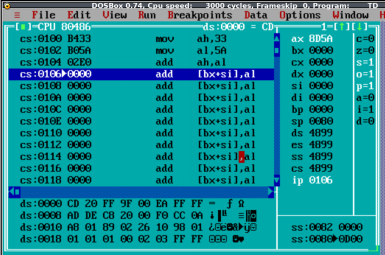
\includegraphics[width=0.7\linewidth]{res/homework_1/fig1.png}
				\caption{执行第一组语句后的状态}
				\label{fig:stat1}
			\end{figure}
			\begin{figure}[H]
				\centering
				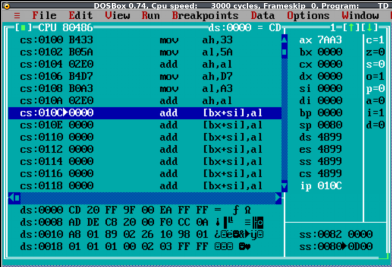
\includegraphics[width=0.7\linewidth]{res/homework_1/fig2.png}
				\caption{执行第二组语句后的状态}
				\label{fig:stat2}
			\end{figure}
			\begin{figure}[H]
				\centering
				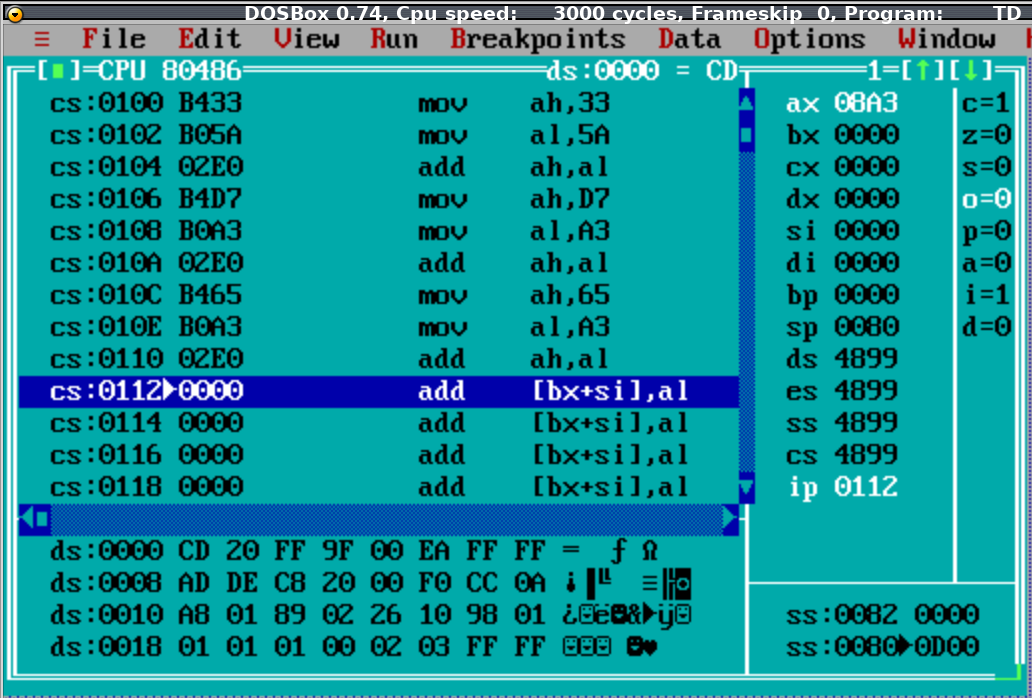
\includegraphics[width=0.7\linewidth]{res/homework_1/fig3.png}
				\caption{执行第三组语句后的状态}
				\label{fig:stat3}
			\end{figure}
		\item 输入3.1.1中剩下的两组指令,分别执行后所得结果如\ref{fig:stat4}和\ref{fig:stat5}所示,可以看看出,在求差运算中,如果两组书均视为有符号数,且A>B,则SF=0, OF=0, CF=1运算产生了进位,若两组数均视为无符号数,且A>B,则SF=0, OF=0, CF=0。未产生借位。这说明无论是有符号数还是无符数,在内存中一律看做是无符号数来处理。
			\begin{figure}[H]
				\centering
				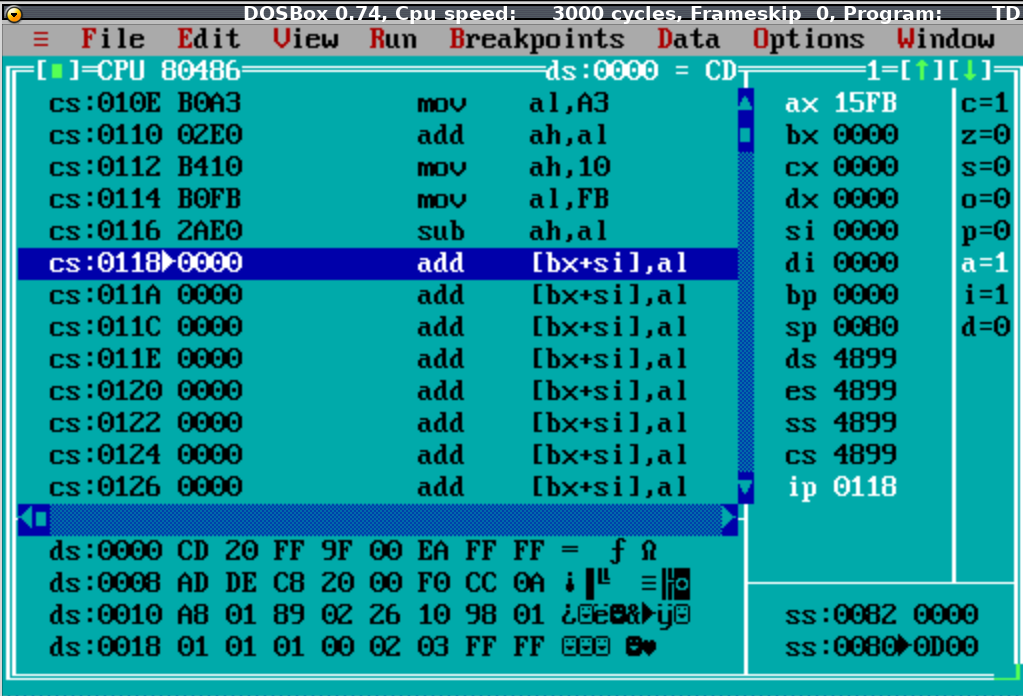
\includegraphics[width=0.7\linewidth]{res/homework_1/fig4.png}
				\caption{执行10H-(-5H) 后的状态}
				\label{fig:stat4}
			\end{figure}
			\begin{figure}[H]
				\centering
				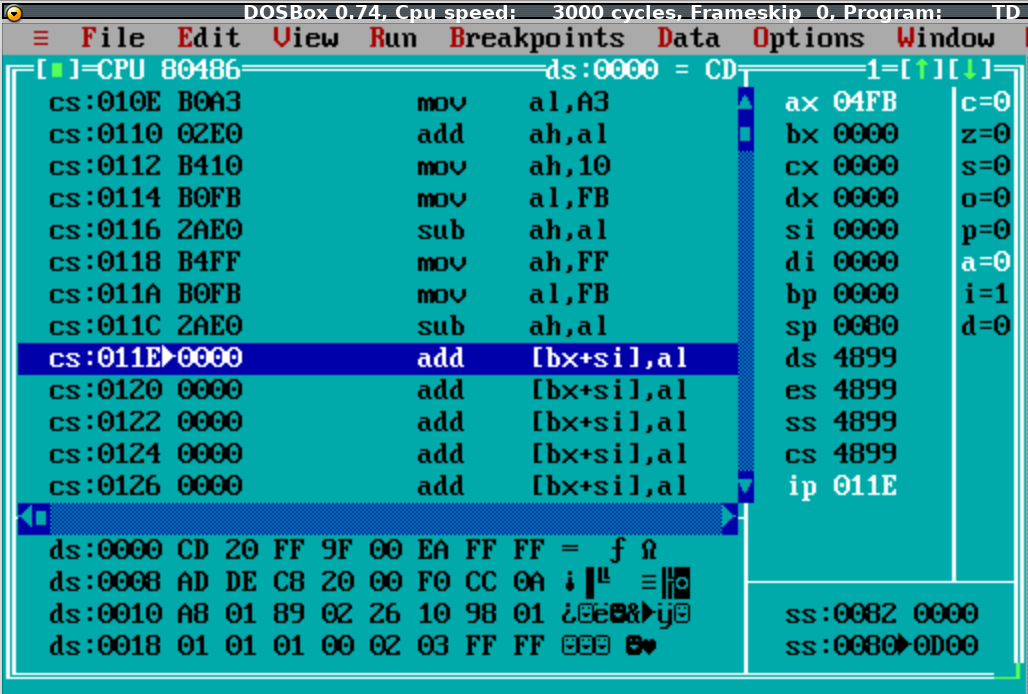
\includegraphics[width=0.7\linewidth]{res/homework_1/fig5.png}
				\caption{执行FFH-(-5H) 后的状态}
				\label{fig:stat5}
			\end{figure}
	\end{enumerate}

	\subsection{任务二}
	\subsubsection{设计思想及存储单元分配}

	求一个数的立方值可以用乘法运算实现,也可以造一立方表,运行时查表实现。依据本次实验的要求,此处用查表法。输入数据为0至9中任一自然数(可以考虑判断输入值的范围是否合乎要求),用一字节单元存放其值;输出数据是该数的立方,用一字单元存放其值。\par

	存储单元分配 \par
	\begin{itemize}
		\item X:字节变量X中存放键入的自然数x。
		\item XXX:字变量XXX中存放x的立方值。
		\item TAB:立方表的首地址。表中共10项,每项占一个字,依次存放0-9的立方值。从表的结构可知,x的立方值在表中的存放地址与x有如下的对应关系:
		\item (TAB + 2 * x) = x的立方值
		\item 对于每个键入的x,从字单元TAB + 2 * x之中取出的数据便是其立方值。
		\item 从键盘接受数字使用1号系统功能调用,此时送入AL之中的是x的ASCII码而不是x的真值。所以,要首先将x的ASCII码换成x的真值,然后用TAB + 2 * x计算x的立方值的存放地址,按此地址查到x的立方值。
		\item INPUT:字节存储区,用于存放提示信息。
	\end{itemize} \par

	寄存器分配 \par
	\begin{itemize}
		\item EBX:存放x的真值,利用带比例因子的变址寻址方式访问立方表。
		\item AX、DX:临时寄存器。
	\end{itemize}

	\subsubsection{流程图}
	\begin{center}
	\begin{tikzpicture}[node distance=2cm]
		\node (start) [startstop] {开始};
		\node (remind) [process, below of=start] {提示用户从键盘输入一个数字};
		\node (input) [process, below of=remind, text width=5cm] {用1号系统功能调用从键盘接收一数字x的ASCII码};
		\node (altox) [process, below of=input] {x的真值\textrightarrow AL\textrightarrow X};
		\node (altox2) [process, below of=altox] {x的真值\textrightarrow EBX};
		\node (move) [process, below of=altox2] {(TAB + [2 $\times$ EBX])\textrightarrow XXX};
		\node (end) [startstop, below of=move] {结束};
		\draw [arrow] (start) -- (remind);
		\draw [arrow] (remind) -- (input);
		\draw [arrow] (input) -- (altox);
		\draw [arrow] (altox) -- (altox2);
		\draw [arrow] (altox2) -- (move);
		\draw [arrow] (move) -- (end);
	\end{tikzpicture}
	\end{center}

	\subsubsection{源程序}
	\begin{codeFont}
		\begin{lstlisting}[gobble=12]
			\.386
			STACK		SEGMENT USE16 STACK
					DB			200 DUP(0)
			STACK		ENDS

			DATA		SEGMENT USE16
			INPUT		DB \'PLEASE INPUT X(0-9):$'
					TAB			DW 0,1,8,27,64,125,216,343,512,729
					X			DB 0
					XXX			DW 0
			DATA		ENDS

			CODE		SEGMENT USE16
			ASSUME		CS:CODE, DS:DATA, SS:STACK
			BEGIN:
					MOV		AX, DATA
					MOV		DS, AX
					MOV		DX, OFFSET INPUT
					MOV		AH, 9
					INT		21H				;显示PLEASE INPUT X(0-9):
					MOV		AH, 1
					INT		21H				;从键盘接受一数字x的ASCII码
					AND		AL, 0FH
					MOV		X, AL			;x的真值 → AL → X
					MOV		EBX,EAX			;x的真值 → EBX
					MOV		AX, TAB[EBX*2]	; (TAB + [2 * EBX])→ AX
					MOV		XXX, AX			; 保存立方值
					MOV		AH, 4CH
					INT		21H
			CODE		ENDS
			END			BEGIN
		\end{lstlisting}
	\end{codeFont}

	\subsubsection{实验步骤}
	\begin{enumerate}
		\item 准备上机实验环境。
		\item 使用vim录入源程序,存盘文件名为CUBE.ASM。使用MASM 6.0汇编源文件。即MASM CUBE;观察提示信息,若出错,则用编辑程序修改错误,存盘后重新汇编,直至不再报错为止。
		\item 使用连接程序LINK.EXE将汇编生成的CUBE.OBJ文件连接成执行文件。即LINK CUBE;若连接时报错,则依照错误信息修改源程序。之后重新汇编和连接,直至不再报错并生成CUBE.EXE文件。
		\item 执行该程序。即在命令行提示符后输入CUBE后回车,观察执行现象。准备输入数字3进行测试,观察执行的结果。
		\item 使用TD.EXE观察CUBE的执行情况。即 TD  CUBE.EXE <CR>
			\begin{enumerate}
				\item 观察CS、IP、SP、DS、ES、SS的值。
				\item 单步执行开始2条指令,观察DATA的实际值,以及DS的改变情况。
				\item 观察SS:0至SS:SP区域的数据值。
				\item 观察DS:0开始数据区,找到各变量在数据段中的位置和值。
				\item 观察第三条语句中源操作数的值,是否和INPUT变量的偏移地址相同。
				\item 执行第3至7条指令,输入数字3。观察AL的值是否为33H。
				\item 执行到MOV  AX, TAB[EBX*2],观察源操作数的具体值。
				\item 执行MOV  XXX, AX,观察目的操作数的形式。到数据段中观察XXX的值是否是3的立方值。
				\item 依次输入0~9,观察结果是否都正确。
				\item 输入字母A,逗号标点等,观察运算结果。
			\end{enumerate}
		\item 将程序重新装入TD中(或将CS:IP重置到MOV AH,9的位置),在执行9号功能调用之前,用TD将数据段中INPUT缓冲区的‘\$’(24H)改成其他数值(如00H),再执行9号功能调用,观察现象。
		\item 当调用1号功能时,若输入大写字母‘A’,则送到XXX的值是哪个存储单元的值;若输入的是‘K’,则送到XXX的值又是哪个存储单元的值。
	\end{enumerate}

	\subsubsection{实验记录与分析}
	\begin{enumerate}
		\item 实验环境条件:i7 3.6GHz,8G内存;Archlinux下DOSBox0.74;VIM.EXE 7.3;MASM.EXE  6.11; LINK.EXE 5.2; TD.EXE 3.1。\\
			汇编源程序时,汇编程序没有出现错误。\\
			连接过程显示了一个警告:LINK: warning L4201: no stack segment。\\
			这指示了程序没有堆栈段,但对程序的正常测试不产生影响,因为程序中灭有用到堆栈段,故忽略之。

		\item 执行之后在新的一行上显示了字符串PLEASE INPUT X(0-9):(如\ref{fig:rundirect}所示)
			\begin{figure}[H]
				\centering
				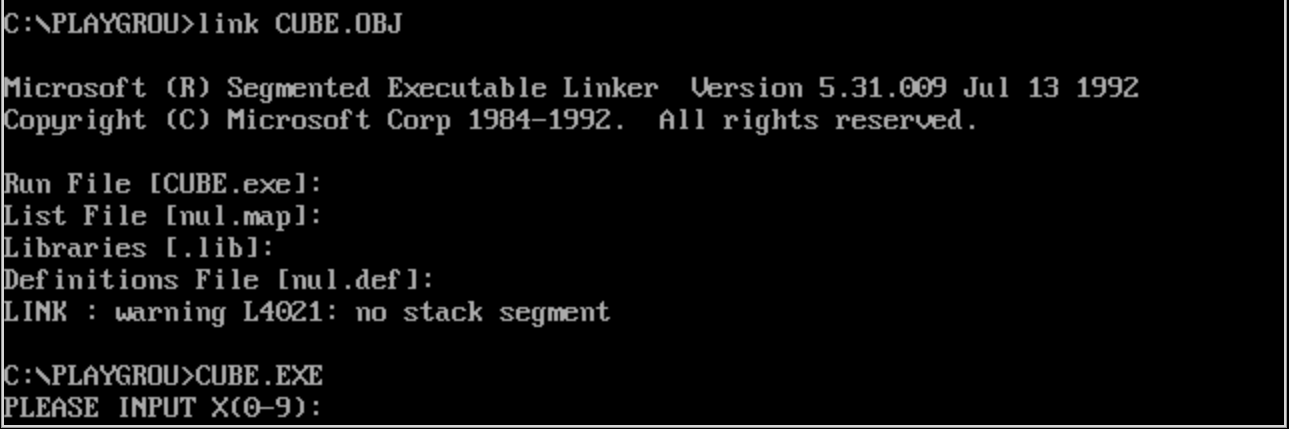
\includegraphics[width=0.8\linewidth]{res/homework_1/fig6.png}
				\caption{直接执行程序}
				\label{fig:rundirect}
			\end{figure}
			输入3之后在冒号后显示了一个3,程序就退出到命令行提示符。说明程序执行基本正常,但由于结果没有显示,所以需要用TD去观察计算结果是否正确。

		\item 用TD调入CUBE.EXE后
			\begin{enumerate}
				\item (CS)=0000H、(IP)=0000H、(SP)=0000H、(DS)=0884H、(ES)=0884H、(SS)=0893H。可从段首址取值的不同得知代码段、数据段、堆栈段处在不同位置,且前后次序是数据段、堆栈段、代码段。
				\item 单步执行开始2条指令,DATA的值=08A1H,(DS)→0884H。观察到TD的数据显示区被切换到了ES:0,若还希望显示DS:0,就需要用Goto指令重新设定。发现此时数据段才是程序的实际位置,各个段的实际次序为堆栈段、数据段、代码段,这与源程序定义各段的次序一致。
				\item SS:0至SS:SP区域的数据值在程序没有执行时均为0。单步执行一次后靠近栈顶的几个字发生了变化,不知为何?
				\item DS:0开始数据区存放了INPUT变量为首址定义的字符串。EA=15H开始存放TAB立方值表。EA=29H存放X(当前值为0);EA=30H存放XXX(当前值为0)。
				\item TD中显示的第三条语句为MOV DX,0000,源操作数的值和INPUT变量的偏移地址相同(均为0)。
				\item 输入数字3。AL的值从24H变成了33H。
				\item MOV  AX, TAB[EBX*2]在TD显示的形式为MOV AX,[2*EBX+00000015]说明TAB代表的EA=00000015H,且是按照双字处理的。
				\item MOV  XXX, AX在TD显示的形式为MOV [002A],AX。执行后DS:(002A)=001BH(即27)是3的立方。(如图\ref{fig:dsvalue}所示)。
					\begin{figure}[H]
						\centering
						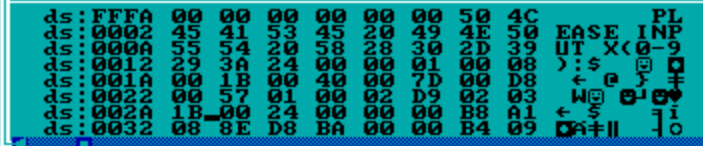
\includegraphics[width=0.8\linewidth]{res/homework_1/fig7.png}
						\caption{DS:(002A)的值}
						\label{fig:dsvalue}
					\end{figure}
				\item 为了方便起见,打开Watchs窗口,输入X和XXX,直接观察X和X的3次方的运行结果,并分别输入0-9,发现X的立方值计算均正确。X=9时的运算结果如下\ref{fig:xisnine}所示
					\begin{figure}[H]
						\centering
						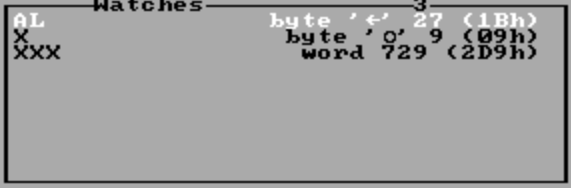
\includegraphics[width=0.8\linewidth]{res/homework_1/fig8.png}
						\caption{当X为9时的结果}
						\label{fig:xisnine}
					\end{figure}
				\item 当输入的是字母A时,在进行AND AL, 0FH 的时候讲‘A’的ASCII码截断为了1,因此计算出来的立方值为1,当输入的是逗号的时候,在进行AND AL, 0FH的时候将AL截断为了12,超出了X的预计范围,ebx为0CH, 取到了TAB[2*12]的界外值,在实际操作中为0。
			\end{enumerate}

		\item 重新载入程序,进行9好系统调用前,将INPUT字符串末尾的’\$’改为‘0‘,然后继续进行系统调用,输出结果如\ref{fig:errorout}所示。可以看出,由于没有遇到终结字符,系统中断一直输出知道遇到了’\$’字符。因此在仅有的程序编写中要尤其注意不要忘记终结字符,否则会导致输出错误。
			\begin{figure}[H]
				\centering
				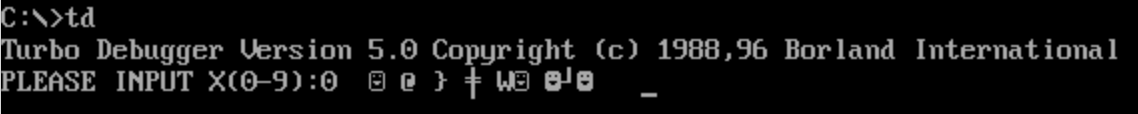
\includegraphics[width=0.8\linewidth]{res/homework_1/fig9.png}
				\caption{错误的输出结果}
				\label{fig:errorout}
			\end{figure}

		\item 重新加载程序,若输入的是‘A’,在与0FH进行‘与’操作后变为了1,因此XXX的值是TAB[1]的值,若输入的是‘K’,在进行与操作后AL的值为0BH,所以TAB[2×EBX]为TAB[22]实际读取的是XXX的高位字节和XXX的后一个字节组成的双字,实际结果也验证了这一想法(见\ref{fig:inputk})
			\begin{figure}[H]
				\centering
				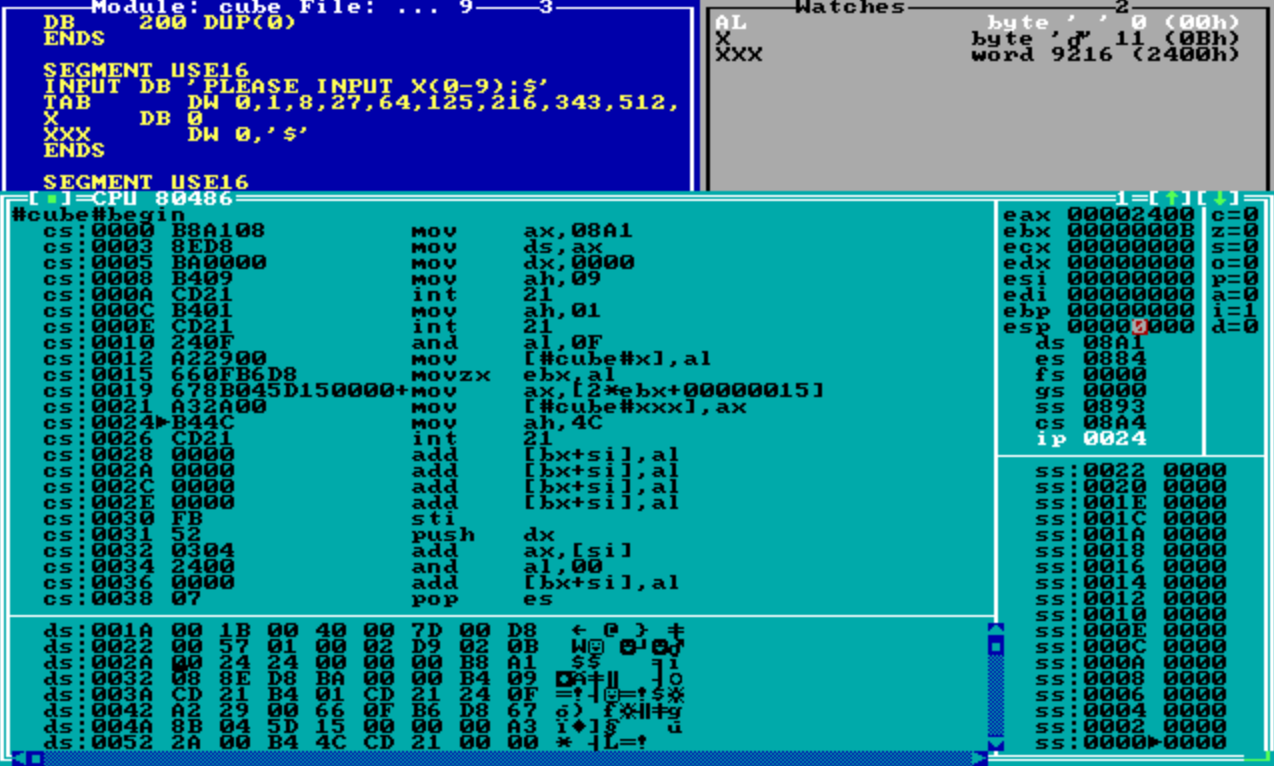
\includegraphics[width=0.8\linewidth]{res/homework_1/fig10.png}
				\caption{输入‘K’的运行结果}
				\label{fig:inputk}
			\end{figure}
	\end{enumerate}

	\subsection{任务三}
	\subsubsection{设计思想}
	原程序的功能是在LOPA的十次循环中,将BUF1的值一一对应复制到BUF2中,将BUF1中的每个值加上1然后一一对应复制到BUF3中,将BUF1中的值加上4然后一一对应复制到BUF4中。\par
	目的是将原程序改为使用变址实现同样的功能。原程序使用是寄存器寻址,要将其改为变址寻址,可以将BX作为计数器,同时作为变址寻址使用的寄存器

	\subsubsection{存储单元分配}
	BUF1到BUF4存储位置不变,依然在DATA区,计数器由CX变为BX,同时BX作为变址寻址寄存器,这样就省去了寄存器寻址所需的寄存器。

	\subsubsection{流程图}
	\begin{center}
		\begin{tikzpicture}[node distance=1.5cm, scale=0.6]
			\node (start)[process]{开始};
			\node (init)[process, below of=start]{初始化DS段};
			\node (init2)[process, below of=init]{初始化BX为0};
			\node (store)[process, below of=init2]{将BUF[1]暂存到AX中};
			\node (axtobuf2)[process, below of=store]{AX\textrightarrow BUF2[BX]};
			\node (incax)[process, below of=axtobuf2]{AX++};
			\node (axtobuf3)[process, below of=incax]{AX\textrightarrow BUF3[BX]};
			\node (incax2)[process, below of=axtobuf3]{AX+=3};
			\node (axtobuf4)[process, below of=incax2]{AX\textrightarrow BUF4[BX]};
			\node (incbx)[process, below of=axtobuf4]{BX++};
			\node (judge)[decision, below of=incbx, aspect=2.5]{BX==10?};
			\node (end)[startstop, below of=judge]{结束};
			\draw [arrow] (start) -- (init);
			\draw [arrow] (init) -- (init2);
			\draw [arrow] (init2) -- (store);
			\draw [arrow] (store) -- (axtobuf2);
			\draw [arrow] (axtobuf2) -- (incax);
			\draw [arrow] (incax) -- (axtobuf3);
			\draw [arrow] (axtobuf3) -- (incax2);
			\draw [arrow] (incax2) -- (axtobuf4);
			\draw [arrow] (axtobuf4) -- (incbx);
			\draw [arrow] (incbx) -- (judge);
			\draw [arrow] (judge) -- node[anchor=west]{Y} (end);
			\draw [arrow] (judge.east) -- node[anchor=south]{N} ++(3.0cm, 0) |- (store);
		\end{tikzpicture}
\end{center}

	\subsubsection{源程序}
	以下是修改过后的源程序:\par

	\begin{codeFont}
	\begin{lstlisting}[gobble=8]
		.386

		STACK SEGMENT USE16 STACK
				DB 200 DUP(0)
		STACK ENDS

		DATA SEGMENT USE16
				BUF1 DB 0, 1, 2, 3, 4, 5, 6, 7, 8, 9
				BUF2 DB 10 DUP(0)
				BUF3 DB 10 DUP(0)
				BUF4 DB 10 DUP(0)
		DATA ENDS

		CODE SEGMENT USE16
		ASSUME CS:CODE, DS:DATA, SS:STACK
		START:
				MOV		EAX, BYTE PTR DATA
				MOV		DS, WORD PTR EAX

				MOV		EBX, 0
		LOPA:
				MOV		AL, BUF1[EBX]
				MOV		BUF2[EBX], AL

				INC		AL
				MOV		BUF3[EBX], AL

				ADD		AL, 3
				MOV		BUF4[EBX], AL

				INC		EBX
				CMP		EBX, 10
				JNZ		LOPA
				MOV		AH, 4CH
				INT		21H
		CODE ENDS
		END START
	\end{lstlisting}
	\end{codeFont}

	\subsubsection{实验步骤}
	\begin{enumerate}
		\item 打开dosbox,使用vim录入源程序,保存为24\_MODI.ASM。
		\item 进行修改,将源程序改为3.3.4所示状态。
		\item 使用TASM进行编译,同时生成符号表
		\item 使用TLINK进行链接,生成24\_MODI.EXE,同时链接符号表
		\item 打开TD,装载24\_MODI.EXE
		\item 在watch窗口中添加BUF1、BUF2、BUF3、BUF4、AX、BX
		\item 将ds监视窗口置u于BUF1处
		\item 单步执行,观察AX、BX、BUF1~4的变化情况。
	\end{enumerate}

	\subsubsection{实验记录与分析}
	\begin{enumerate}
		\item 实验环境条件:i7 3.6GHz,8G内存;Archlinux下DOSBox0.74;VIM.EXE 7.3;编译、链接、调试使用TASM套件。编译、链接时没有出现错误。
		\item 直接运行二进制文件,没有任何输出,程序正常推出,说明要进入调试器进一步调试。
		\item 打开TD,装载24\_MODI.EXE。
		\item 在WATCH窗口中添加BUF1~4,BX,AX
		\item 在CMP处添加一断点。初始化完成后界面如图\ref{fig:loadcomplete}所示
			\begin{figure}[H]
				\centering
				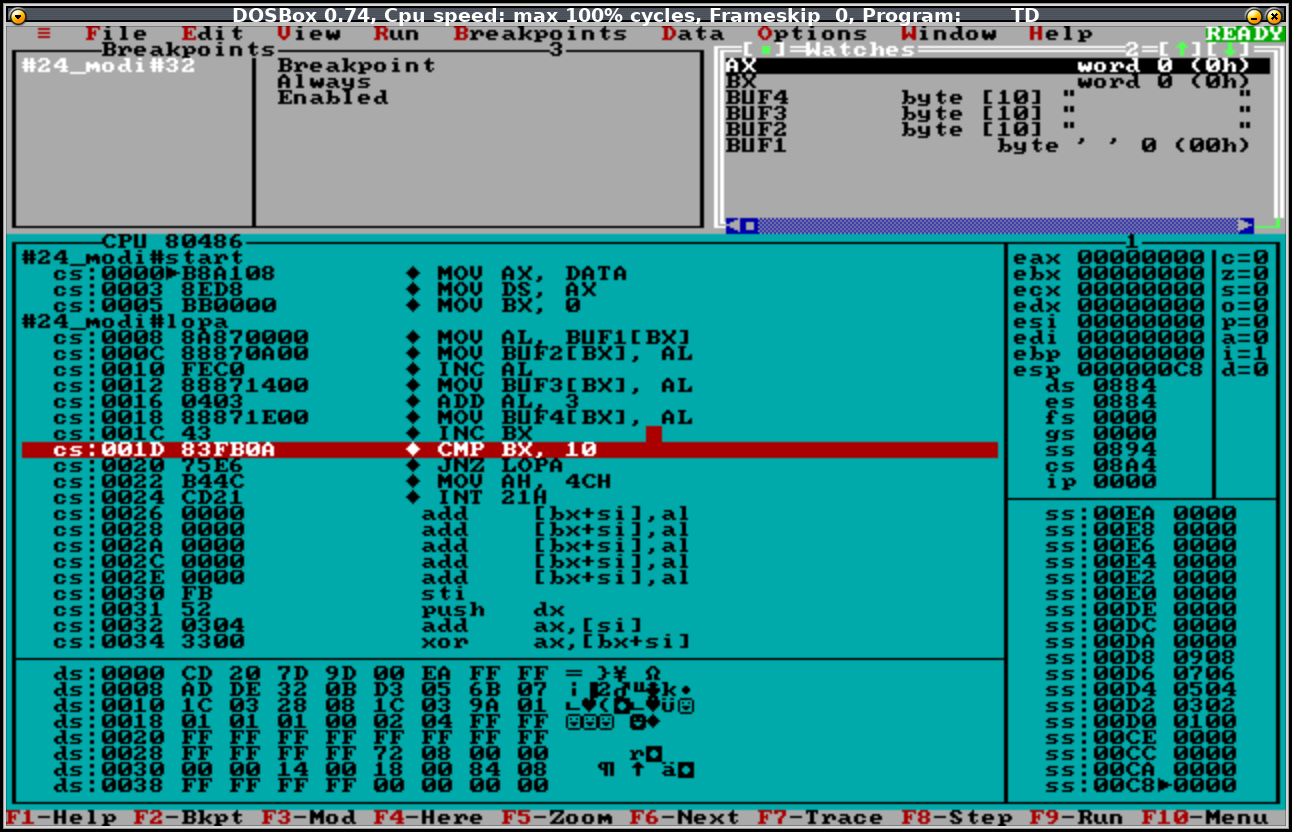
\includegraphics[width=0.8\linewidth]{res/homework_1/fig11.png}
				\caption{程序装载完成界面}
				\label{fig:loadcomplete}
			\end{figure}
		\item 单步执行,观察寄存器和内存的变化,发现在执行到断点处时,寄存器和内存的变化均如意料进行,第一次执行到断电处时内存如图\ref{fig:firstbreakpoint}所示,其中光标所在处为BUF1地址。
			\begin{figure}[H]
				\centering
				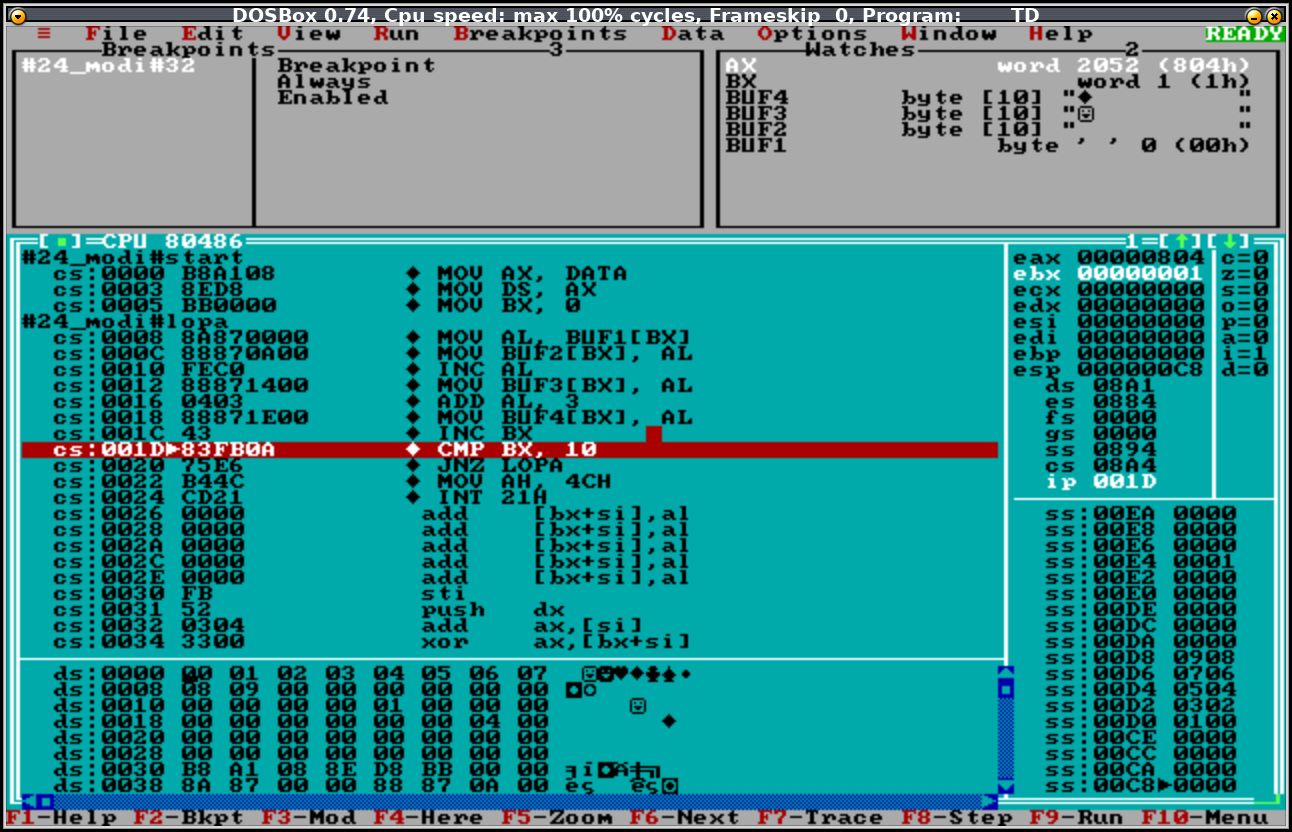
\includegraphics[width=0.8\linewidth]{res/homework_1/fig12.png}
				\caption{第一次运行到断点}
				\label{fig:firstbreakpoint}
			\end{figure}
		\item 然后使用run指令(F9)观察到每一次循环均将BUF1中对应的值移动到了BUF2、BUF3、BUF4中(BUF3中加上了1、BUF4中加上了3)
		\item 一直运行到第十次(最后一次)运行到断点,结果如图\ref{fig:loopcomplete}所示,BUF1中所有的数均已正确转移。
			\begin{figure}[H]
				\centering
				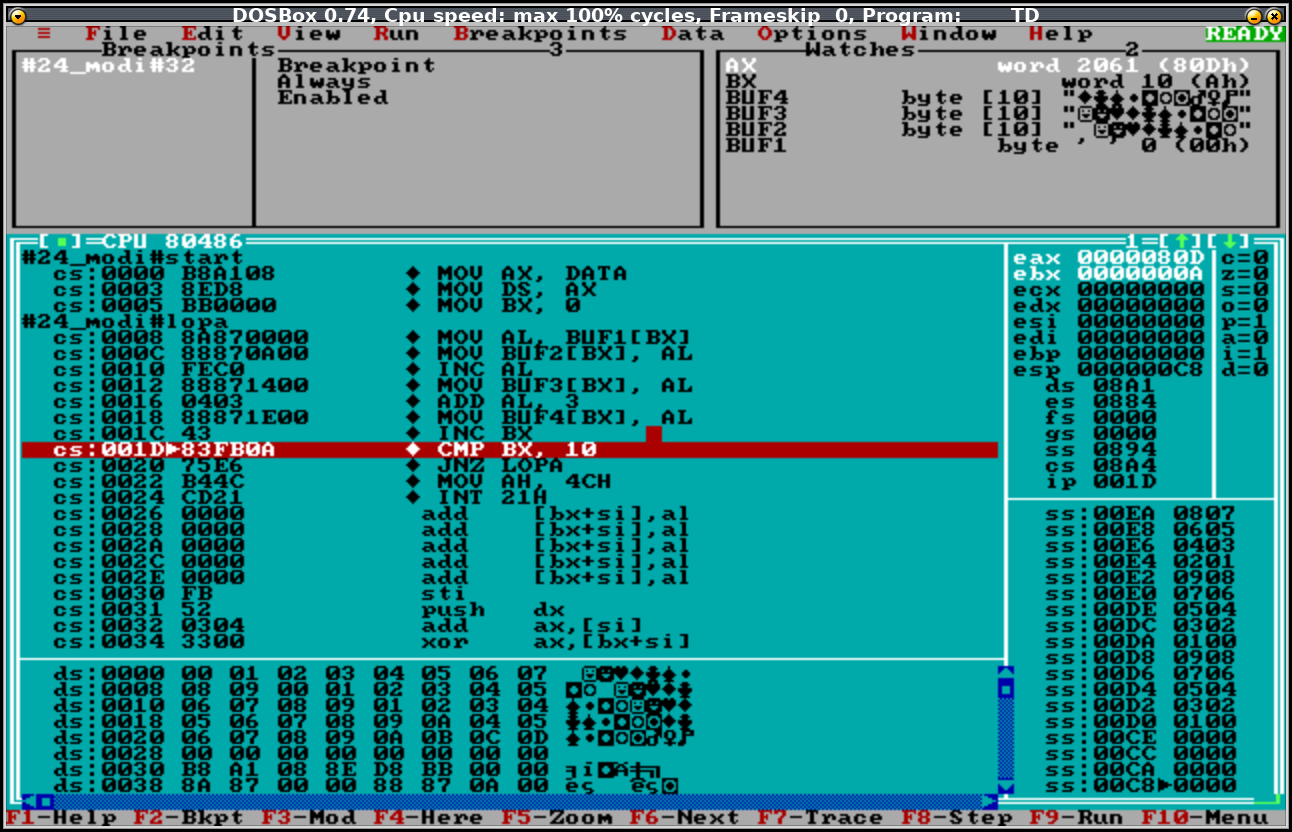
\includegraphics[width=0.8\linewidth]{res/homework_1/fig13.png}
				\caption{最后一次循环完成}
				\label{fig:loopcomplete}
			\end{figure}
	\end{enumerate}

	\subsection{任务四}

	\subsubsection{设计思想}
	本程序要求实现一个学生成绩查询程序,并对输入的信息,查找到的学生的成绩做处理后存储并且输出。为了清晰结构,将程序分为以下几个部分:输入部分,查找部分(比较部分),成绩计算部分和输出部分,详细设计如下:
	\begin{itemize}
		\item 总体上,所有的字符串输出使用int 21H的09H号中断,需要输出的内容全部保存在数据段;所有需要输出的字符使用int 21H的02H号中断,需要输出的字符使用立即数表示;需要输入数据则使用int 21H的0AH号中断,需要输入的数据存在数据区的数据缓冲区中。由于本题所需输入的数据仅为学生的姓名,且长度不超过10,因此数输入据缓冲区的长度为10;
		\item 输入部分,对用户输入的数据进行判断,若为回车字符(DH),则判定为非法输入,提示重新输入;若为’q\r’(71H, 0DH),则判断为退出,直接终止程序;若为一串字母(含空格符,即ascii码为20H, 41H~5AH, 61H~7AH)时,判断为姓名,进入查找部分继续执行;其余所有情况判断为非法输入,要求重新输入。
		\item 查找部分,对于预先存在数据区的姓名进行遍历,在遍历的主循环中:对姓名的每一个字进行逐字匹配,一旦发现失配则匹配不成功,进入下一个循环;若同时匹配到结尾,表明匹配成功,跳转进入计算部分;若所有的姓名均遍历完成仍没有匹配成功者,则表明姓名不存在,重新进入输入部分。
		\item 计算部分,利用MUL,DIV指令对查找到的姓名所对应的三个成绩进行计算,所得的结果存入对应姓名的平均成绩存储区中,然后对所得成绩进行评级,以90, 80, 70, 60为分界,落入五个区间的成绩分别评级为A, B, C, D, F并进行显示输出。
	\end{itemize}

	\subsubsection{存储单元分配}
		大部分数据存储于数据段中,其中包括:
		\begin{enumerate}
			\item 100个随机生成的姓名数据,和分数,每一项占14字节,其中姓名占个字节,不足的部分用0补齐,语文、数学、英语成绩分别占用一个字节,平均成绩占用一个字节。
			\item 输入缓冲区,一共13个字节,第一个字节存缓冲区长度,第二个字节存缓冲区读入字节数,第3到地13个字节存放读入的字符。
			\item 提示用户输入姓名的字符串。
			\item 提示用户姓名输入错误的字符串。
			\item 显示学生信息的提示字符串。
		\end{enumerate}

	\subsubsection{流程图}
		图\ref{fig:flowchart2}展示了程序的主要流程
		\begin{figure}[h]
			\centering
			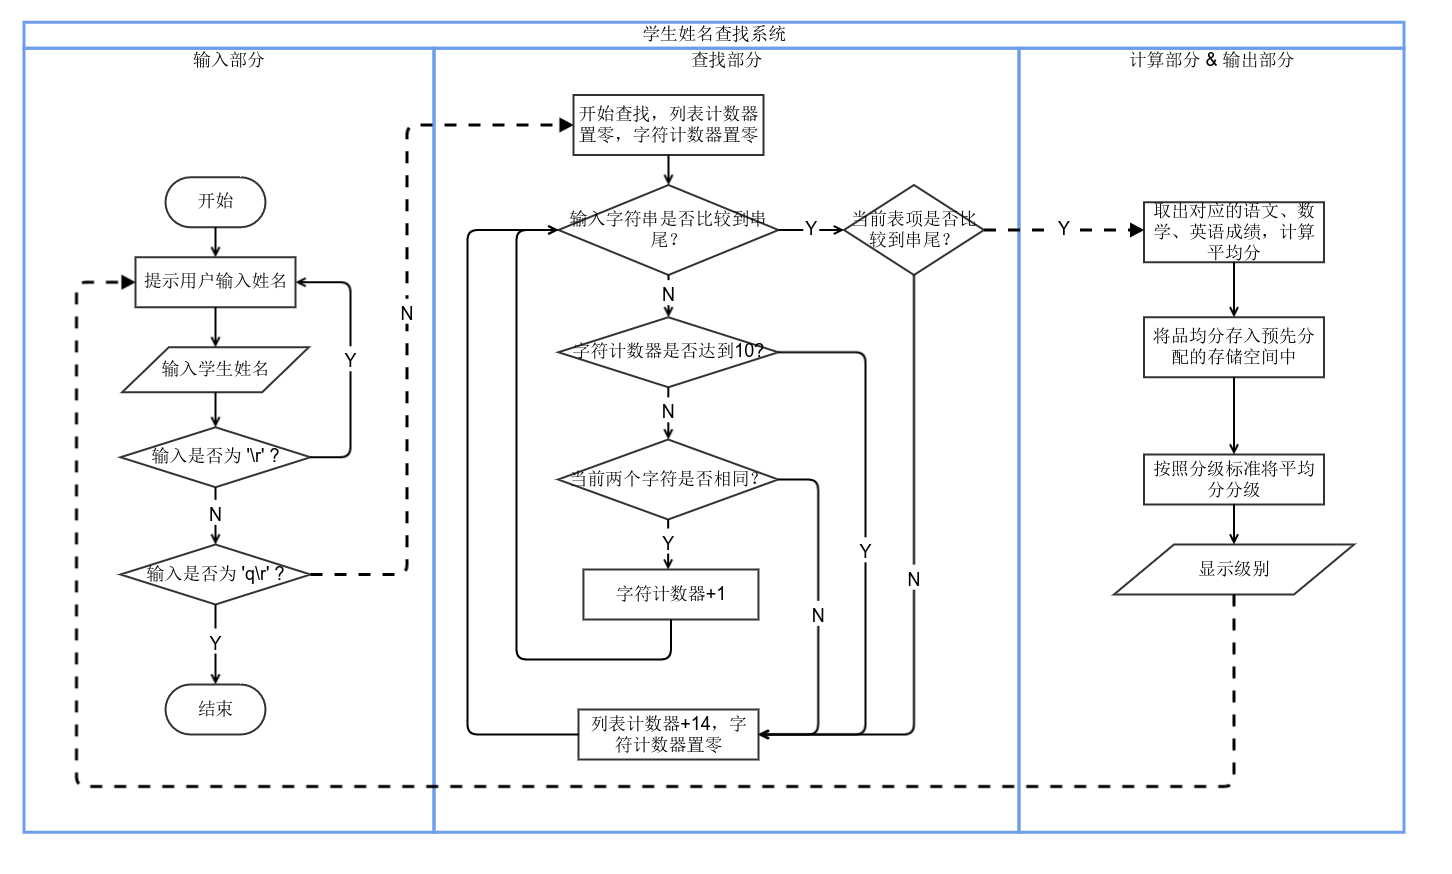
\includegraphics[width=1.0\linewidth]{res/homework_1/fig14.png}
			\caption{程序总体流程}
			\label{fig:flowchart2}
		\end{figure}

	\subsubsection{源程序}
	源程序详见附录部分。(第\pageref{code:1_4}页)

	\subsubsection{实验步骤}
		对应本程序的测试分为以下几个步步骤:
		\begin{enumerate}
			\item 编译链接,修正编译器和连接器所提示的错误。
			\item 直接运行,观察程序对输入的处理和输出有无明显错误。
			\item 进入Turbo Debugger调试,分别对输入部分,查找部分,计算部分和输出部分进行测试,观察各个部分的功能是否正常。
			\item 对于输入部分,分别测试存在于表中的姓名,不存在于表中的姓名,以及非法字符,观察程序是否能够正常处理。
			\item 对于查找部分,更改查找部分的数据集,使得查找部分能够覆盖每一个跳转分支,并观察两个计数器的变化情况,判断程序是否正常执行。
			\item 对于计算部分,手动修改计算部分的三门科目的成绩,观察计算所得的结果是否正确,以及是否有溢出产生。
		\end{enumerate}

	\subsubsection{实验记录分析}
		\begin{enumerate}
			\item 实验环境条件:i7 3.6GHz,8G内存;Archlinux下DOSBox0.74; VIM.EXE 7.3; TASM 5.0、TLINK 5.0、TD 5.0编译、链接、调试套件。\\
				汇编和链接过程均没有出现错误。
			\item 编译完成,直接执行STUDENT.EXE,出现提示字符串’Please input the name of the student:’
			\item 输入一个列表中已经存在的姓名,如Sixu Hu<\r> 程序显示该学生平均分所对应的等级,并继续提示用户输入学生姓名。
			\item 输入一个列表中不存在的姓名,如asdf<\r>,程序提示该学生不存在,并要求重新输入。
			\item 直接输入回车,程序再次要求输入学生姓名。
			\item 输入q<\r>,程序直接退出。2~6步输出结果如图\ref{fig:fig15}所示,初步表明程序能够正常运行。
				\begin{figure}[h]
					\centering
					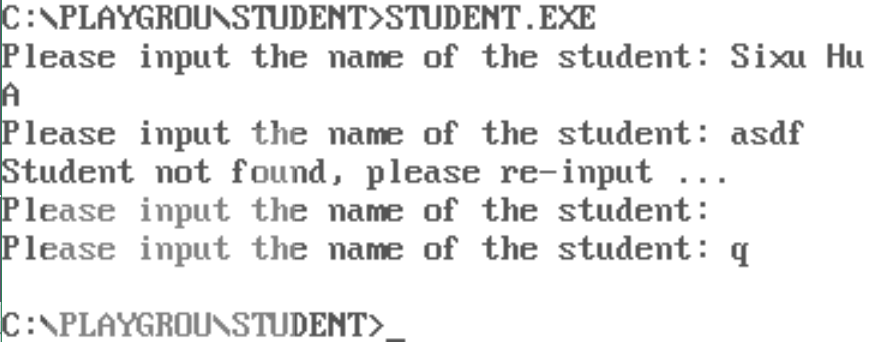
\includegraphics[width=0.8\linewidth]{res/homework_1/fig15.png}
					\caption{直接运行程序的输出结果}
					\label{fig:fig15}
				\end{figure}

			\item 在平均分的计算部分以及存储部分需要进入调试器观察内存的具体情况。
			\item 打开TD,加载STUDENT.EXE,在输入部分、查找部分和计算部分的入口分别插入断点,然后执行,监视列表计数器esi、字符计数器ecx,列表当前字符tab[esi+ecx],输入串当前字符in\_buff[ecx],按下F9-Run运行并观察变化。
			\item 测试输入功能:在提示输入姓名后,输入Sixu Hu<\r>,程序运行到查找入口断点处,在内存窗口跳转到in\_buff输入缓冲区首地址处,观察内存,发现输入缓冲区存储的内容正确,由于dos会自动限制输入字符个数,因此输入不会超过10个字符。内存窗口如图\ref{fig:fig16}所示。这表明输入功能正常。
				\begin{figure}[h]
					\centering
					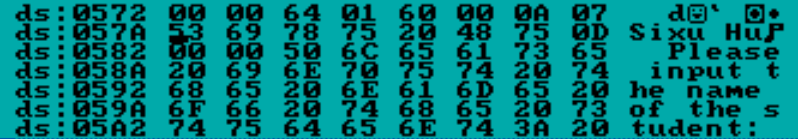
\includegraphics[width=0.8\linewidth]{res/homework_1/fig16.png}
					\caption{输入姓名后的内存缓冲区}
					\label{fig:fig16}
				\end{figure}

			\item 测试查找功能:单步执行,在每一个判断跳转处观察当前的列表计数器以及字符计数器是否正常,并观察跳转位置是否正常。发现程序在首次遇到不匹配字符时即刻进入列表下一列,与预想一致。而当两个字符串同时匹配到结尾时,程序跳转到计算部分。
			\item 重复执行程序,改变输入名字,确保覆盖到查找部分的条件判断的每一种情况和每一个跳转分支,每层循环的次数测试尽可能覆盖到0, 1, 2, m, n-1, n, n+1次,其中n为最大可能循环次数(对外层而言为99,在存在对应名字的情况下)且2<m<n,以确保查找部分运作无误,所用到的测试用名字如表\ref{tab:nametable}所示(分支对照表见图\ref{fig:fig17})。经过测试,没有错误出现,查找部分功能正常。
				\begin{table}[H]
					\centering
					\caption{测试用姓名及覆盖分支}
					\label{tab:nametable}
					\begin{tabular}{c l l c}
						\hline\hline
						姓名& 分支& 内层循环次数覆盖& 外层循环次数 \\
						\hline
						Ju Song & 1,2,3,6,8 & 7 & 0 \\
						Jin Lu & 1,2,3,6,7,8 &1,6 & 1 \\
						Yin Ma & 1,2,3,6,7,8 & 0,6 & 2 \\
						Sixu Hu & 1,2,3,6,7,8 & 0,7 & 4 \\
						Dong Ma & 1,2,3,6,7,8 & -- & 98 \\
						Jia	Bai & 1,2,3,6,7,8 &	-- & 99 \\
						Asdf & 1,2,3,6,7,8 & -- & 100 \\
						JuAAA & 1,2,3,6,7,8 & 2 & 100 \\
						A & 1,2,3,4,6,7,8 & 0 & 100 \\
						\hline
					\end{tabular}
				\end{table}
				\begin{figure}[h]
					\centering
					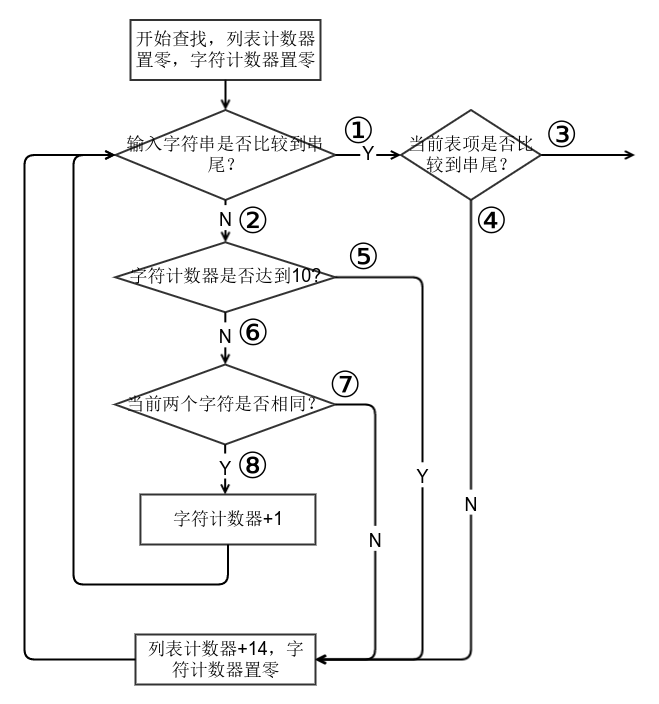
\includegraphics[width=0.6\linewidth]{res/homework_1/fig17.png}
					\caption{分支对照图}
					\label{fig:fig17}
				\end{figure}

			\item 测试计算部分:程序跳转到测试部分的入口处,手工修改内存中的程序数据,分别测试平均成绩为0分时,平均成绩为满分时以及可能造成溢出时的成绩数据,然后单步执行程序,观察平均分的计算以及存储是否正常运行,级别判断是否正确以及程序是否溢出。
			\item 测试表明,即使总分数全部取最大,即100,100,100,在执行加权以后总分为350,没有超过一个16位寄存器的表示范围,而乘法的积与除法的被除数均为16位寄存器,因此不会溢出。
			\item 至此,所有主要功能测试完成,没有发现异常。输出部分由于程序较为简单,在调试其他部分的同事观察每次输出无误,即表明输出部分功能正常。
		\end{enumerate}

		\newpage
		\section{总结与体会}

		通过任务1的实验,让我知道了TD不仅可以调入现成的执行程序进行调试,而且能随时输入和测试单一一条指令是否正确,执行效果如何,这将方便未来的学习过程。另外,通过观察,计算机内的加减运算,无论是否有符号数,对应的标志位都是设定好了的,如何使用这些标志,完全由程序员选择的指令来决定,这就要求我们编写程序时要理解好题目的语义,选择合适的指令语句,而不是我写了个负数交给汇编程序,系统就会自动选择有符号指令的。 \par
		任务2的实验表明,源程序定义的段的次序,与调到内存中段的次序是有对应关系的。但数据段开始没有被赋值到实际的数据段首址中,需要执行了我们的相关赋值语句后才变得实际有效。另外,各种寻址方式在内存中确实不如源程序直观了,但可以看到变量的偏移值都被很好的计算出来了,我们可以通过源程序中变量与内存中对应位置的信息获得该变量的偏移地址,方便我们在数据显示区输入该地址,查看对应的变量内容。\par
		任务2中若输入0~9之外的字符,结果其实是没有意义的。要解决这个问题,可以增加对输入的值的范围进行判断的语句,超出范围时报错,并要求重新输入。\par
		在任务4中,我充分的学习到了使用汇编编写一个完整的程序、并且不断调试直到它能够正常运行的方法,题目4综合了前面三道题所学的几乎所有知识,并且让我们创造自己的程序,极大地增强了我们的编码能力和对代码的解读能力。同时,由于大量的调试工作的进行,我更加熟悉了Turbo Debugger 的各种便于调试的功能和调试的方法(如打断点,监视,查找,跳转,录制宏等),提高了我的综合能力。\par
		本次上机不仅提高了编程水平,熟悉了工具的使用,而且加深了对一些知识的理解。主要的经验教训如下: \par
		首先,更加感受到实验前准备的意义。例如:上机前准备越充分(如先编好源程序,制定好准备做的一些步骤),上机的时候目的越明确,可以解决较多的问题。\par
		其次,录入程序时要注意一些细节,比如中文分号、字母O等问题,虽然汇编程序指出其所在行有错,但很难发现具体是哪个符号错了,耽误了不少时间。TD在程序细节的观察、动态修改方面有很大的作用,要主动用TD的调试功能帮助自己发现、理解与解决问题。\par
		最后,由于操作不够熟练,时间比较紧张等原因,还有些问题需要以后进一步解决,如堆栈中数据变化的原因、各个段在内存中存放的关系、是否可跟踪到INT 21H中去、多次调入程序时初始的段值是否相同等等。\par


%% Part Two %%%%%%%%%%%%%
%%%%%%%%%%%%%%%%%%%%%%%%%
\newpage
\part{程序执行时间与代码长度优化}
	\section{实验目的与要求}
	\begin{enumerate}
		\item 熟悉汇编语言指令的特点,掌握代码优化的基本方法;
		\item 理解高级语言程序与汇编语言程序之间的对应关系。
	\end{enumerate}

	\section{实验内容}
	\subsection[任务1]{任务1: 观察多重循环对CPU计算能力消耗的影响}
	{\textbf{要求}}: \par
	若有m个用户在同一台电脑上排队使用实验一任务四的程序,想要查询成绩列表中最后一个学生``wangwu的''平均成绩,那就相当于将实验一任务四的程序执行了m次。为了观察从第一个用户开始进入查询至第m个用户查到结果之间到底延迟了多少时间,我们让实验一任务四的功能二和功能三的代码重复执行m次,通过计算这m次循环执行前和执行后的时间差,来感受其影响。由于功能一和功能四需要输入、输出,速度本来就较慢,所以,没有纳入到这m次循环体内(但可以保留不变)。请按照上述设想修改实验一任务四的程序,并将m值尽量取大(建议$ m \geqslant 1000 $,具体数值依据实验效果来改变,逐步增加到比较明显的程度,比如秒级延迟),以得到较明显的效果。\par
	{\textbf{提示}}: \par
	\begin{enumerate}
		\item 在进入功能二之前增加m次循环的初始化工作,在功能三结束之后增加m次循环的条件判断和转移语句。
		\item 学校汇编教学网站的软件下载中提供了显示当前时间“秒和百分秒”的子程序。若在m次循环前调用一下该子程序,m次循环执行完之后再调用一下该子程序,就能在屏幕上观察并感受到执行循环前后的时间差(时间差值需要自行手工计算,当然,你也可以选用网站上另一个计时程序,它是可以帮你计算好差值的)。注意,由于虚拟机环境下CPU会被分时调度,故该时间差值会因计算机运行环境与状态的不同而不同。
	\end{enumerate}

	\subsection[任务2]{任务2:对任务1中的汇编源程序进行优化}
	{\textbf{要求}}: \par
	优化工作包括代码长度的优化和执行效率的优化,本次优化的重点是执行效率的优化。请通过优化m次循环体内的程序,使程序的执行时间尽可能减少10\%以上。减少的越多,评价越高。 \par
	{\textbf{优化方法提示}}: \par
	首先是通过选择执行速度较快的指令来提高性能,比如,把乘除指令转换成移位指令、加法指令等;其次,内循环体中每减少一条指令,就相当于减少了m*n条指令的执行时间,需要仔细斟酌;第三,尽量采用32位寄存器寻址,能有更多的机会提高指令执行效率。

	\subsection[任务3]{任务3:观察用C语言实现的实验一任务四中功能一的程序与汇编语言实现的程序的差异}
	{\textbf{要求}}: \par
	用汇编语言和C语言分别实现实验一任务四中功能一的功能(对汇编语言而言,就是把实验一中相关程序摘取出来成为独立的程序),对比两种语言实现的程序的代码情况,观察和总结C语言编写程序和自己的汇编语言程序的对应关系及差异,总结其中可以简化的地方。 \par
	{\textbf{提示}}: \par
	采用反汇编方法观察C语言编写生成的执行程序时,首先观察程序的整体结构特点(包括段的情况),然后重点分析、比较输出输入字符串对应的代码。

	\newpage
	\section{实验过程}
	\subsection{任务一}
	\subsubsection{设计思想}
	将查找最后一个学生的成绩并计算平均分的步骤进行重复,重复多次以达到时间统计的误差不超过3\%,并且可以忽略循环控制部分所消耗的时间。最后直接通过时间显示函数观察所消耗的时间,从而观察查找部分和计算部分对于CPU消耗的影响。同时,可以考虑单独测试循环部分和计算部分循环同样次数所消耗的时间,从而统计两个部分分占用的时间比例。
	\subsubsection{流程图}
	\begin{tikzpicture}[node distance=2cm]
		\node (start) [virtualstartstop] { 开始(原) };
		\node (main1) [process, below of=start] { 输入部分 };
		\node (main2) [process, below of=main1] { 查找部分 };
		\node (main3) [process, below of=main2] { 计算以及输出部分 };
		\node (end) [virtualstartstop, below of=main3] { 结束(原) };

		\node (sidestart) [startstop, right of=start, node distance=7cm] {开始(计时)};
		\node (outtime1) [process, right of = main1, node distance=4cm] {显示当前时间};
		\node (outtime2) [process, right of = main3, node distance=4cm] {显示当前时间};
		\node (sideend) [startstop, right of=end, node distance=7cm] {结束(计时)};

		\node (deltatime) [right of=main2, node distance=4cm]{间隔时间};

		\draw [arrow, dashed] (start) -- (main1);
		\draw [arrow] (main1) -- (main2);
		\draw [arrow] (main2) -- (main3);
		\draw [arrow, dashed] (main3) -- (end);

		\draw [arrow] (sidestart) |- (outtime1);
		\draw [arrow] (outtime1) -- (main1);
		\draw [arrow] (main3) -- (outtime2);
		\draw [arrow] (outtime2) -| (sideend);

		\draw [arrow, dotted] (deltatime) -- (outtime1);
		\draw [arrow, dotted] (deltatime) -- (outtime2);
	\end{tikzpicture}

	\subsubsection{源程序变更}
	源程序变更详见附录部分。(第\pageref{code:2_1}页)

	\subsubsection{实验步骤}
	修改后的程序的测试分为以下几个步骤:
	\begin{enumerate}
		\item 修改源程序,进行编译链接,根据编译链接的错误修改程序并重复编译链接,直到没有错误出现。
		\item 直接运行,输入最后一个学生的名字,观察有无运行时错误出现,若有,根据错误修改程序,并重新编译,链接,运行。
		\item 重复运行,在相同条件下统计运行时间间隔并求平均值。
		\item 修改源程序中时间测试循环的位置,同条件下重复运行,测试每个部分所占时间比例,并统计平均值。
	\end{enumerate}

	\subsubsection{实验记录与分析}
	\begin{enumerate}
		\item 实验环境条件:i7 3.6GHz,8G内存;Archlinux下DOSBox0.74; VIM.EXE 7.3; TASM 5.0、TLINK 5.0、TD 5.0编译、链接、调试套件。 {\textbf{模拟CPU频率3000cycle/sec}}
		\item 修改源程序,使查找及输出部分重复30000次,并在循环前后打印当前时间。
		\item 编译时出现了一个错误:标号超出距离范围。观察程序,由于时间测试循环的标号距离跳转位置太远,因此不能进行断转移,于是对程序作出以下修改:
			\begin{itemize}
				\item 将标号`loop\_big\_s:'更改为`loop\_big\_s label far'
				\item 将跳转语句`loop loop\_big\_s' 更改为`dec cx;	jmp far ptr loop\_big\_s'
			\end{itemize}
			修改后编译链接成功
		\item 直接执行程序,输入最后一个学生的名字。发现由于循环了30000变输出,刷新了屏幕,而DOS的显示缓冲区不能向上滚动,从而不能显示开始时间,因此修改源代码,将计算部分的显示输出释掉,并重新编译运行。
		\item 此时软件能够显示开始的时间和结束的时间。然而由于时间显示子程序的局限性,只能显示秒和百分秒,不能显示分钟,因此当运行跨过一分钟的末尾或者超过一分钟的时候,读数将不能正常显示。
		\item 重新修改时间显示子程序,令其能够显示分钟,多次运行程序。
		\item 并调节时间测量循环的位置,分别测量查找部分和计算部分所占用的时间比例,从而缩小程序热点所在的位置。计算所得结果如表\ref{tab:table1}所示,查找+计算部分的程序输出如图\ref{fig:time}所示,另外两部分的时间测试输出结果格式与之相同。
			\begin{table}[H]
				\centering
				\caption{30000次循环的时间测量结果}
				\label{tab:table1}
				\begin{tabular}{c c c c}
					\toprule
					{\bfseries 次数} & {\bfseries 查找+计算部分/秒} & {\bfseries 查找部分/秒} & {\bfseries 计算部分/秒} \\
					\cmidrule(lr){1-1}\cmidrule(lr){2-4}
					1 & 20.99 & 20.92 & 0.72 \\
					2 & 20.92 & 20.92 & 0.65 \\
					3 & 20.93 & 20.93 & 0.71 \\
					4 & 20.93 & 20.94 & 0.66 \\
					5 & 20.98 & 20.96 & 0.66 \\
					\cmidrule(lr){1-1}\cmidrule(lr){2-4}
					平均 & 20.95 & 20.934 & 0.68 \\
					\bottomrule
				\end{tabular}
				\begin{figure}[H]
					\centering
					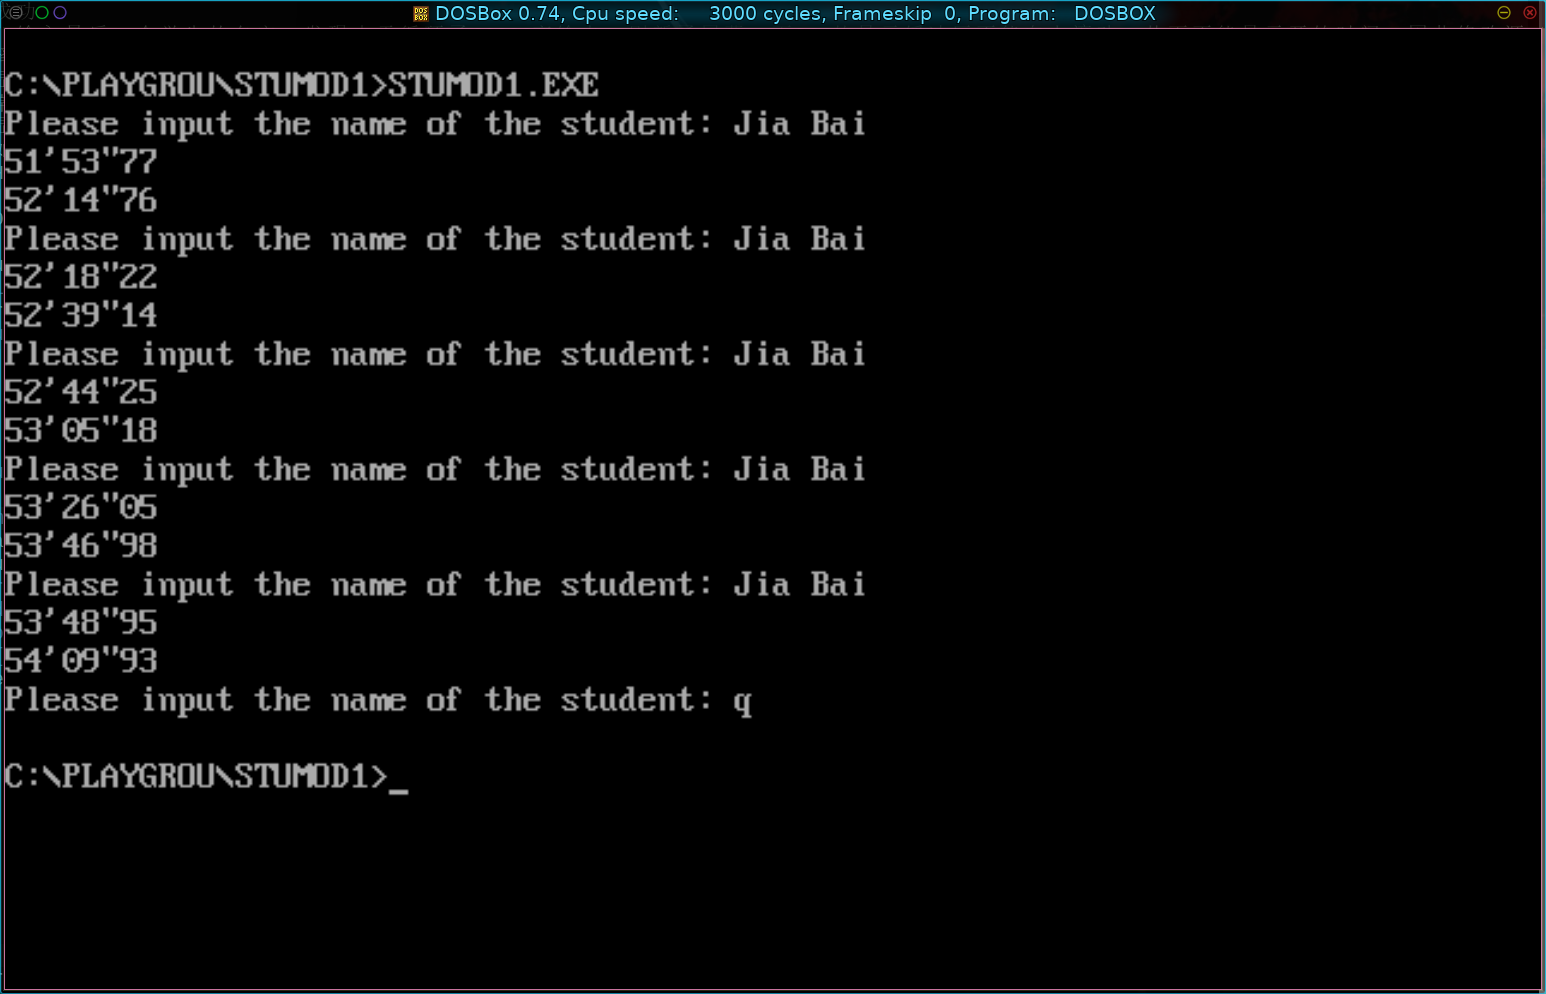
\includegraphics[width=0.9\linewidth]{res/homework_2/time.png}
					\caption{时间测试 查找+计算部分 运行输出}
					\label{fig:time}
				\end{figure}
			\end{table}
			通过结果可以看出,相较于计算部分,查找部分占据了主要的时间,因此在优化的时候主要需要对查找部分进行优化而不是计算部分。
	\end{enumerate}

	\subsection{任务二}
	\subsubsection{优化思想}
	\begin{itemize}
		\item 在任务1的基础上对源程序进行优化,保留查找部分+计算部分的计时循环。
		\item 由于程序的主体逻辑在编写的过程中已经对查找时间进行了优化,在遇到不匹配时会直接进入下一循环,故不更改主体逻辑。
		\item 由于相对于计算部分而言,查找部分占据99\%以上的时间(见表\ref{tab:table1}),故主要对查找部分进行优化。
		\item 在查找主循环中,为了程序编写方便,使用了esi和edi两个计数器。现优化性能,只使用其中一个计数器进行计数。
		\item 在查找部分的字符比较次级循环中,由于添加了不必要的判断(即输入字符串到达串尾`\textbackslash r'字符时判断表内字符串是否到达第10个字符且不为0),而实际上由于输入字符串被限制在9个字符(除掉`\textbackslash r'字符),因而不可能出现这种情况,故将此判断删去。
		\item 由于dos系统限制,输入字符串的最后一个字符一定是'\r',故不需要判断是否已经比较到第10个字符以避免数组越界。将这一部分删除。
	\end{itemize}

	\subsubsection{流程图变更}
	\begin{tikzpicture}[node distance=3cm]
		\node (beg) [process, text width=5cm] {开始查找,列表计数器置零,字符计数器置零};
		\node (ask1) [decision, below of=beg] {输入字符串是否比较到串尾?};
		\node (ask2) [decision, dashed, below of=ask1] {字符计数器是否达到10?};
		\node (ask3) [decision, below of=ask2] {当前两个字符是否相同?};
		\node (ask4) [decision, right of=ask1, node distance=8cm] {当前表项是否比较到串尾?};
		\node (add1) [process, below of=ask3] {字符计数器+1};
		\node (end) [process, below of=add1, node distance=4cm,text width=4cm] {列表计数器+14,字符计数器置零};

		\draw [arrow]			(beg) -- (ask1);
		\draw [arrow, dashed]	(ask1) -- node [very near start, anchor=west]{N} (ask2);
		\draw [arrow, dashed]	(ask2) -- node [very near start, anchor=west]{N} (ask3);
		\draw [arrow, dashed]	(ask2) -- node [very near start, anchor=south]{Y} ++(5.5cm,0) |- (end);
		\draw [arrow]			(ask1.south) .. controls ++(5cm,-1cm) and ++(5cm, 1cm) .. (ask3.north);
		\draw [arrow]			(ask1) -- node [very near start, anchor=south]{Y} (ask4);
		\draw [arrow]			(ask3) -- node [very near start, anchor=west]{Y} (add1);
		\draw [arrow]			(add1) |- ++(0, -2cm) -- ++(-4cm,0) |- (ask1);
		\draw [arrow]			(end) -- ++(-5cm, 0) |- (ask1);
		\draw [arrow]			(ask4) |- node [very near start, anchor=west]{N} (end);
		\draw [arrow]			(ask3) -- node [very near start, anchor=south]{N} ++(4cm,0) |- (end);
	\end{tikzpicture}

	\subsubsection{源程序变更}
	源程序变更详见附录部分。(第\pageref{code:2_2}页)

	\subsubsection{实验步骤}
	\begin{enumerate}
		\item 对任务一的程序进行修改,并编译链接,若有错误,重复修改、编译、链接步骤,直到没有错误出现为止。
		\item 直接运行程序,输入最后一个学生的名字,观察有无运行时错误,若有,重复修改、编译、链接、运行的步骤,直到没有错误出现为止。
		\item 在和任务一相同的条件下(即模拟CPU频率相同,输入相同)重复运行程序,统计运行时间结果。
		\item 将得到的时间结果与任务一所得结果进行对比,观察优化程度。
	\end{enumerate}

	\subsubsection{实验记录与分析}
	\begin{enumerate}
		\item 实验环境条件:i7 3.6GHz,8G内存;Archlinux下DOSBox0.74; VIM.EXE 7.3; TASM 5.0、TLINK 5.0、TD 5.0编译、链接、调试套件。 {\textbf{模拟CPU频率3000cycle/sec}}
		\item 按照优化思想对源程序进行修改,主要是去除不需要的判断和跳转,优化查找时间。
		\item 对修改后的源程序进行编译、链接。在编译、链接的过程中没有出现错误。
		\item 在与任务一相同的条件下直接运行程序,输入最后一个学生的名字,没有出现运行时错误。
		\item 重复运行优化后的程序,记录并统计平均值,统计结果如表\ref{tab:table2},程序输出如图\ref{fig:time3}。
			\begin{table}[H]
				\centering
				\caption{优化前后查找+输出时间对比}
				\label{tab:table2}
				\begin{tabular}{ c c c c c }
					\toprule
					次数 & 优化前/秒 & 优化后/秒 & 节约时间/秒 & 优化程度/\%  \\
					\cmidrule(lr){1-1}\cmidrule(lr){2-5}
					1 & 20.99 & 16.92 & 4.07 & 19.39 \\
					2 & 20.92 & 16.98 & 3.94 & 18.83 \\
					3 & 20.93 & 16.92 & 4.01 & 19.16 \\
					4 & 20.93 & 16.97 & 3.96 & 18.87 \\
					5 & 20.98 & 16.92 & 4.06 & 19.35 \\
					\cmidrule(lr){1-1}\cmidrule(lr){2-5}
					平均 & 20.95 & 16.94 & 4.01 & 19.12 \\
					\bottomrule
				\end{tabular}
			\end{table}
			\begin{figure}[H]
				\centering
				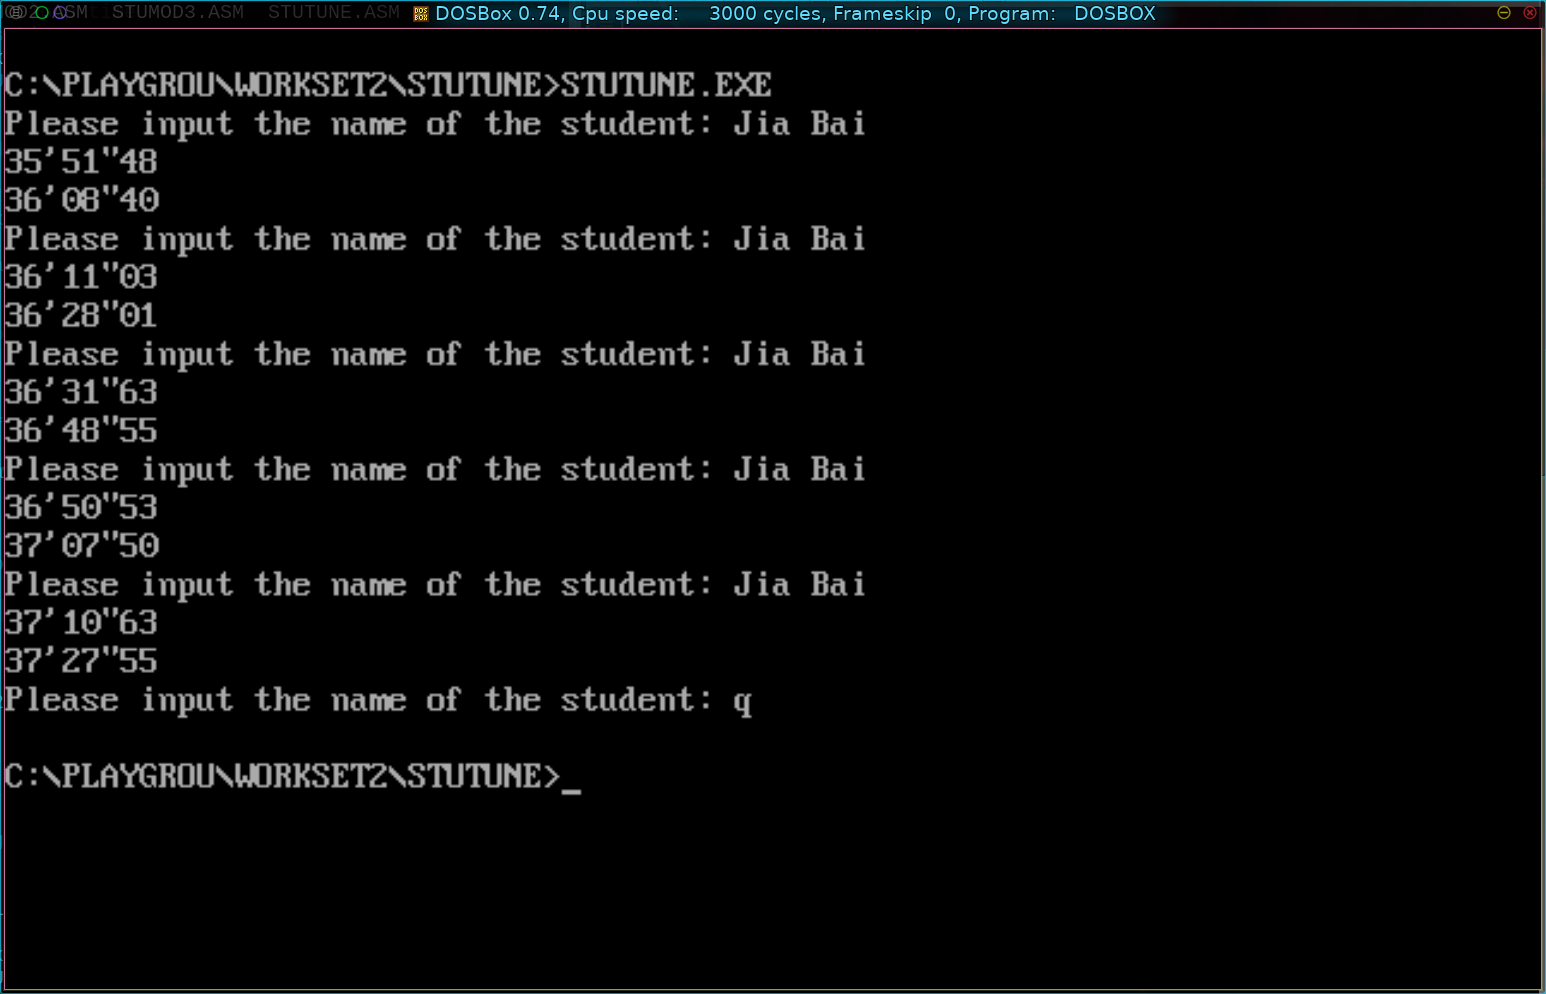
\includegraphics[width=0.9\linewidth]{res/homework_2/time3.png}
				\caption{优化后程序运行输出}
				\label{fig:time3}
			\end{figure}
		\item 可以看出,对于循环较多的部分以及程序的热点有针对性的优化能够大幅度的提高程序的性能。
	\end{enumerate}

	\subsection{任务三}
	\subsubsection{设计思想}
	\begin{itemize}
		\item 使用C语言实现与汇编语言相同的功能,并进行反汇编后和汇编语言进行比对,了解编译器是如何将C语言转换为汇编语言的。
		\item 通过观察反汇编的内容,了解手写汇编与编译器编译相比的优势和劣势。
	\end{itemize}

	\subsubsection{流程图}
	以下是C语言编写功能一程序的流程图: \par
	\begin{center}
		\begin{tikzpicture}[node distance=2cm]
			\node (beg) [startstop] {开始};
			\node (notice) [io, below of=beg] {提示输入姓名};
			\node (get) [io, below of=notice] {输入学生姓名};
			\node (judge1) [decision, below of=get] {输入是否为``\textbackslash r''?};
			\node (judge2) [decision, below of=judge1] {输入是否为``q\textbackslash r''?};
			\node (proc) [process, dashed, below of=judge2] {进行下一阶段运算};
			\node (end) [startstop, below of=proc] {结束};

			\draw [arrow] (beg) -- (notice);
			\draw [arrow] (notice) -- (get);
			\draw [arrow] (get) -- (judge1);
			\draw [arrow] (judge1.west) --  node [anchor=south] {Y} ++(-2cm,0cm) |- (notice);
			\draw [arrow] (judge1) -- node [anchor=west] {N} (judge2);
			\draw [arrow] (judge2.west) --  node [anchor=south] {Y} ++(-2cm,0cm) |- ($(end.north)+(0cm,0.5cm)$) -- (end) ;
			\draw [arrow] (judge2) -- node [anchor=west, near start] {N} (proc);
			\draw [arrow] (proc) -- (end);
		\end{tikzpicture}
	\end{center}

	\subsubsection{源代码}
	源代码详见附录部分。(第\pageref{code:2_3}页)
	\subsubsection{实验步骤}
	\begin{itemize}
		\item 对于汇编而言,将第一部分(输入部分)单独提取进行编译。
		\item 对于C语言而言,实现与输入部分相同的功能,并在相同的环境中进行编译。
		\item 分别运行、调试C程序和汇编程序,以确保功能正常。
		\item 对比C程序转换成的汇编和原汇编程序,了解编译器对于C语言的汇编实现、编译器的实现与手写汇编的区别。
	\end{itemize}

	\subsubsection{实验记录与分析}
	\begin{itemize}
		\item 实验环境条件:i7 3.6GHz,8G内存;Archlinux下DOSBox0.74; VIM.EXE 7.3; TASM 5.0、TLINK 5.0、TD 5.0编译、链接、调试套件。 {\textbf{C语言编译使用Borland Turbo C++ 3.0}}
		\item 按照设计思想编写C程序,使用TCC进行编译,运行程序,程序能够正常运行,运行输出如图\ref{fig:output1}所示。
			\begin{figure}[h]
				\centering
				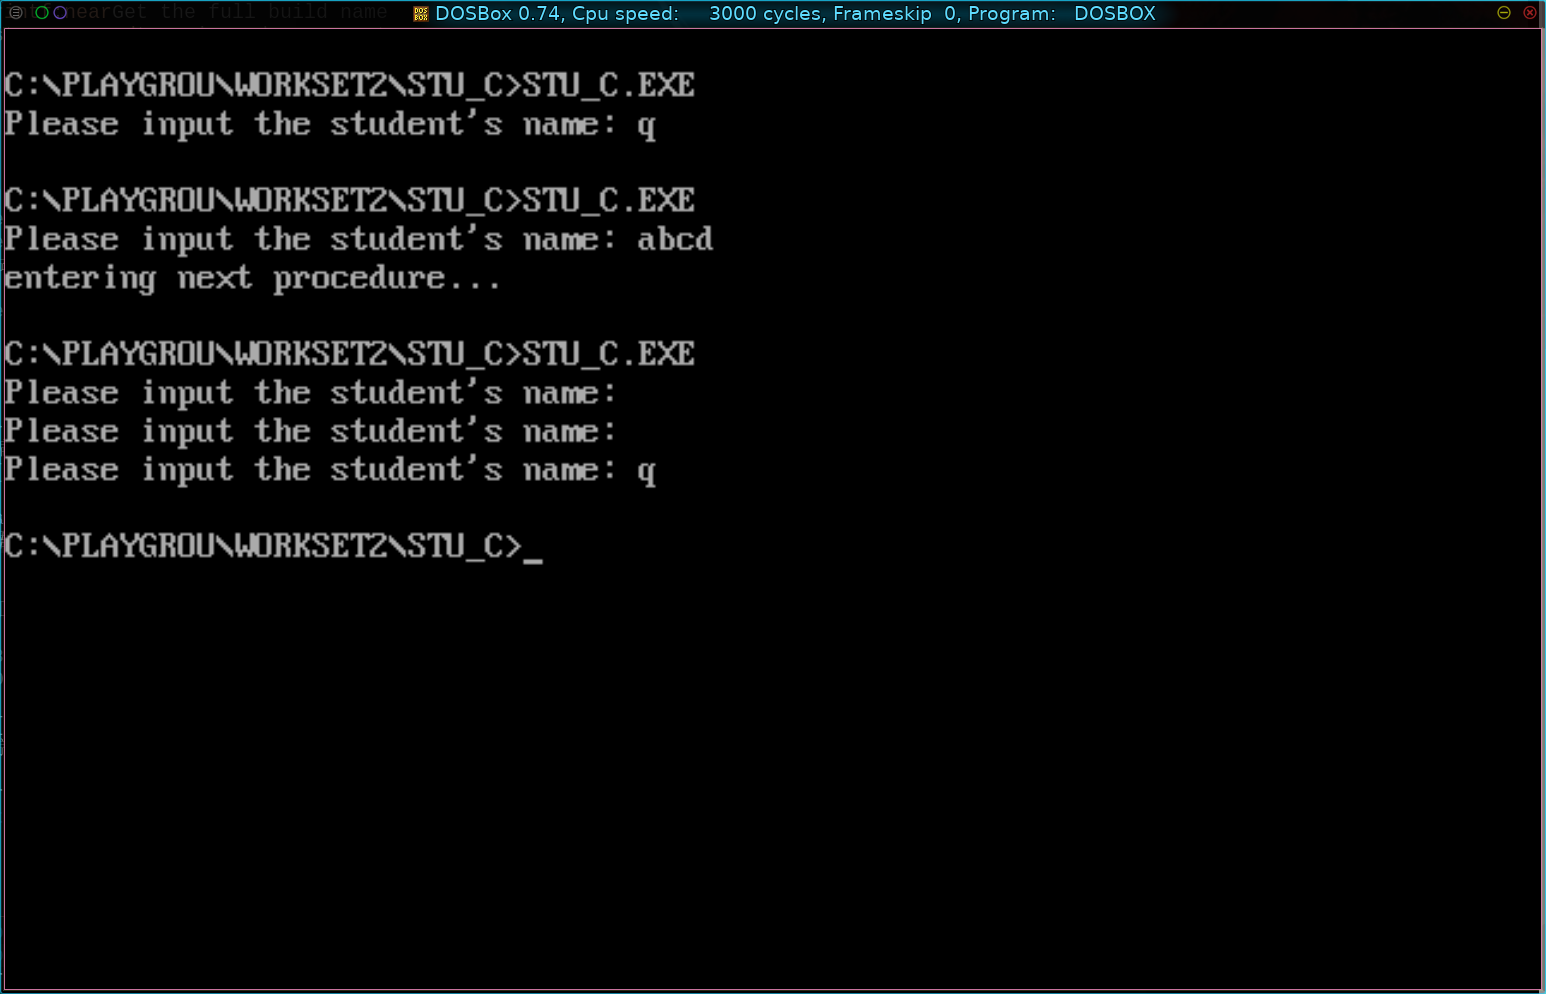
\includegraphics[width=0.9\linewidth]{res/homework_2/output1.png}
				\caption{C语言程序编译运行输出}
				\label{fig:output1}
			\end{figure}
		\item 编译提取出的汇编程序,使用TASM进行编译,运行程序,程序运行结果与实验一任务四功能一的输出相同。
		\item 使用TCC -S <input-file>对C语言进行翻译,得到汇编结果如源代码部分所示。
		\item 将手写的汇编和生成的汇编进行对比,可以发现,在长度上,生成的汇编长度远大于手写的汇编长度。但对于源程序的编写而言,C语言的编写逻辑更为清晰,代码更为简洁。
		\item 对于生成的汇编代码进行分析,发现在程序主题部分(main函数部分)被定义到\_TEXT段中,所有用到的常量字符串都被预先定义到\_DATA段中,而数组也事先在DATA段中分配了空间。
		\item 在输入输出时,直接调用了printf和scanf子程序,并通过push ax压栈传递参数。
		\item 对于判断和跳转部分,编译器生成的代码和手写的代码非常相似,均为使用cmp进行比较以后根据标志位进行跳转。
		\item 可以看出,C语言和汇编在编写这一程序时,主要不同之处在于输入与输出部分,使用汇编编写时直接使用系统中断实现输入与输出,而C语言则是调用子程序进行输入输出,这也是主要的性能差异所在。
	\end{itemize}

	\newpage
	\section{总结与体会}
	通过任务一的实验,我了解到了测量汇编程序对于CPU占用的基本方法,并成功的对程序进行了基本的分析,定位了占用CPU较多的程序段,为下一步的针对性优化打下了基础。 \par
	在任务二中,动手实践对程序的优化使我对汇编语言的指令集有了更为深入的了解,并了解到了程序优化的基本方法以及程序优化的重要性。在汇编程序中,有一些指令可以用另一些更为简洁、高效率的指令所代替,还有一些经过逻辑判断以后发现不需要的分支,这些都构成了优化的主体部分。更为重要的是,我了解到了有针对性优化的重要性。若在第一步中没有对程序进行分段分析,那么我可能会对计算部分段进行较为深入的优化,然而实际上计算部分所占用的时间比例非常小,优化的价值不高,因此对于查找部分的优化才能够显著提高程序性能。\par
	在任务三中,我了解到了编译器将C语言转换为汇编语言的基本途径,以及对于常量、变量、判断以及转移的处理。编译器对于C语言的处理有很强的模式性,例如在调用子程序时总是通过堆栈传参(内联函数除外),不同循环中的跳转指令除标号以外基本一致等。这也导致了在使用C语言的时候有一些可以使用寄存器以及简单指令来提升速度的地方不能得到优化。
	对于输入输出部分,C语言与汇编有较大的区别。C语言常用的输入输出均是通过调用标准库中的函数实现的。在汇编中,除了通过调用函数以外,还可以直接通过系统中断来实现,这样可以在一定程度上节省时间。 \par
	总体而言,这一次实验使我了解到了程序测试与优化的基本方法,了解到了底层语言与高级语言之间的主要区别以及转换关系,这些知识在今后的学习尤其是对程序的优化过程中将会发挥更大的作用。

%% Part Three %%%%%%%%%%%
%%%%%%%%%%%%%%%%%%%%%%%%%
\newpage
\part{模块化程序设计}
	\section{实验目的与要求}
	\begin{enumerate}
		\item 掌握子程序设计的方法与技巧,熟悉子程序的参数传递方法和调用原理。
		\item 掌握宏指令、模块化程序的设计方法。
		\item 掌握较大规模程序的合作开发与调试方法。
		\item 掌握汇编语言程序与C语言程序混合编程的方法。
		\item 熟悉C编译器的基本优化方法。
		\item 了解C语言编译器的命名方法,主、子程序之间参数传递的机制。
	\end{enumerate}

	\section{实验内容}

	\subsection[任务一]{任务一:宏与子程序设计}
	\noindent 进一步修改与增强实验二的学生成绩查询程序的功能,具体要求如下: \par
	\begin{enumerate}
		\item 程序执行时首先显示一个功能菜单:选择1=录入学生姓名和各科考试成绩,2=计算平均分,3=计算排名,4=输出成绩单,5=程序退出。 \par
			提示:由于学生姓名和成绩是通过程序录入的,因此,定义学生成绩表缓冲区时,初始值都可以置零。为避免录入成绩的时间过程太长,假定学生人数在5人左右,具体人数自行决定。每个学生成绩表中增加一个字用来保存排名。平均分的结果只需保留整数部分。
		\item 2人一组,一人负责包括菜单显示、程序退出在内的主程序,以及菜单中的功能1和2;另一人负责菜单中的功能3和4。各自汇编自己的模块,然后连接生成一个程序。注意,在每个模块的开始,注明编写者的名字以及同组同学的名字。
		\item 录入学生姓名和各科考试成绩时,首先显示录入的是第几个学生的信息,然后分别在提示之后输入姓名和各科成绩(可以借鉴书上十进制转二进制的子程序F10T2)。所有学生信息录入完毕后回到菜单显示的位置。姓名及考试成绩的存放、平均分的计算,按照实验二的要求。
		\item 排名的基本要求是按照平均成绩从高到低计算名次,也可以考虑按照指定课程的成绩排名。相同平均分时排名相同,下一个相邻平均分的排名应该是排名在前的所有人数和的下一个数值。输出成绩单的基本要求是依次显示每个学生的姓名、平均成绩和排名,也可以考虑按照指定课程、指定进制的形式显示(可以借鉴书上二进制转十进制的子程序F2T10)。
		\item 将9号和10号DOS系统功能调用定义成宏指令并调用。
	\end{enumerate}

	\noindent {\textbf{提示:}} \par
	\begin{enumerate}
		\item 在TD中跟踪到子程序内部有几种方法?在TD中观察子程序调用和返回时堆栈的变化。
		\item 注意观察FAR、NEAR类型子程序的RET指令的机器码有何不同?观察FAR类型子程序被调用时堆栈的变化情况。
		\item 通过把一个模块拆成多个模块或反之,体会子程序和模块化程序设计的方法,体会模块调用关系图、子程序功能说明、输入/输出说明在程序设计中的作用。
		\item 观察不同模块的可合并段合并后变量偏移地址的变化情况。观察不同段在内存里的放置次序。体会模块间段的定义及其对应的装配方法。
		\item 在编程中使用不同的子程序参数传递方法来编写子程序。
		\item 观察模块间的参数的传递方法,包括公共符号的定义和外部符号的引用,若符号名不一致或类型不一致会有什么现象发生?
		\item 通过TD观察宏指令在执行程序中的替换和扩展,解释宏和子程序的调用有何不同。
		\item 如何使菜单和成绩单显示得更漂亮一点?
		\item EXTRN说明语句放在.386之前或者之后有什么区别?
		\item EXTRN说明的变量的段与段寄存器的关联关系(ASSUME伪指令所表达的信息)是否能带入到本模块中?如果不能带入,是否可以通过加段前缀的方法来解决?
		\item 如何利用宏功能使汇编语言的程序变得更加直观易读?\par
			例:下面是一个利用宏功能直观化后的完整代码段程序,请写出对应的宏定义,并模仿该方式对自己编写的某段程序进行类似的改写。
		\begin{codeFont}
		\begin{lstlisting}[gobble=12]
			,start
			Initial_ds
			GetStringTo   BUF
			DisplayStringFrom  BUF
			ExitToDOS
			EndProgram  code,start
		\end{lstlisting}
		\end{codeFont}
	\end{enumerate}

	\subsection[任务二]{任务二:在C语言程序中调用汇编语言实现的函数}

	对于任务1的程序进行改造,主控程序、以及输入输出等功能用C语言实现,其他功能用独立的汇编语言子程序的方式实现; 在C语言程序中调用汇编语言子程序。\par
	\noindent {\textbf{要求与提示:}} \par
	\begin{enumerate}
		\item 在不同的C语言开发环境中实现与汇编语言程序的混合编程,其操作方法有可能是不同的。请大家选择自己熟悉的C语言开发环境并查找相关的资料完成本实验。
		\item 在实验报告中,比较详细的给出你的开发环境及其实现方法。
		\item 观察C语言编译器中对各种符号的命名规则(指编译器内部可以识别的命名规则,比如,符号名前面是否加下划线``\_'',等),主、子程序之间参数传递的机制,通过堆栈传递参数后堆栈空间回收的方法。
		\item 对混合编程形成的执行程序,用调试工具观察由C语言形成的程序代码与由汇编语言形成的程序代码之间的相互关系,包括段、偏移的值,汇编指令访问C的变量时是如何翻译的,等。
		\item 请尝试在C语言源程序中不合理地嵌入汇编语言的指令语句,达到破坏C语言程序的正确性的目的。比如,在连续的几条C语言语句中间加入一条修改AX寄存器(或DS等其他寄存器)的汇编指令语句,而AX的内容在此处本不该被修改,这样就可观察到破坏C语言程序正确性的效果(该项实验表明:在C语言程序中,若不考虑上下语句翻译成怎样的机器码而随意嵌入汇编指令语句时,有可能存在出错的风险)。
		\item 观察C编译器的优化策略对代码的影响。
		\item 通过调试混合编程的程序,体会与纯粹汇编语言编写的程序的调试过程的差异。
		\item 通过本次实验,希望大家明白:不同的编程语言是可以协同解决一个问题的,而且可以利用不同语言的特点来更好地解决问题;利用汇编语言的知识,能够更好地理解高级语言的内部处理原理与策略,为编写更好的C语言程序、用好C编译器提供支持。
	\end{enumerate}

	\section{实验过程}

	\subsection{任务一}
	\subsubsection{设计思想}
	本任务需要在实验一的基础上,讲程序的功能增加为录入学生信息、计算平均分、计算排名、输出成绩单,同时,将使用较为频繁的小程序段定义为宏。使用模块和宏有如下的优点:
	\begin{itemize}
		\item 将程序模块化可以使程序的条理和逻辑结构更加清晰。
		\item 模块可以多次调用,在需要重复调用某一模块时,可以减少编写代码的工作量。
		\item 在项目较大时,需要多人合作,而模块化的编程可以使不同的人负责不同的模块,分工明确。
		\item 使用模块化编程易于是整个项目增量式的进行,及时有的模块没有编写完成,也可以先测试已完成的模块,增加开发效率。
		\item 在调试的时候,先从总体框架的层面确定问题所在的模块,可以迅速缩小问题的范围,调试方便。
	\end{itemize}
	在学生成绩查找系统中,录入,计算平均分,计算排名,输出成绩单为互相独立的部分,均可以脱离其他部分单独工作,因此将之分为四个模块,并由一个功能菜单模块来选择这四个模块,同时,由于输入和输出较为频繁,且程序长度较为简短,因此将之定义为宏,以便于在其他模块中使用。\par
	在各个模块中,常常需要将姓名转换成列表中的序号(即查找某个名字),且经常需要输出姓名。但由于这两个程序段较长,因此将之定义为函数供各个模块使用。 \par
	除此之外,还需要考虑程序模块原子性的问题,如在进行录入的过程中,若对于一个表项先录入的数据(如姓名)正确,而后录入的数据(如成绩)出错,则不能将此项存入表中。因此需将模块录入部分与存储部分分开操作。\par
	在编译方面,由于程序模块较多,每次手动输入命令较为麻烦,因此采用nakefile进行管理,nmake语法与GNU make较为相似,因此可以参考linux下C语言makefile来编写本汇编程序的makefile。

	\subsubsection{模块关系图及流程图}
	\begin{figure}[H]
		\centering
		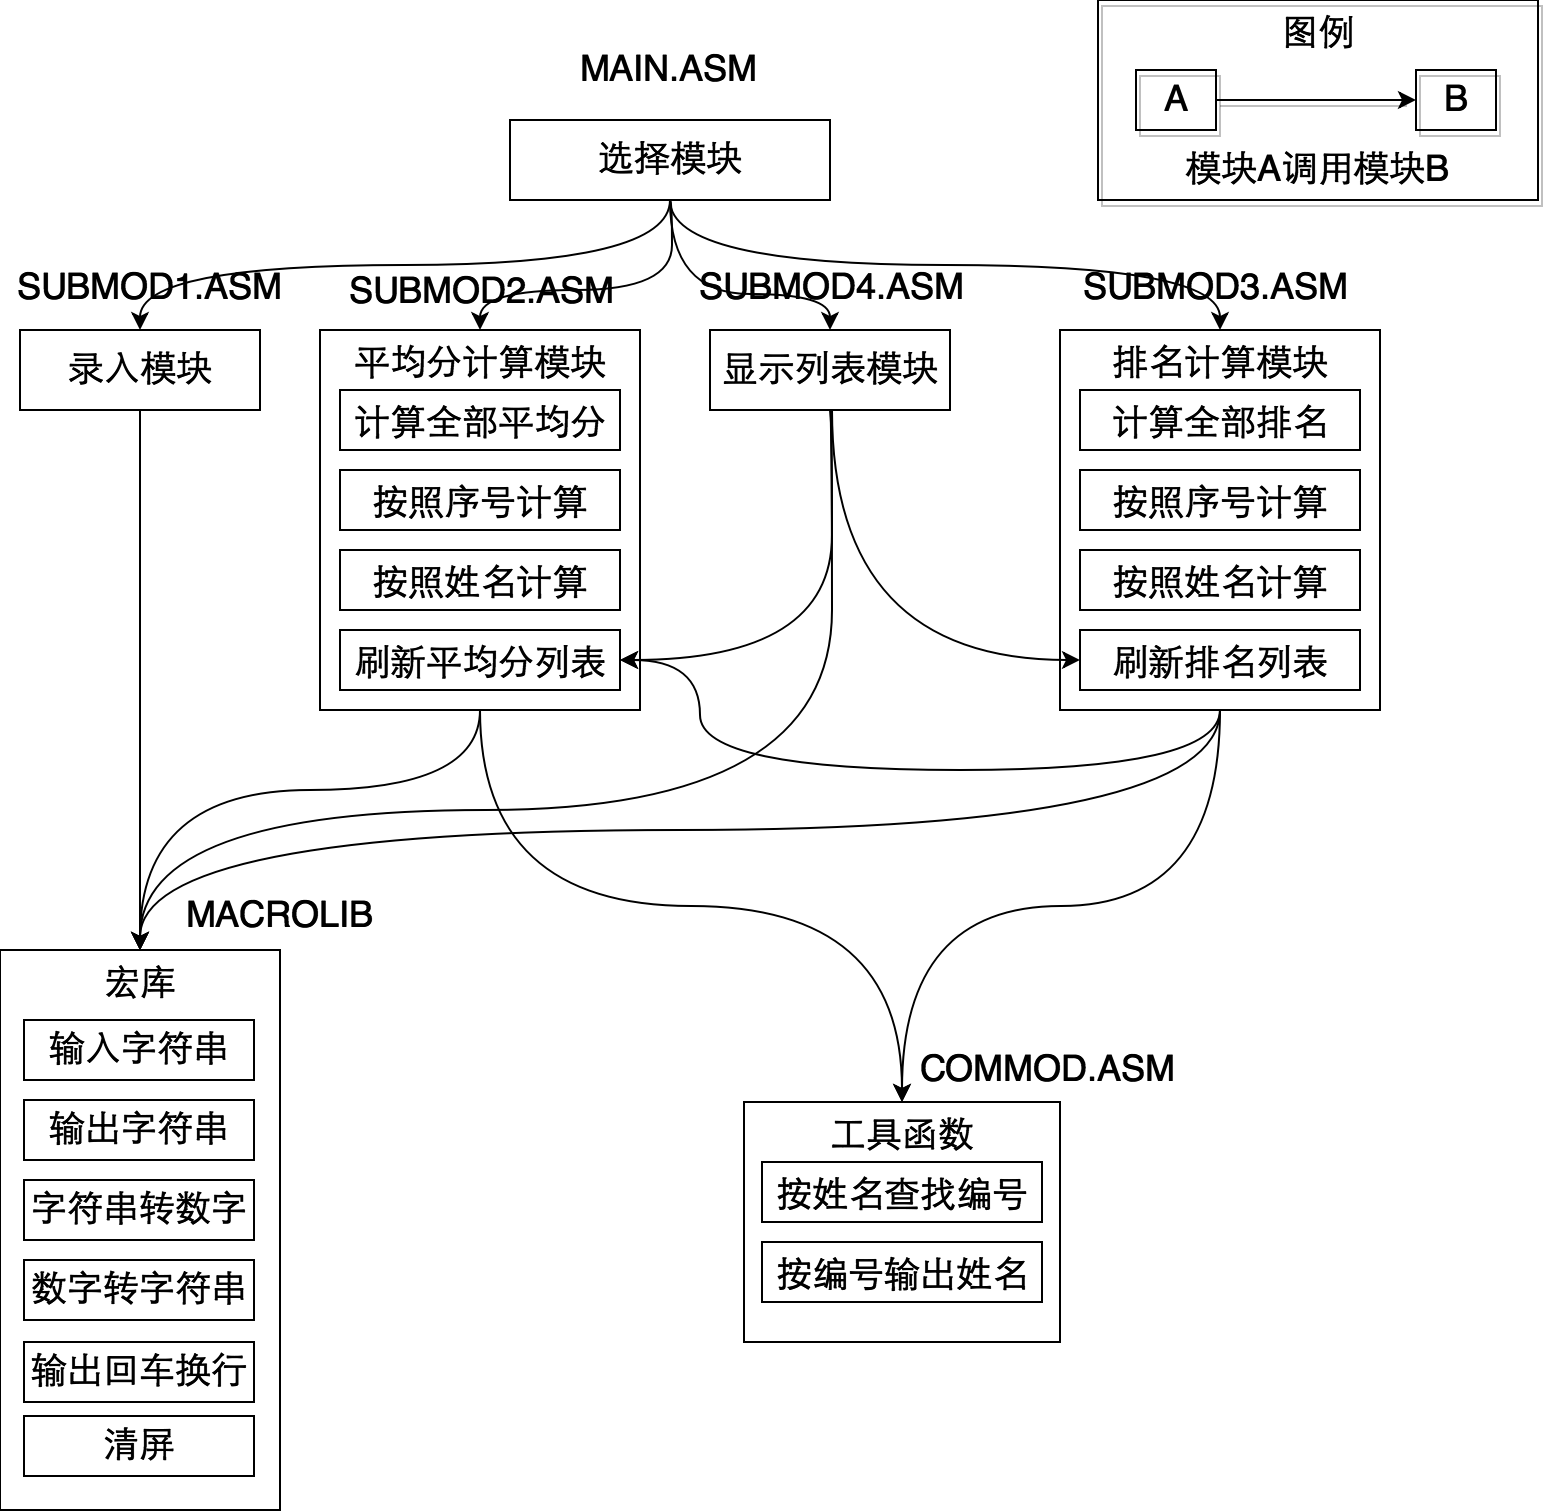
\includegraphics[width=1.0\linewidth]{res/homework_3/module.png}
		\caption{学生成绩管理系统模块调用图}
		\label{fig:module}
	\end{figure}

	\begin{figure}[H]
		\centering
		\includegraphics[width=0.8\linewidth]{res/homework_3/flow_main.png}
		\caption{学生成绩管理系统总体模块流程图}
		\label{fig:flowm}
	\end{figure}

	\begin{multicols}{2}
		\begin{figure}[H]
			\centering
			\includegraphics[height=0.4\textheight]{res/homework_3/flow_1.png}
			\caption{录入模块流程图}
			\label{fig:flow1}
		\end{figure}

		\begin{figure}[H]
			\centering
			\includegraphics[height=0.4\textheight]{res/homework_3/flow_4.png}
			\caption{显示输出模块流程图}
			\label{fig:flow4}
		\end{figure}
	\end{multicols}

	\begin{figure}[H]
		\centering
		\includegraphics[height=0.45\textheight]{res/homework_3/flow_2.png}
		\caption{平均分计算模块流程图}
		\label{fig:flow2}
	\end{figure}

	\begin{figure}[H]
		\centering
		\includegraphics[height=0.45\textheight]{res/homework_3/flow_3.png}
		\caption{排名计算模块流程图}
		\label{fig:flow3}
	\end{figure}

	\subsubsection{源程序}
	源程序分为8个文件:
	\begin{enumerate}
		\item 主程序(菜单选择及模块调用)--- MAIN.ASM
		\item 录入模块 --- SUBMOD1.ASM
		\item 平均分计算模块 --- SUBMOD2.ASM
		\item 排名计算模块 --- SUBMOD3.ASM
		\item 成绩单输出模块 --- SUBMOD4.ASM
		\item 宏库 --- MACROLIB
		\item 工具函数模块 --- COMMOD.ASM
		\item nmake文件 --- MAKEFILE
	\end{enumerate}
	由于源程序较长,为不影响排版,详细源程序请见附录部分。(第\pageref{code:3_1}页)

	\subsubsection{实验步骤}
	\begin{enumerate}
		\item 按照模块编写程序,并分别编译各个模块。若编译出错,则分别修改每一个模块中的错误,直到所有模块都能够通过编译。
		\item 链接各个模块,依照连接过程中可能出现的错误信息重新修改、编译、链接程序。
		\item 直接运行程序,测试所有功能,观察有无错误产生。若有,则重复修改,并执行nmake。
		\item 在功能测试的过程中,需要加入可能出现的非法输入,测试程序在应对错误的输入时是否能正常处理。
		\item 由于直接运行程序不能观察到程序的内部运行状况,打开调试器调试程序:
		\begin{enumerate}
			\item 首先观察程序编译后的状况,包括不同文件的合并方式、段的位置、宏展开的情况、子程序调用传参等情况等。
			\item 在程序的关键位置(输入输出、子程序调用、宏展开等)打上断点,并运行程序,动态的观察在程序运行的过程中是如何处理程序的调用、外部符号等。
		\end{enumerate}
	\end{enumerate}


	\subsubsection{实验记录与分析}

	\begin{enumerate}
		\item 实验环境条件:i7 3.6GHz,8G内存;Archlinux下DOSBox0.74; VIM.EXE 7.3; TASM 5.0、TLINK 5.0、TD 5.0编译、链接、调试套件,使用nmake1.20管理编译与链接。
		\item 按设计思想编写源文件,进行编译,并进行运行测试,根据所出现的错误重复修改、编译连接、运行的过程。在此过程中,主要出现过以下错误:
			\begin{enumerate}
				\item 将extrn输入为extern, TASM 不能正确识别。
				\item 在调用宏的时候参数为带有offset的两个单词,但是没有加上尖括号。
				\item 使用masm的进行编译时候extern符号后没有加入byte、near、abs等修饰符会被识别为错误,但使用TASM编译则不会。
				\item 将equ宏前面加上了word ptr, 导致立即数被当成指针处理,进行了寻址
				\item 在进行录入操作的时候, 没有清空上一次录入的缓冲区,导致录入不正确。
				\item 在进行字乘法运算过程中,由于dx存放结果的高位,但再次之前又将其作为计数器使用并且未进行压栈保护,因此出错。
			\end{enumerate}
		\item 直接运行程序,程序正常运行,并弹出主菜单,如图\ref{fig:mainmenu}所示
			\begin{figure}[H]
				\centering
				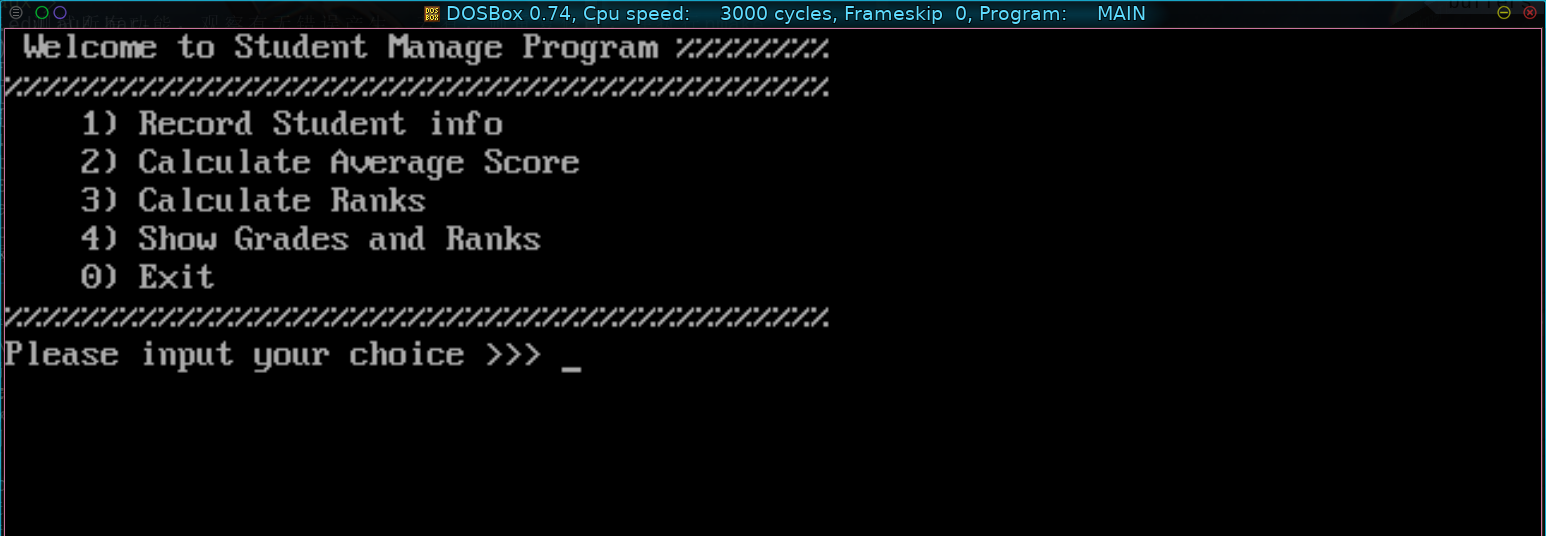
\includegraphics[width=0.8\linewidth]{res/homework_3/mainmenu.png}
				\caption{程序运行主菜单}
				\label{fig:mainmenu}
			\end{figure}
		\item 录入部分学生及其成绩,学生及成绩如表\ref{tab:studentinfo}所示。
			\begin{table}[H]
				\centering
				\caption{录入学生编号、姓名、成绩}
				\label{tab:studentinfo}
				\begin{tabular}{c l l l l c c}
					\toprule
					索引 & 姓名 & 语文成绩 & 数学成绩 & 英语成绩 & 预期平均分 & 预期排名 \\
					\cmidrule(lr){1-1} \cmidrule(lr){2-2} \cmidrule(lr){3-5} \cmidrule(lr){6-6} \cmidrule(lr){7-7}
					0 & alpha	& 95	& 96 & 97	& 95.6 & 3\\
					1 & beta	& 80	& 90 & 100	& 85.7 & 4\\
					2 & gamma	& 100	& 95 & 100	& 98.6 & 1\\
					3 & delta	& 60	& 65 & 66	& 62.3 & 6\\
					4 & epsilon	& 50	& 97 & 86	& 68.6 & 5\\
					6 & Sixu Hu	& 98	& 99 & 88	& 96.9 & 2\\
					\bottomrule
				\end{tabular}
			\end{table}
		\item 直接选择选项4,显示模块会调用平均分计算模块和排名模块的子模块,因此相当于直接测试了三个模块的功能,输出结果如图\ref{fig:tableoutput}所示。可以看出,计算所得结果与预想一致。
			\begin{figure}[H]
				\centering
				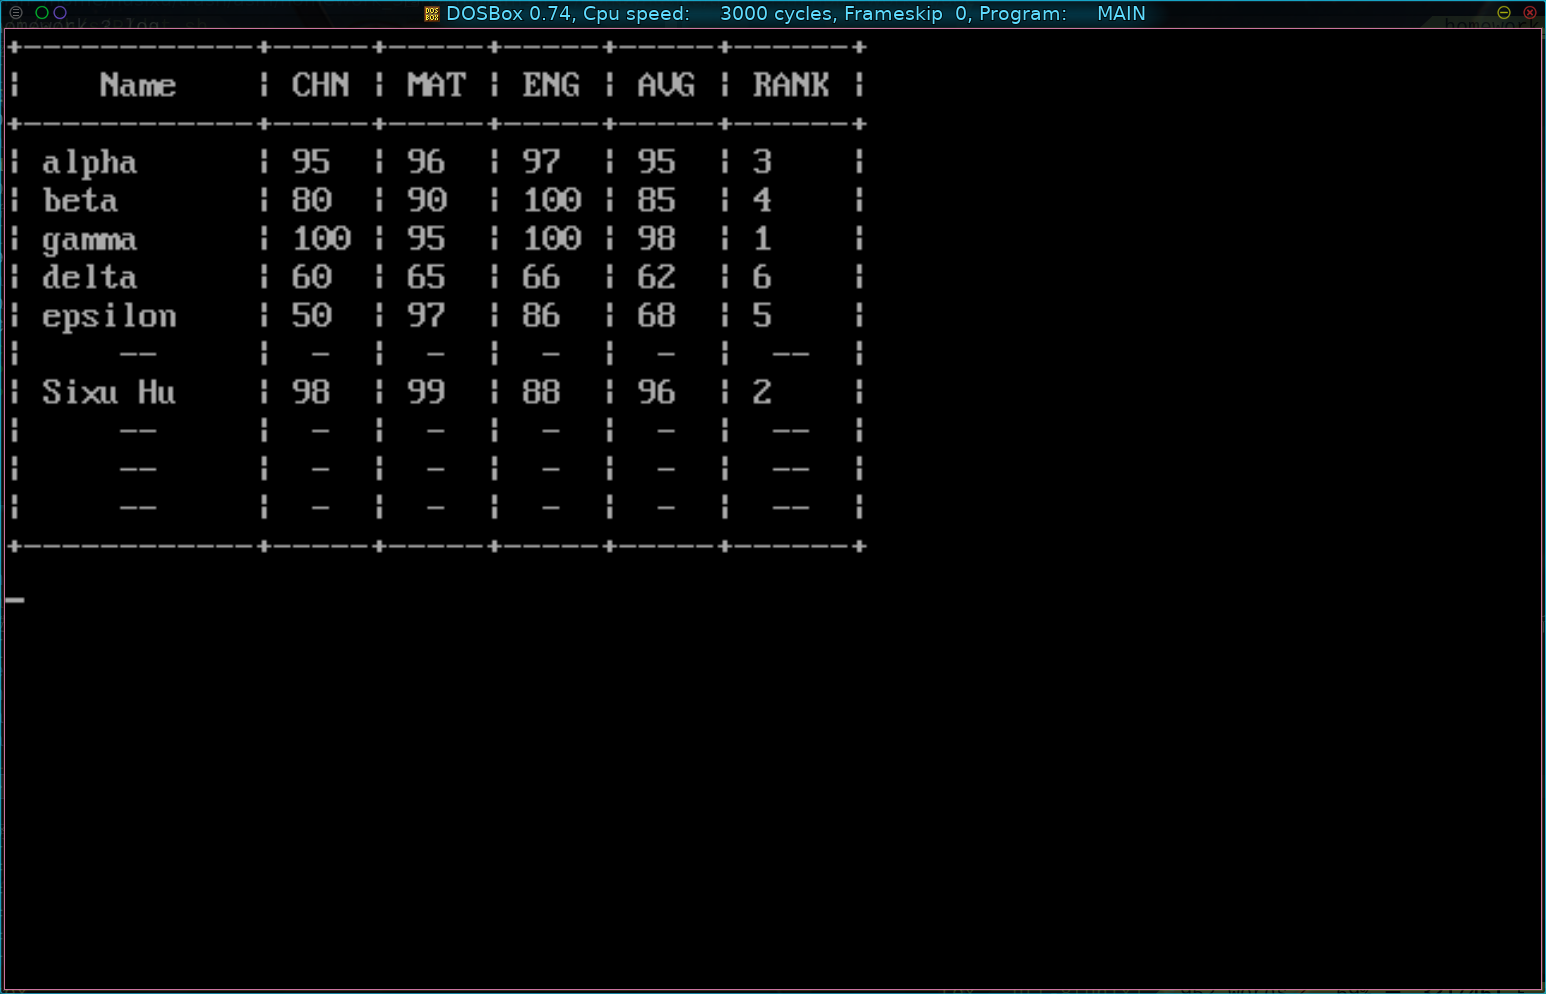
\includegraphics[width=0.8\linewidth]{res/homework_3/tableoutput.png}
				\caption{显示模块输出结果}
				\label{fig:tableoutput}
			\end{figure}
		\item 打开Turbo Debugger,装载程序进行调试,可以观察到,各个模块间的链接方式就是按照tlink的顺序进行的,而程序段间会有少于15个字节的空间(\ref{fig:emptysegment}),以保证段的起始地址能被16整除,说明TASM默认选择PARA作为段的组合方式。
			\begin{figure}[H]
				\centering
				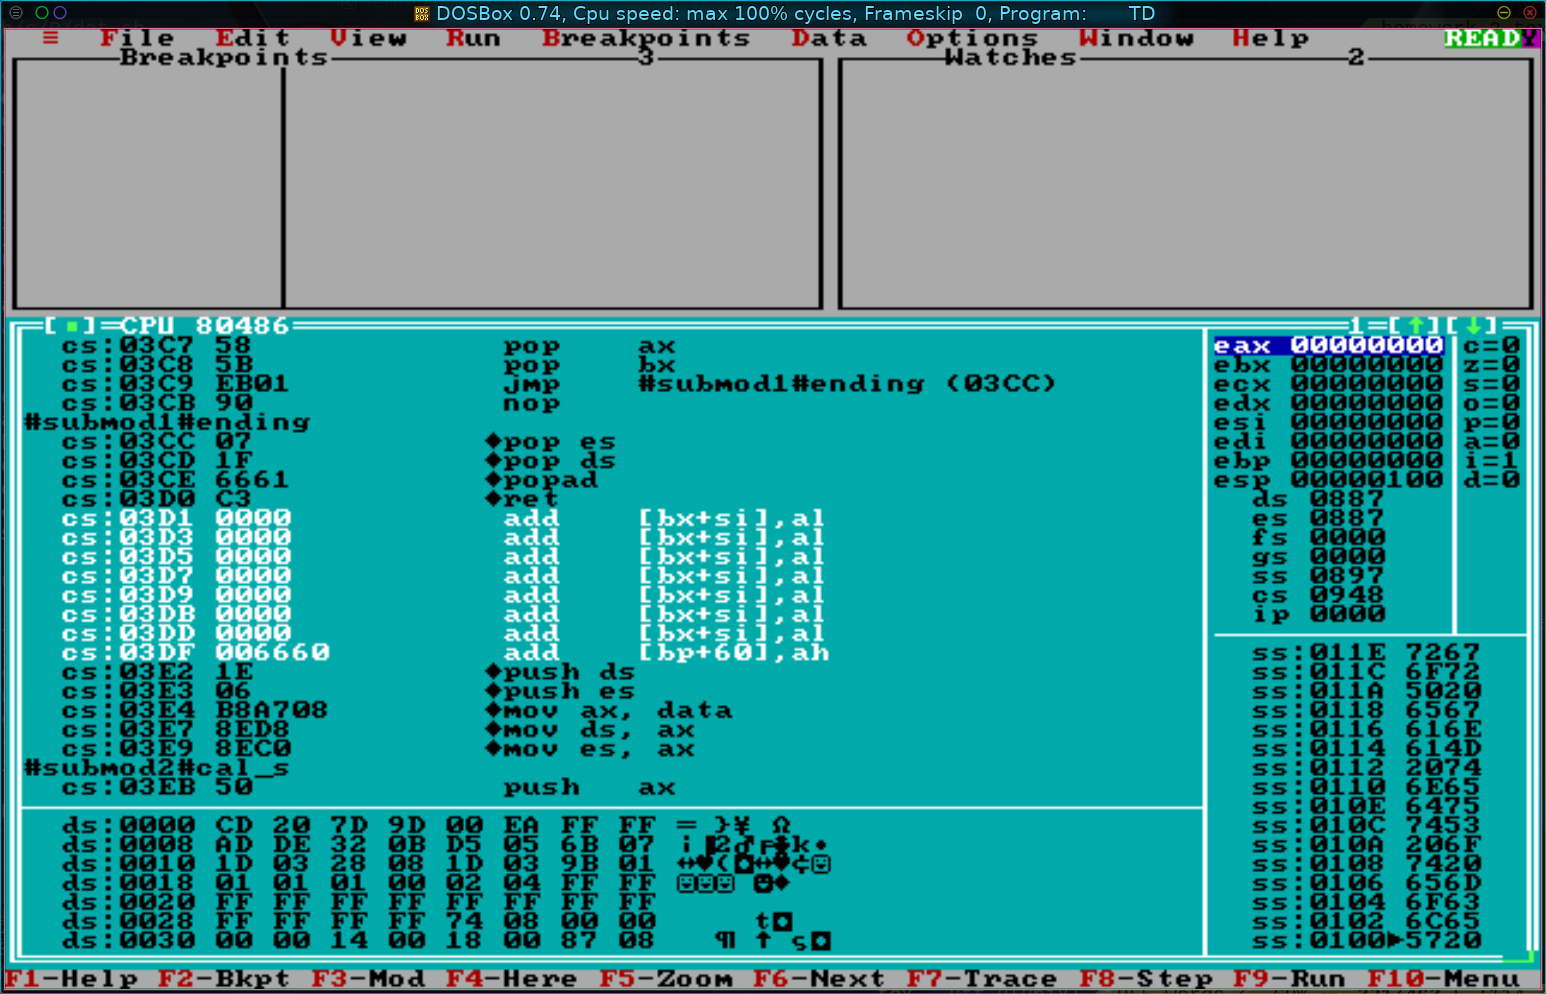
\includegraphics[width=0.8\linewidth]{res/homework_3/emptysegment.png}
				\caption{段之间的空白部分}
				\label{fig:emptysegment}
			\end{figure}
		\item 对于不同段内的相同标号,连接器是这样处理的:在每个标号前加上{\textbf{\#段名\#}},由于段名不会重复,因此所有的标号也会是不同的。
		\item 而对于内嵌于程序段中的宏,编译器是这样处理的:
			\begin{itemize}
				\item 对于宏内的语句直接展开,对于宏内的参数,若不是局部符号,则直接替换。
				\item 对于宏内的局部符号,在一个段内从0开始依次此编号,编号格式为{\textbf{\#段名\#??编号}},在一个段内,只要出现了包含有私有符号的宏就对此私有符号依次进行编号,通过特殊符号(问号)和全局的顺序编号来保证每一个标号的不同。
			\end{itemize}
		\item 在函数传参方面,程序编写时均使用的为堆栈传递参数,在子程序使用参数是要注意保护现场所使用的栈空间,以便于正确的取得参数。若需要返回的值所占用的空间大于传入的参数,则需要先分配好栈空间(通过重复压入需要保护的寄存器)再保护现场。在进行近调用时,存储IP消耗2字节,而进行远调用时,存储CS:IP占用4字节,在函数调用时也需注意。在本程序的测试过程中就因为忽略了原调用和近调用压栈数目不同而导致取得和返回了错误的参数。
		\item 同时,我观察到使用调用时子程序的ret语句被翻译为retf,而近调用则被翻译为ret,这是由于返回时需要弹出不同数量的栈元素所造成的。
	\end{enumerate}


	\subsection{任务二}
	\subsubsection{设计思想}
	除了将输入与输出部分改造为C语言实现外,其余部分均保留为汇编实现,这就需要汇编与C语言互相调用。其中,选择部分调用各个模块为C语言调用汇编,而汇编进行显示输出则为汇编调用C语言。\par
	编写程序时,首先需要了解在相应的编译环境下的C语言与汇编互相调用的方法,然后将MAIN.ASM改为MAIN.C并用C语言实现,将MACROLIB也改为使用C语言实现。对于其余的文件进行必要的更改,以保证能够同时正常工作。

	\subsubsection{模块关系图}
	除了选择菜单与输入输出使用C语言实现外,其余部分均与任务一相同。具体见图\ref{fig:cmodule}
	\begin{figure}[H]
		\centering
		\includegraphics[width=0.8\linewidth]{res/homework_3/cmodule.png}
		\caption{替换后的模块关系调用图}
		\label{fig:cmodule}
	\end{figure}

	\subsubsection{源程序}
	源程序分为8个文件:
	\begin{enumerate}
		\item 主程序(菜单选择及模块调用)--- MAIN.C
		\item 录入模块 --- SUBMOD1.ASM
		\item 平均分计算模块 --- SUBMOD2.ASM
		\item 排名计算模块 --- SUBMOD3.ASM
		\item 成绩单输出模块 --- SUBMOD4.ASM
		\item 宏库 --- MACROLIB
		\item 工具函数模块 --- COMMOD.ASM
		\item nmake文件 --- MAKEFILE
	\end{enumerate} \par
	其中录入模块,平均分计算模块,排名计算模块,成绩单输出模块,工具函数模块与任务一基本相同,除了段的属性与名字,子过程的名字有所更改外,其余部分不变,以diff的形式在附录中给出。而重新使用C语言编写的部分(主程序、宏库、MAKEFILE)则在附录(\pageref{code:3_2})中完整给出。

	\subsubsection{实验步骤}
	\begin{enumerate}
		\item 将任务一中的主函数与工具函数库更改为使用C语言实现,并分别编译各个模块。若编译出错,则分别修改每一个模块中的错误,直到所有模块都通过编译。
		\item 链接各个模块,依照连接过程中可能出现的错误信息重新修改、编译、链接程序。
		\item 依照任务一的方法对与程序进行测试,观察程序是否能够正常运行。
		\item 由于直接执行程序不能看到编译器对于C语言与汇编语言的处理情况,因此使用TD进行调试,主要观察以下几项:
			\begin{itemize}
				\item C语言对于段符号,函数符号等符号的处理规则。
				\item C语言调用C语言函数的参数传递方式
				\item C语言函数调用的参数清理方式
				\item 混合编译后段之间的关系
				\item 汇编语言调用C语言和C语言调用汇编语言的细节
			\end{itemize}
	\end{enumerate}

	\subsubsection{实验记录与分析}
	\begin{enumerate}
		\item 实验环境条件:i7 3.6GHz,8G内存;Archlinux下DOSBox0.74; VIM.EXE 7.3; 直接使用BCC3.0进行编译与链接,TASM3.0进行辅助汇编,使用nmake1.20管理编译与链接。

		\item 在尝试编译的过程中,遇到了许多错误,其中主要的错误如下:
			\begin{itemize}
				\item 使用 bcc 生成main.obj, tasm 生成汇编obj,bcc进行链接:出现错误undefined symbol \_<symbol>,其中<symbol>是汇编过程名,未能正确识别汇编过程。
				\item 使用 bcc 生成main.obj, tasm 生成汇编obj,tlink进行链接:出现错误undefined symbol \_<symbol>,其中<symbol>是标准库中的函数名,如printf等,没有对标准库进行链接。
				\item 使用 bcc 生成main.asm, tasm main.obj以及其他汇编obj, tlink链接:出现错误c0.asm:undefined refrence main,未能正确识别C语言的main函数入口。
				\item 使用 bcc 直接编译链接所有文件生成exe,将汇编文件的model改为C,汇编过程名前不加下划线,生成成功,但不能正确运行。反汇编表明生成的可执行文件对于汇编语言的翻译不正确。 fixup overflow
				\item 使用 bc.exe建立project,并添加C语言和汇编语言文件进行生成:出现错误32-bit record in asm file,而在bc的链接器选项中没有对32位支持的选项,故不能正确识别如eax的32为寄存器名。
			\end{itemize}

		\item 最后通过bcc -3 -v -c -S MAIN.C生成MAIN.ASM,并对MAIN.ASM进行研究后发现,在进行处理时,C语言文件的函数体部分均在\_TEXT段内,数据均在\_DATA段内,并且函数名前都被加上下划线。因此对asm文件进行相似的处理,成功生成exe文件,并可以正常执行,具体进行的处理如下:
			\begin{itemize}
				\item 代码段的段定义改为\_TEXT segment use16 public "CODE"
				\item 数据段的段定义改为\_DATA segment use16 public "DATA"
				\item 在需要被C语言调用的过程名前加下划线
				\item 在C语言调用汇编函数前先声明extern int <procname>(<parameters>);
				\item 在汇编调用C函数前先声明extrn \_<funcnme>:near
				\item \textit{不需要}在汇编文件前使用.MODEL说明模式。
				\item 直接使用bcc编译连接所有的文件,命令及参数为bcc -3 -v -l3 -lv -Tla -e<output> <file\_1>.c <file\_2>.asm ... <file\_n>.asm,其中output为输出文件名,<file\_\textit{x}>.c 和 <file\_\textit{x}>.asm为需要编译的文件。
			\end{itemize}

		\item 在运行时又遇到部分问题,经过不断修改源代码最终可以正常运行并达到于任务一相同的效果,其中出现的问题如下:
			\begin{itemize}
				\item 反汇编表明,在C语言生成的代码中进入函数后会有enter指令,在函数返回前会有leave指令,它们都会影响栈空间的分配,其中enter会压入两个字节到栈中,leave会从栈中弹出两个字节。
				\item 在本编译条件下,C语言调用函数时不会对寄存器做出保护,因此从汇编中调用C语言函数时要先对寄存器进行保护。
				\item C语言参数传递默认是从右向左压栈,并由调用者清理栈中的参数,也就是说,在本编译条件下,函数的调用默然采用cdcel(C Declaration)的形式。因此,在汇编调用C语言的过程中要注意清理栈中的参数。
				\item C语言的代码在显示输出是默认使用第0页,显示模式03作为显示输出\footnote{INT 10H. (2017). En.wikipedia.org. Retrieved 9 April 2017, from https://en.wikipedia.org/wiki/INT\_10H}
			\end{itemize}

		\item 最终程序可正常运行。按照任务一的方式对其进行测试,测试结果表明程序可以正常运行,其功能与任务一相同。
		\item 打开TD进行调试如图\ref{fig:deasm}所示,可以看出,进入主函数前,有enter语句,且C语言的getchar()函数是由fgetc实现的。在需要传参的函数调用后均有pop cx语句,说明栈中的参数是由调用者进行清理的。函数名前均有下划线。
			\begin{figure}[h]
				\centering
				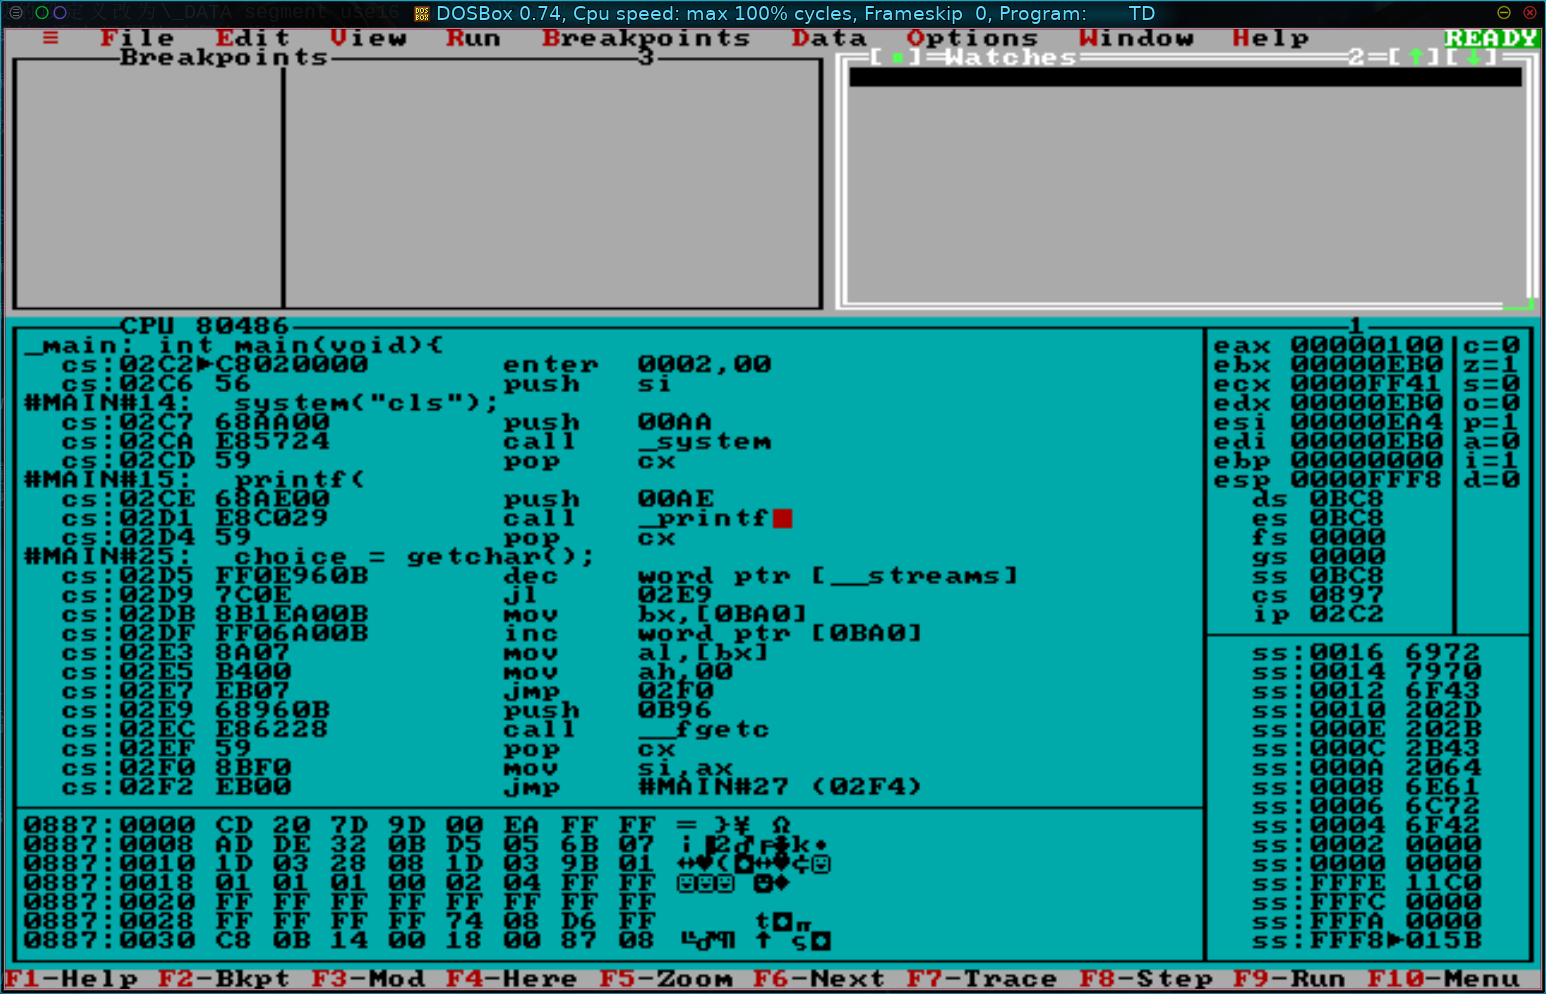
\includegraphics[width=0.9\linewidth]{res/homework_3/deasm.png}
				\caption{对程序进行调试}
				\label{fig:deasm}
			\end{figure}
		\item 在汇编函数调用C函数的时候,需要模仿编译器对于C语言函数的处理:函数名前加下划线,并对调用后的栈空间进行清理。
	\end{enumerate}

	\section{总结与体会}
	通过这次实验,我掌握了子程序设计的方法与技巧,宏指令、模块化程序的设计方法,较大规模程序的合作开发与调试方法,以及C语言与汇编语言混合编译的一些细节问题。\par
	通过实验一,我深刻的体会到了将一个程序分为多个模块的优越性。他不仅使程序编写的逻辑更为清晰,调试更为方便,可以快速缩小调试范围,而且模块化的程序编写更适合多人合作开发,加速了开发的过程。此外,通过这一次实验,我了解到了模块化汇编中的一些细节问题。如在模块间的程序调用时,需要考虑参数的存放位置,特别是在堆栈中存放参数的时候,需要考虑子程序类型(near、far)对参数位置的影响。此外我还观察到编译器对于一些符号的处理,比如不同模块中的同名符号和宏汇编中的局部变量等等,汇编器的处理使他们不会产生冲突,但是需要对于外部符号进行引用的时候,需要先声明才可以引用,否则编译器会产生错误。\par
	使用宏汇编和子过程时,我将其进行了比较,发现他们有相同之处,即都提高了代码的复用率,但是也有其各自的优缺点:宏汇编虽然使用较为简单,参数的传递方式也更为清晰,但是编译后会在每一处展开,不仅占用了空间,如果频繁使用,在调试时也会影响可读性;而子过程则较为节省空间,但需要考虑段转移带来的影响以及参数传递的方式,使用堆栈进行传参和返回时需要仔细的计算,否则参数的位置容易出错。\par
	而实验二使我明白了不同也语言是可以协同解决同一个问题的,并且正确的混合使用不同的语言可以利用到每个语言的优势。\par
	在实验二刚开始进行的时候我面对了不小的挑战:不论怎样替换操作系统、编译工具和源代码总是不能编译成功,或者变异成功后不能得到正确的可执行文件。但当我将C语言文件用编译器生成汇编病仔细的分析过后终于发现了问题的所在和解决的方法,同时也对编译器的行为有了更深的了解。而在能够正确编译后,为了使程序正常运行,我又岁程序进行了漫长的调试。在这个过程中,我对混合调试以及C语言和汇编之间的关系有了更深一层的认识。 \par
	总体而言,这次实验使我收获颇丰,在实验中所学到的知识可能会对未来将要进行的程序优化以及调试起到帮助。

%% Part Four %%%%%%%%%%%%
%%%%%%%%%%%%%%%%%%%%%%%%%
\newpage
\part{中断与反跟踪}
	\section{实验目的与要求}
	\begin{enumerate}
		\item 掌握中断矢量表的概念;
		\item 熟悉I/O访问,BIOS功能调用方法;
		\item 掌握实方式下中断处理程序的编制与调试方法;
		\item 熟悉跟踪与反跟踪的技术;
		\item 提升对计算机系统的理解与分析能力。
	\end{enumerate}

	\section{实验内容}
	\subsection[任务一]{任务一:获取中断入口地址}
	用三种方式获取中断类型码21H对应的中断处理程序的入口地址。
	\noindent\textbf{要求:} \par
	首先要进入虚拟机状态,然后:\par
	\begin{enumerate}
		\item 直接运行调试工具(TD.EXE),观察中断矢量表中的信息。
		\item 编写程序,用 DOS系统功能调用方式获取,观察功能调用相应的出口参数与“(1)”看到的结果是否相同 (使用TD观看出口参数即可)。
		\item 编写程序,直接读取相应内存单元,观察读到的数据与“(1)”看到的结果是否相同 (使用TD观看程序的执行结果即可)。
	\end{enumerate}

	\subsection[任务二]{任务二:接管键盘中断}
	编写一个接管键盘中断的中断服务程序并驻留内存,要求在程序返回DOS操作系统后,键盘上的小写字母都变成了大写字母。 \par
	\noindent\textbf{要求:} \par
	\begin{enumerate}
		\item 在 DOS虚拟机或DOS窗口下执行程序,中断服务程序驻留内存。
		\item 在DOS命令行下键入小写字母,屏幕显示为大写,键入大写时不变。执行TD,在代码区输入指令“mov  AX,0”看是否能发生变化。
		\item 选作:另外编写一个中断服务程序的卸载程序,将键盘中断服务程序恢复到原来的状态(也就是还原中断矢量表的信息,先前驻留的程序可以不退出内存)。
	\end{enumerate}

	\subsection[任务三]{任务三:读取CMOS信息}
	读取CMOS内指定单元的信息,按照16进制形式显示在屏幕上。\par
	\noindent\textbf{要求:} \par
	\begin{enumerate}
		\item 先输入待读取的CMOS内部单元的地址编号(可以只处理编号小于10的地址单元)。再使用IN/OUT指令,读取CMOS内的指定单元的信息。
		\item 将读取的信息用16进制的形式显示在屏幕上。若是时间信息,可以人工判断一下是否正确。
	\end{enumerate}

	\subsection[任务四]{任务四:数据加密与反跟踪}
	在实验一的学生成绩查询程序的基础上,增加查询前输入密码的功能,密码不对则程序退出,只有密码正确之后才能完成后续的功能。密码采用密文的方式存放在数据段中。各科成绩也以密文方式存放在数据段中。加密方法自选。\par
	可以采用计时、中断矢量表检查、堆栈检查、间接寻址等方式中的一种或多种方式反跟踪(建议只采用一到两种反跟踪方法,重点是深入理解和运用好所选择的反跟踪方法)。\par
	成绩表中要有编程者自己的名字(姓的全拼+名字的拼音首字母,但大小写可以随意组合)和各科成绩(姓名和成绩都密文存放)。成绩表中只需要定义三个学生的信息即可。
	\textbf{提示:}为了使源程序的数据段中定义的密码、学生姓名、各科成绩能在汇编之后变成密文(也就是在最后交付出去的执行程序中看不到明文),可以使用数值运算符(参见教材P48)对变量的初始值进行变换。例如,如果想使语文成绩90分变成密文,加密算法是与密钥字符“W”做异或运算,则可写成:
	\begin{codeFont}
		\begin{lstlisting}[gobble=12]
			YUWEN     DB  90  XOR  ‘W
		\end{lstlisting}
	\end{codeFont}

	\subsection[任务五]{任务五:跟踪与数据解密}
	解密同组同学的加密程序,获取该同学的各科成绩。\par
	\textbf{注意:}两人一组,每人实现一套自己选择的加密与反跟踪方法,把执行程序交给对方解密(解密时间超过半小时的,说明反跟踪方法基本有效)。如何设计反跟踪程序以及如何跟踪破解,是本次实验报告中重点需要突出的内容。(分组可以按照学号顺序依次构成两人一组。也可以自行调整。如果班上人数是奇数,则三人一组,甲解密乙的,乙解密丙的,丙解密甲的)

	\section{实验过程}
	\subsection{任务一}
	\subsubsection{实验步骤}
	\begin{enumerate}
		\item 首先使用第一种方法获得中断入口地址:打开TD直接观察,将int 21H的地址记录下来。
		\item 编写程序,在程序中首先使用系统功能调用的方法,再使用直接读取的方法获得地址。
		\item 编译、链接、调试程序。
		\item 观察并记录程序的运行结果,并与第一种方法获得的结果进行比较。
	\end{enumerate}

	\subsubsection{源程序}
	使用第二种和第三种方法获得中断入口地址的源程序见附录部分(第\pageref{code:4_1}页)

	\subsubsection{实验记录与分析}
	\begin{enumerate}
		\item 实验环境条件:i7 3.6GHz,8G内存;Archlinux下DOSBox0.74; VIM.EXE 7.3; TASM 5.0、TLINK 5.0、TD 5.0编译、链接、调试套件。
		\item 由CPU响应中断的过程可知,int 21H的地址应该存储于$0x21\times4=132(0x84)$处,并占用4个字节,因此在TD中切换到数据显示区,按下Ctrl+G并输入00:84使光标跳转到对应位置,并读出int 21H的地址为IP:01CC CS:031D,如图\ref{fig:int21address}所示。
			\begin{figure}[H]
				\centering
				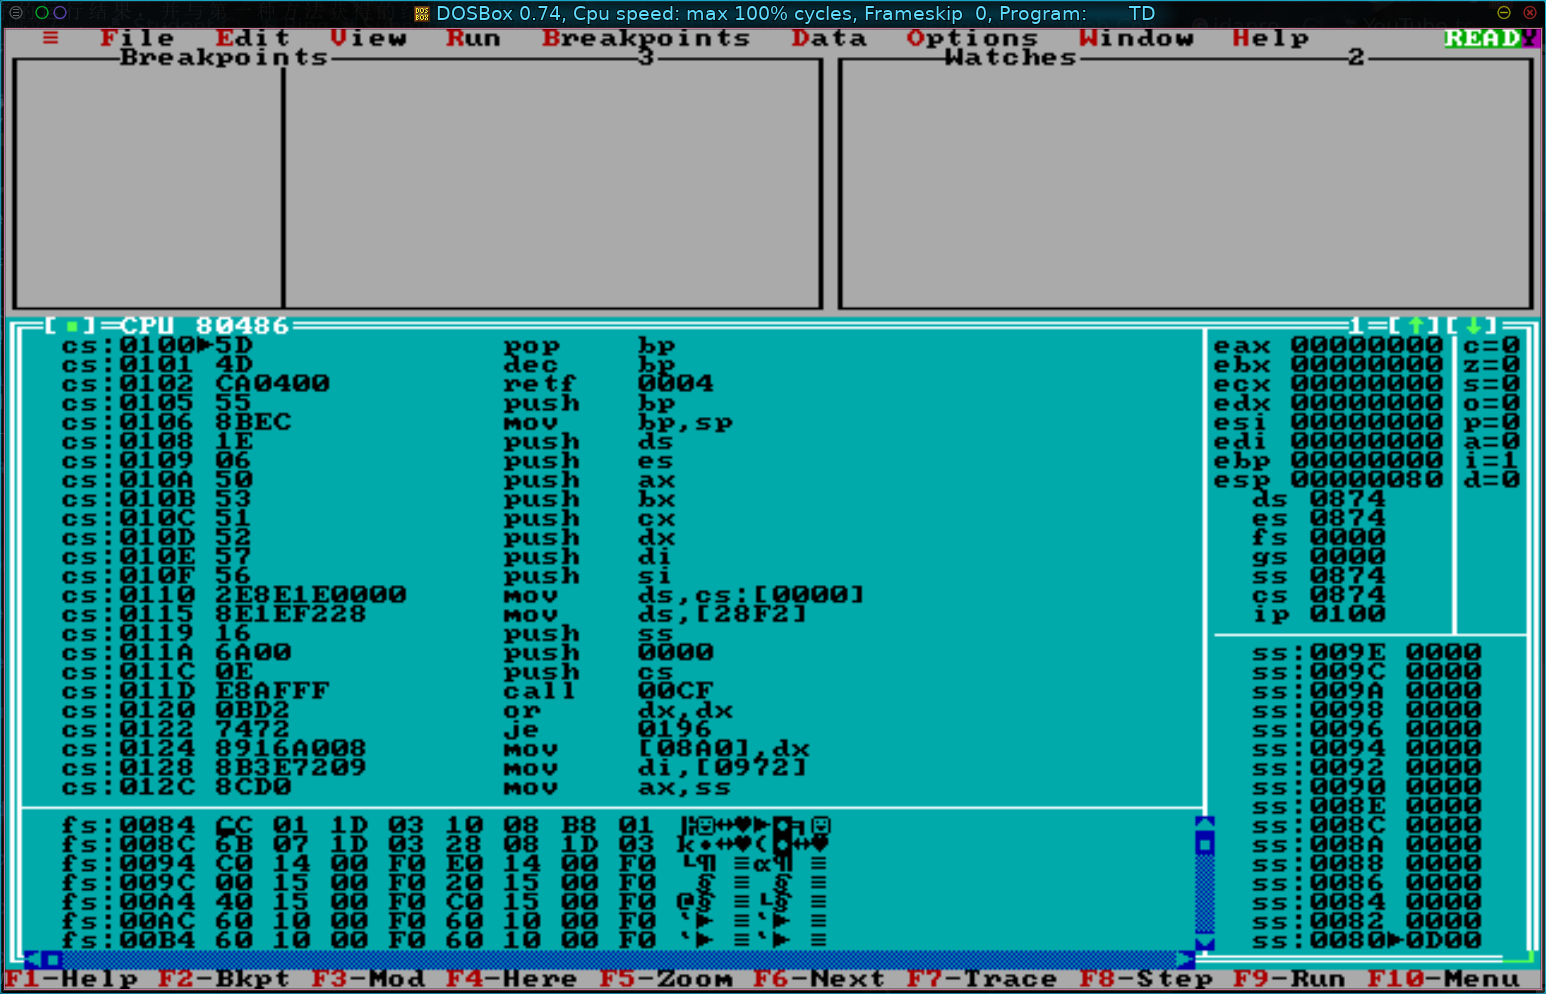
\includegraphics[width=0.9\linewidth]{res/homework_4/int21address.png}
				\caption{从TD中读取的int 21H地址}
				\label{fig:int21address}
			\end{figure}

		\item 编译链接程序,程序并未出错,直接运行程序,结果如图\ref{fig:runprog}所示,IP=5280=14A0H,CS=61440=F000H,结果发现,与在TD中调试的结果并不相同。
			\begin{figure}[H]
				\centering
				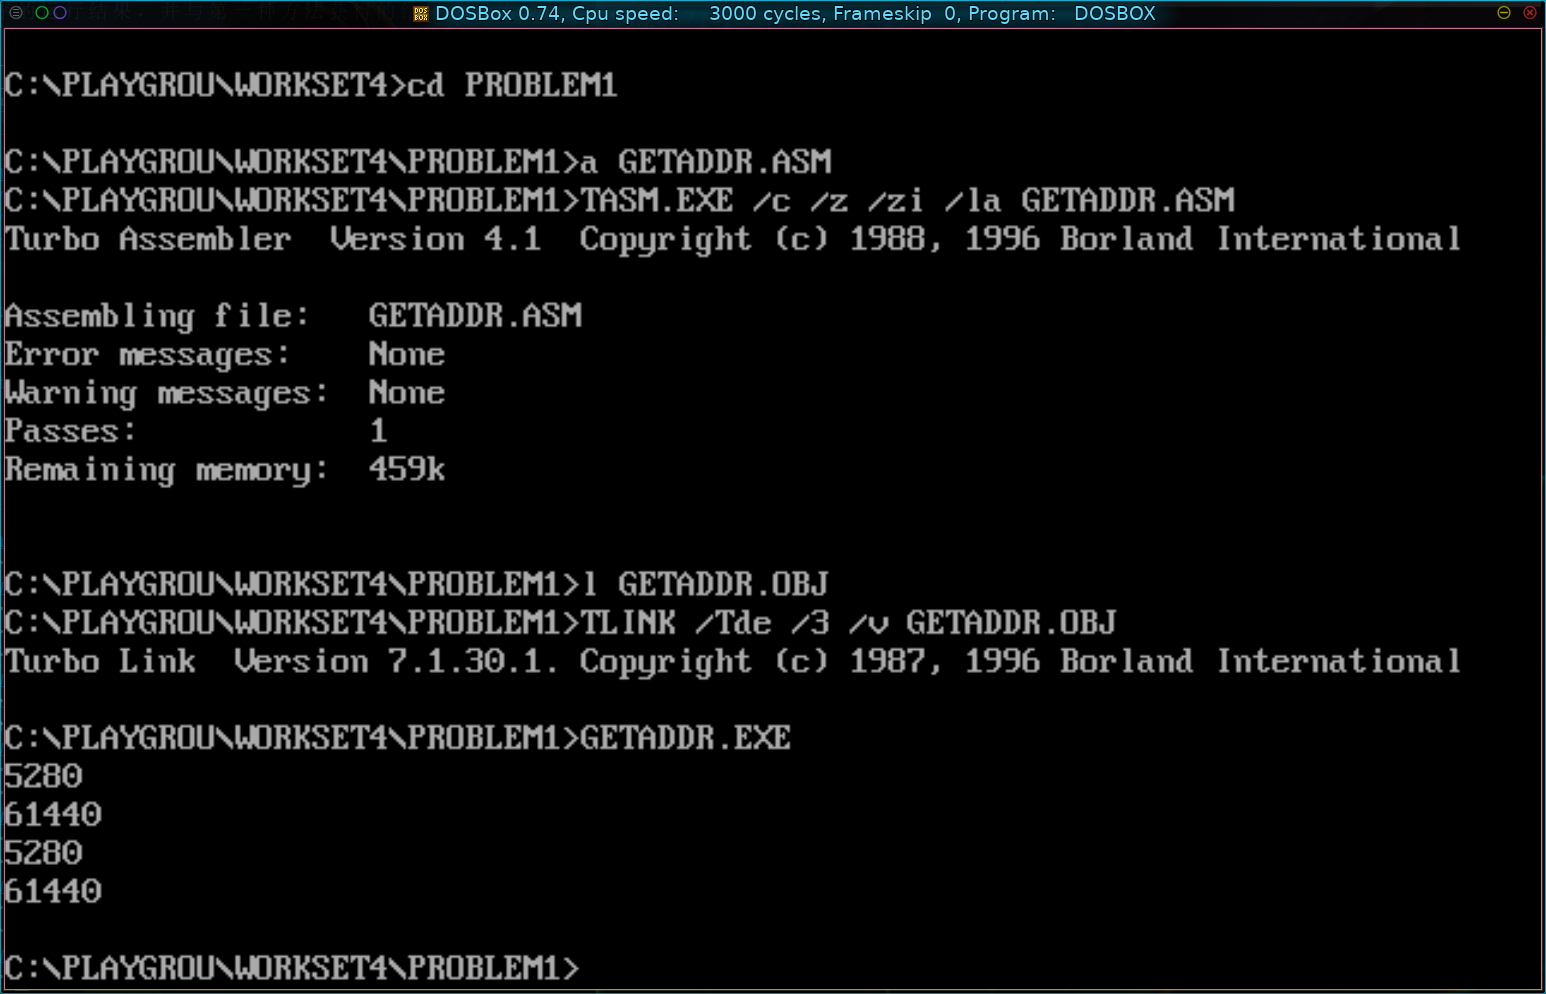
\includegraphics[width=0.9\linewidth]{res/homework_4/runprog.png}
				\caption{直接运行程序结果}
				\label{fig:runprog}
			\end{figure}

		\item 换用int20进行实验,在td中调试的结果如图\ref{fig:int20address}所示,其中IP=1480,CS=F000。
			\begin{figure}[H]
				\centering
				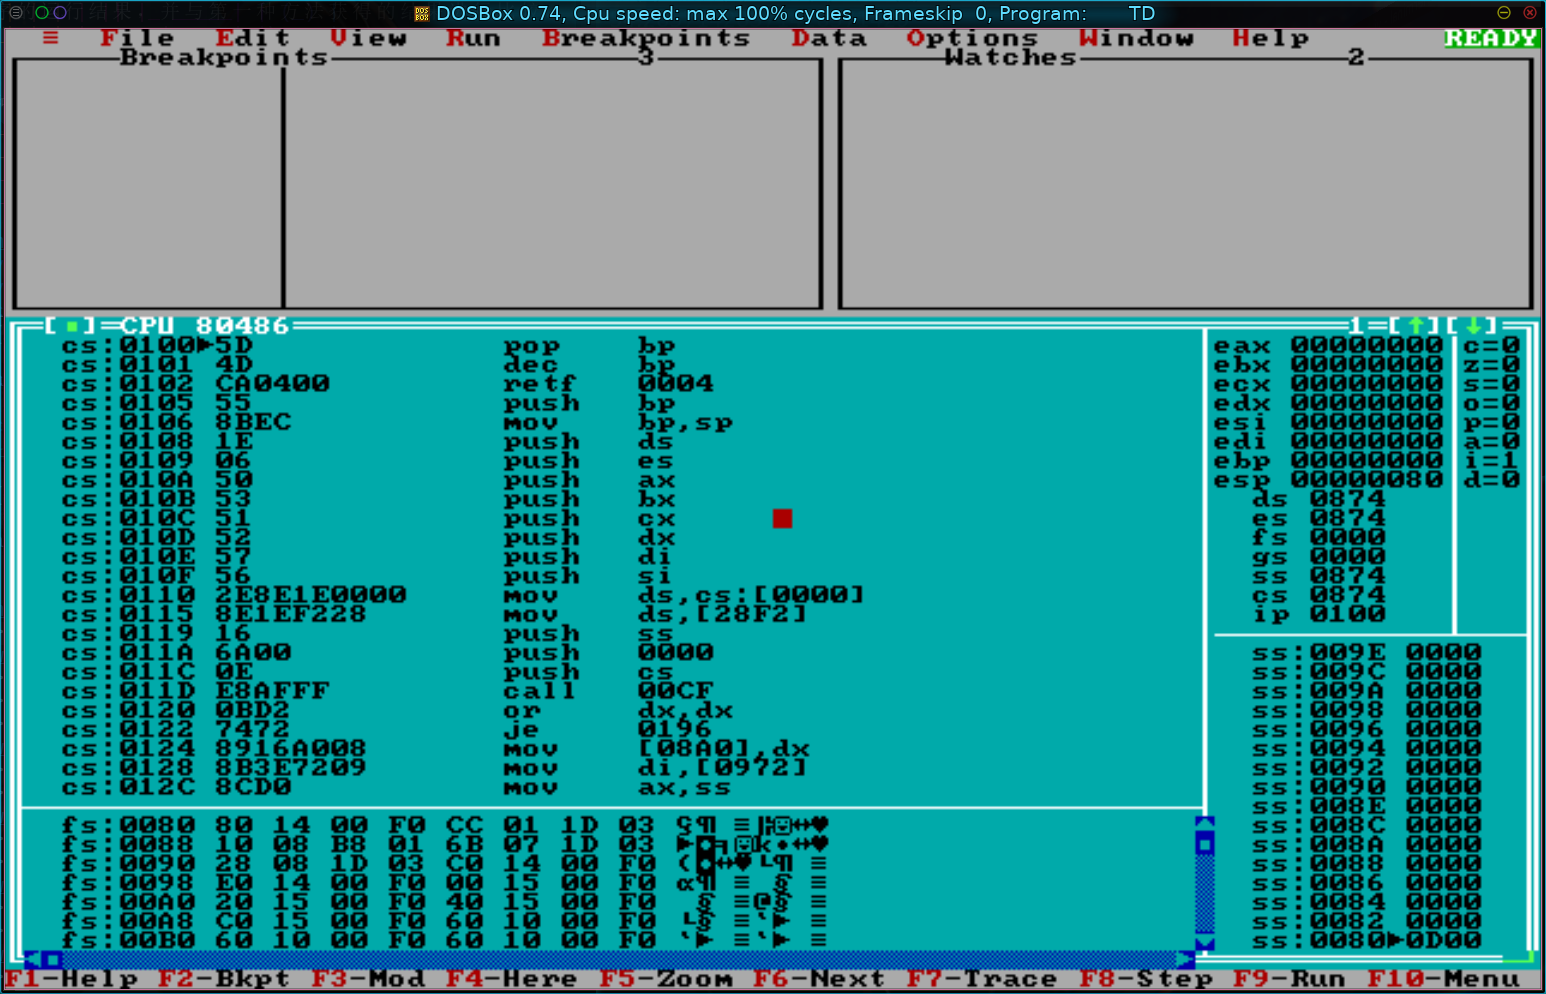
\includegraphics[width=0.9\linewidth]{res/homework_4/int20address.png}
				\caption{从TD中读取的int 20H地址}
				\label{fig:int20address}
			\end{figure}

		\item 修改源程序,使之显示int 20h的入口地址,结果如图\ref{fig:runprog20}所示,其中IP=5248=1480H,CS=61440=F000H,与TD中结果一致。
			\begin{figure}[H]
				\centering
				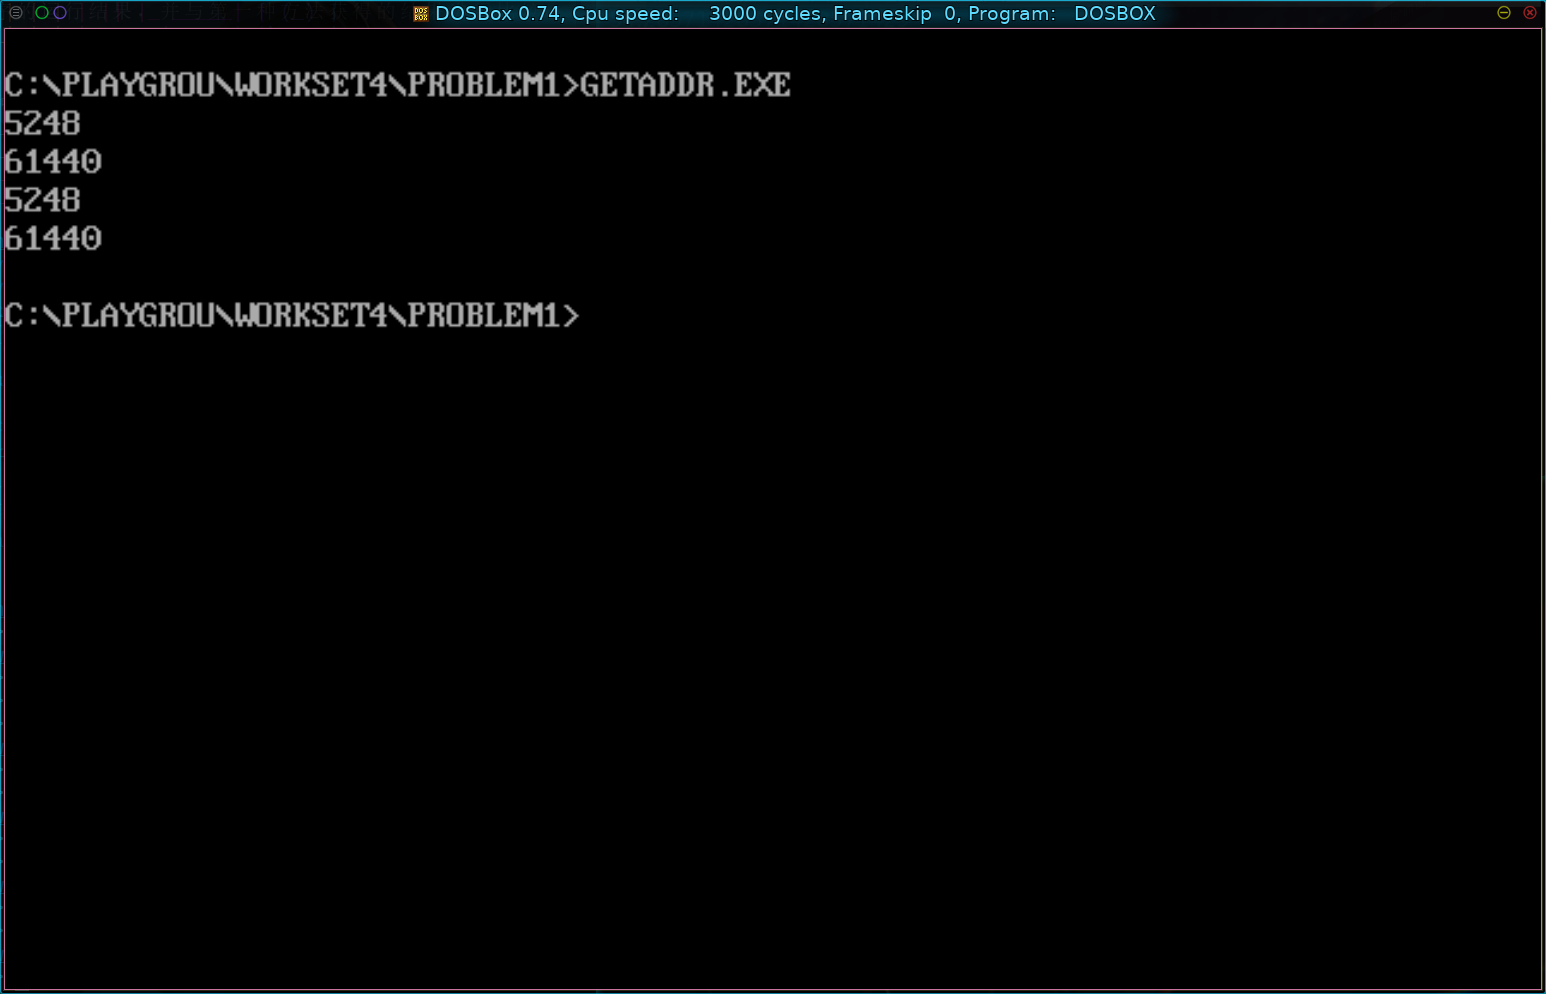
\includegraphics[width=0.9\linewidth]{res/homework_4/runprog20.png}
				\caption{直接运行程序结果}
				\label{fig:runprog20}
			\end{figure}
		\item 由此可知,TD接管了int 21h中断,但是未接管int 20h中断,使用20h号中断验证结果依然正确。
	\end{enumerate}

	\subsection{任务二}
	\subsubsection{设计思想}
	通过将原有的中断替换为新编写的中断,并将原有中断存储起来以供恢复,即可完成中断的接管。在设计新的中断程序时,对于原有的中断不需要修改的部分可以直接调用原有的中断,而对于需要修改的部分可以调用后对结果进行修改,也可以直接编写一个新的中断。

	\subsection{中断地址}
	图\ref{fig:modify}是修改中断时的地址关系,将原来的16h中断保留在60h中断处,然后在16h处加入自己的中断。而图\ref{fig:reset}是将原始的中断恢复的过程,直接将保留的60h处的原始中断地址移动到16h处。\par
	\begin{minipage}{0.59\textwidth}
		\begin{figure}[H]
			\centering
			
\includegraphics[height=0.25\textheight]{res/homework_4/modify.png}
			\caption{修改中断地址}
			\label{fig:modify}
		\end{figure}
	\end{minipage}
	\hfill
	\begin{minipage}{0.39\textwidth}
		\begin{figure}[H]
			\centering
			\includegraphics[width=0.25\textheight]{res/homework_4/reset.png}
			\caption{还原中断地址}
			\label{fig:reset}
		\end{figure}
	\end{minipage}

	\subsubsection{源程序}
	设置中断与恢复中断程序见附录部分(第\ref{code:4_2}页)

	\subsubsection{实验步骤}
	\begin{enumerate}
		\item 按照设计思想编写源程序,注意在设置中断的过程中需要关中断。
		\item 编译、链接,并重复修改源程序,直到没有错误。
		\item 直接运行编译结果SETINT.EXE,观察输入的小写字母是否变为了大写。
		\item 运行编译结果REMOVE.EXE,观察中断是否被还原。
		\item 打开TD调试,观察中断被替换的过程。
	\end{enumerate}

	\subsubsection{实验记录与分析}
	\begin{itemize}
		\item 实验环境条件:i7 3.6GHz,8G内存;Archlinux下DOSBox0.74; VIM.EXE 7.3; TASM 5.0、TLINK 5.0、TD 5.0编译、链接、调试套件。
		\item 在编译与链接的过程中没有出错,但在运行时出现了输入无响应的错误。
		\item 经过对源代码的观察发现,进入中断时使用了PUSHAD,而退出中断前使用了POPAD,导致中断的出口参数丢失。
		\item 将源程序修改后重新编译、连接、运行。程序返回DOS后,发现输入的小写字母均变为了大写字母。
		\item 运行REMOVE.EXE再次输入字母测试,发现输入的字母又还原为小写字母,两次运行的结果如图\ref{fig:runint}所示。
			\begin{figure}[H]
				\centering
				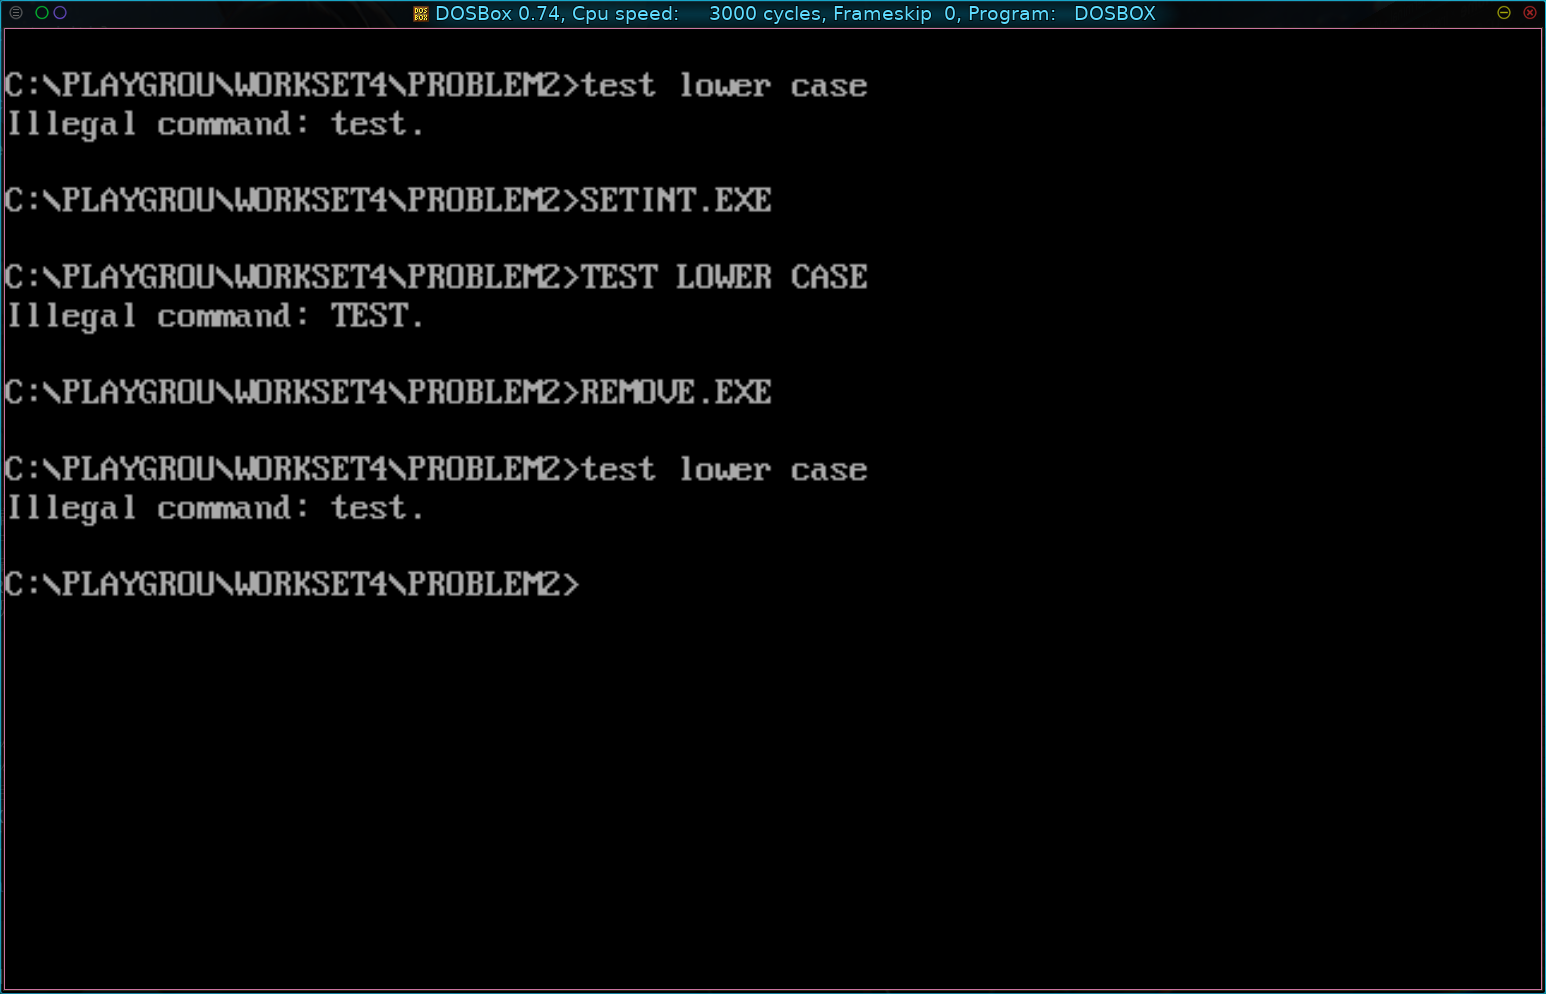
\includegraphics[width=0.8\linewidth]{res/homework_4/runint.png}
				\caption{接管中断与恢复中断}
				\label{fig:runint}
			\end{figure}
		\item
		\item 打开TD,对于源程序进行调试,发现原来的16h中断地址被顺利的00:0180h处,但是00:0058h的值在设置时没有发生变化,在TD中的输入也没有变成大写。猜想TD为了保证在调试时键盘输入不至于被破坏,接管了16h中断或对此中断入口进行了保护。
	\end{itemize}

	\subsection{任务三}

	\subsubsection{设计思想}
	直接使用in和out指令,对于CMOS进行操作。在70h端口写,71h端口读出数据。在程序的编写过程中可以调用实验2宏库中的输入输出及字符串与数字转换的部分。

	\subsubsection{源程序}
	CMOS操作源程序见附录部分(第\pageref{code:4_3}页),其中MACROLB与实验二任务一的MACROLIB相同。

	\subsubsection{实验步骤}
	\begin{itemize}
		\item 编写源程序,请求用户输入,将输入转换为数字后使用in/out指令通过70h/71h端口与CMOS芯片进行交流,并将输出转换为16进制文本输出。
		\item 编译、链接,并重复修改源程序,直到没有错误。
		\item 直接运行源程序,读取年、月、日、时、分、秒等信息,并与计算机信息进行对比,观察是否正确。
	\end{itemize}

	\subsubsection{实验记录与分析}
	\begin{itemize}
		\item 实验环境条件:i7 3.6GHz,8G内存;Archlinux下DOSBox0.74; VIM.EXE 7.3; TASM 5.0、TLINK 5.0、TD 5.0编译、链接、调试套件。
		\item 编写源程序,将in所获得的值\textbf{转换为十进制}输出,并进行编译、链接。在此过程中未出现错误。
		\item 还接运行程序,观察到所获得的时间值与计算机上显示的时间值并不一致,而是将计算机显示时间当做16进制数,转换为10进制的结果。
		\item 修改源程序,将所获得的数字以16进制文本呢的格式进行输出,观察到与计算机显示一致,如图\ref{fig:cmos}所示(右上角为系统时间)
			\begin{figure}[H]
				\centering
				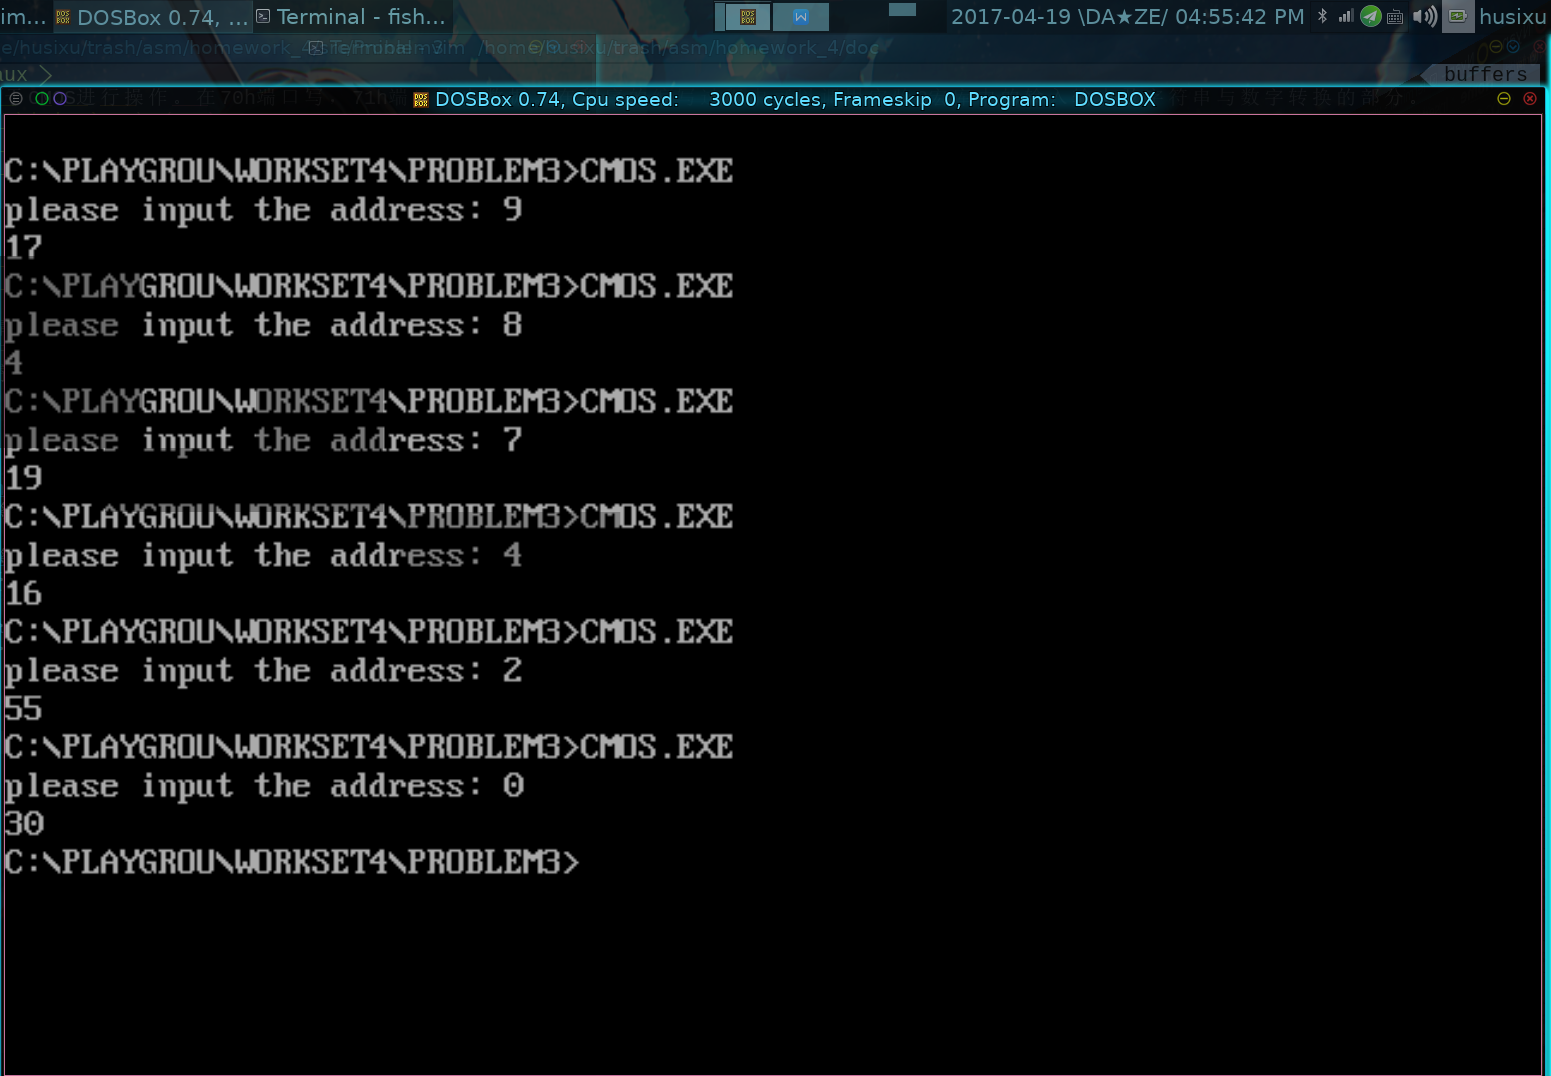
\includegraphics[width=0.95\linewidth]{res/homework_4/cmos.png}
				\caption{读取CMOS显示时间}
				\label{fig:cmos}
			\end{figure}
		\item 从结论可以看出,CMOS中的时间存储的数值为$\frac{time}{10}\times 16+(time\%10)$,其中$time$为时间数值(年、月、日等),直接转换十六进制文本后即为当前时间。
	\end{itemize}

	\subsection{任务四}
	\subsubsection{设计思想}
	使用简单的加密方式对于姓名,分数以及需要输入的密码进行加密,在此基础上使用较为复杂的反跟踪方式进行混淆,从而使加密的步骤难以被识别,达到保护数据的效果。对于本程序而言,采用如图\ref{fig:encrypt}的简单加密方法为逐字节异或,由于采用的是简单的双边密码形式,秘钥就是加密算法,因此加密算法不应被泄露。本程序采用的反跟踪方法为堆栈检查和多重跳转。\par
	在进行程序编写的时候,将明文计算为密文后存储在数据区中,而不直接存储明文。在整个程序的运行过程中,应尽量使明文在内存中出现的时间减少,避免程序被破解,同事配合反跟踪部分,使程序的运行过程更不容易被解读。
	\begin{figure}[H]
		\centering
		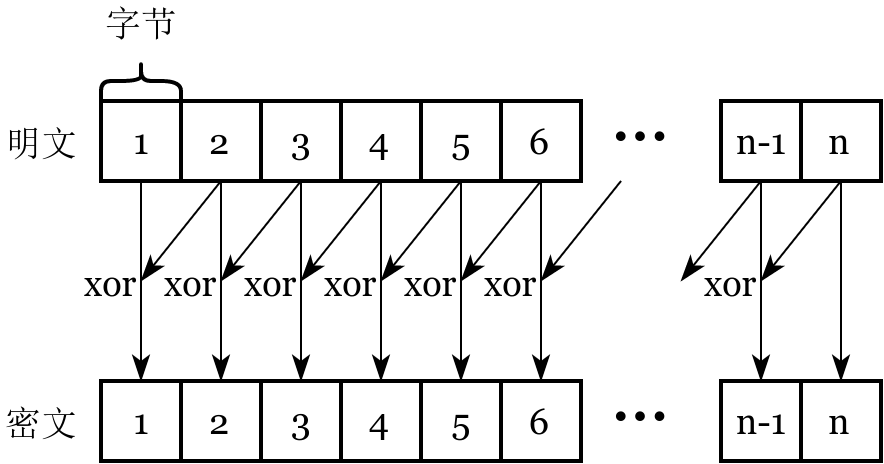
\includegraphics[width=0.8\linewidth]{res/homework_4/encrypt.png}
		\caption{数据加密方式}
		\label{fig:encrypt}
	\end{figure}

	\subsubsection{源程序}
	由于源程序较长,本部分的源程序见附录部分。(第\pageref{code:4_4}页)

	\subsubsection{实验步骤}
	\begin{enumerate}
		\item 对于实验三任务一中的源程序进行修改,在录入与显示部分对于数据进行加密与解密。
		\item 采用堆栈法和间接跳转法对于整个程序进行反跟踪处理。
		\item 对源程序进行编译和链接。若出现错误,对于整个程序进行修改并重新编译和链接。
		\item 对于源程序进行调试,确保反跟踪部分和加密部分有效。
		\item 重新对源程序进行编译和链接,此时\textbf{不生成调试信息},以增加反跟踪难度。
		\item 交付源程序。
	\end{enumerate}

	\subsubsection{实验记录与分析}
	\begin{enumerate}
		\item 实验环境条件:i7 3.6GHz,8G内存;Archlinux下DOSBox0.74; VIM.EXE 7.3; TASM 5.0、TLINK 5.0、TD 5.0编译、链接、调试套件。
		\item 首先按照设计思想中的加密方法对源程序追加加密部分,同时,将预存的数据按照此加密方法进行加密,并以密文的形式写入汇编文件中。
		\item 对于源程序进行编译、链接、调试,发现在运行过程中出现错误,具体原因为加密和解密算法不匹配。
		\item 重新对于文件进行编译和调试,最后达到如图\ref{fig:passwd}的效果,即当密码输入错误时程序直接退出。
			\begin{figure}[H]
				\centering
				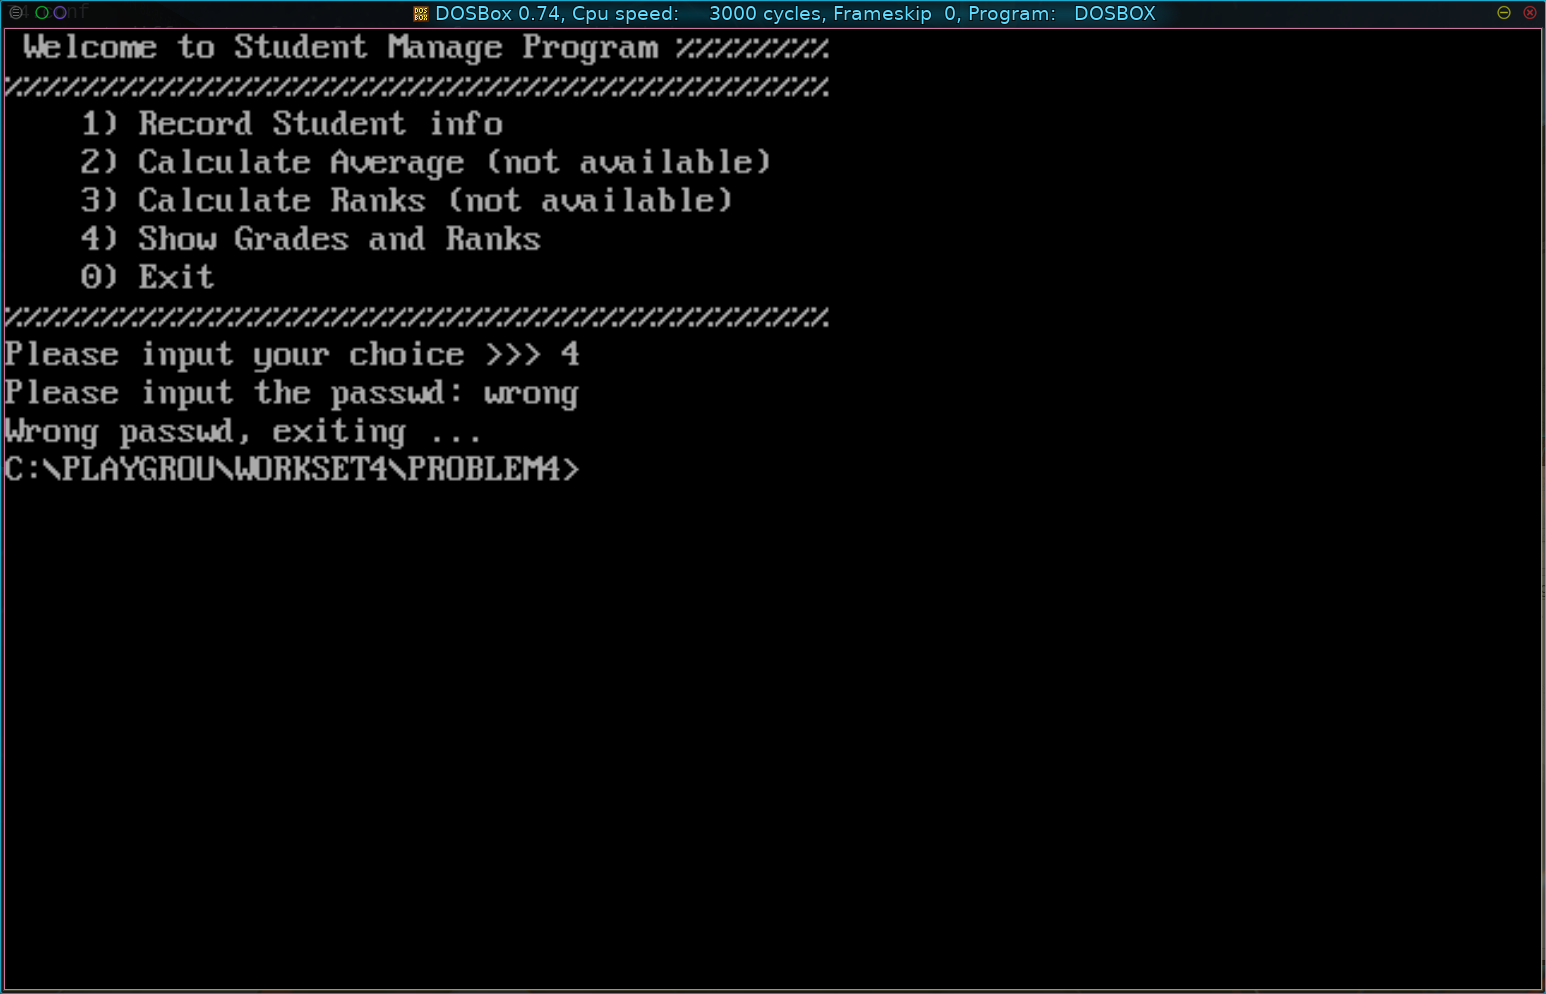
\includegraphics[width=0.85\linewidth]{res/homework_4/passwd.png}
				\caption{将程序的查找部分进行加密}
				\label{fig:passwd}
			\end{figure}
		\item 加密部分编写完成后,将源程序进行更改,追加反跟踪部分,并进行测试。
		\item 在对于反跟踪部分的编写过程中,出现了由于标号太远超出跳转范围的错误。将其改为远标号重新进行编译后即可正常运行。
		\item 对于程序进行调试,发现在堆栈检查的部分由于调试程序修改了堆栈,程序没有正常向下执行,而是跳转到了别的地方。说明堆栈检反跟踪是成功的。
		\item 重新对源程序进行编译,此时关闭调试信息开关(即在编译时仅使用TASM /z /zi进行编译,在链接时仅使用TLINK /3 /Tde进行链接)。
		\item 再次打开调试器,观察到所有的调试信息均已消失,如图\ref{fig:nodebug}所示,至此,程序处理完成,可以进行交付。
			\begin{figure}[H]
				\centering
				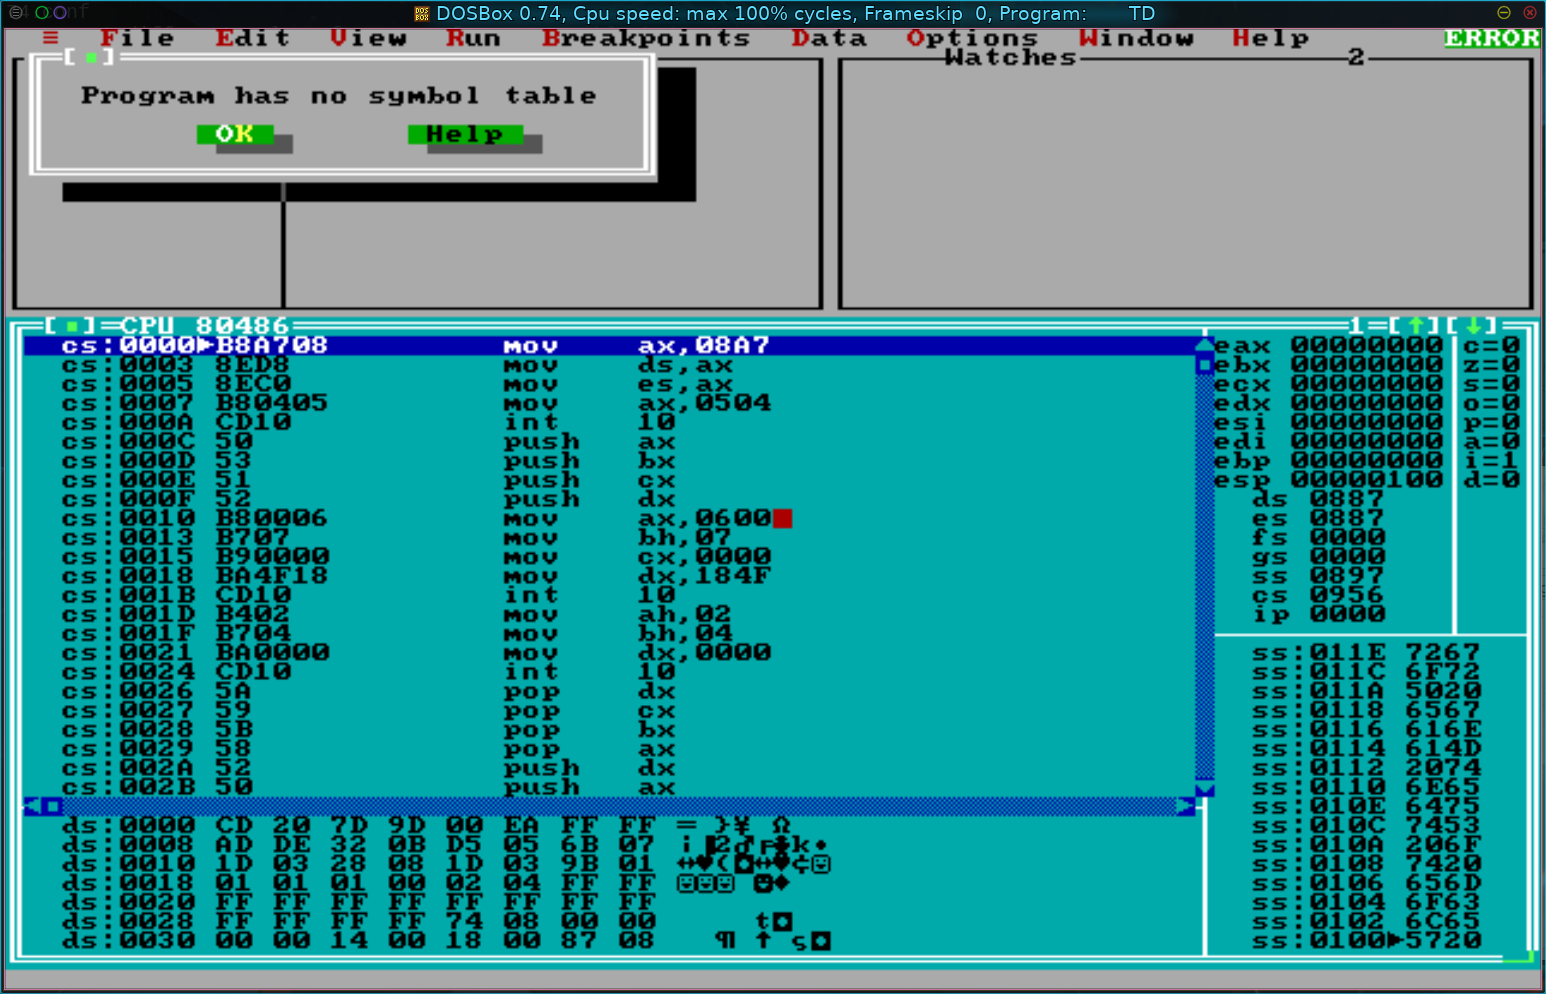
\includegraphics[width=0.85\linewidth]{res/homework_4/nodebug.png}
				\caption{除去调试信息后的调试界面}
				\label{fig:nodebug}
			\end{figure}
	\end{enumerate}

	\subsection{任务五}
	\subsubsection{实验思想}
	对于程序的破解,主要从以下几个方面进行:
	\begin{itemize}
		\item 直接运行程序,观察程序的输出以及程序的关键性位置,以找到破解的入口。
		\item 对于密码输入的位置应该重点观察,尝试直接读出加密的方式。
		\item 在成功获得密码之后直接运行程序,尝试直接从程序中获得所需要的信息,若不能获得所需要的信息,重新观察关键位置并破解。
		\item 对于反跟踪的部分需要首先识别出其位置,然后对其进行跳过。
	\end{itemize}

	\subsubsection{实验步骤}
	\begin{enumerate}
		\item 直接运行程序,观察程序输出以及请求密码的位置。
		\item \label{item:start}打开TD进行调试,跳转到密码请求的位置.任意输入一个密码,并观察程序的运行状态。
		\item \label{item:end}对于加密的部分进行进行选择性跳过。
		\item 重复\ref{item:start}到\ref{item:end}之间的步骤,直到所有的混淆性程序均已经被跳过为止。
		\item 根据所获得的加密算法推算出密码,或者直接取得数据。
		\item 直接运行程序,输入密码,并尝试获得数据字段。
		\item 若通过直接运行程序不能获得数据字段,重新调试并尝试从内存数据中推算出数据字段。
	\end{enumerate}

	\subsubsection{实验记录与分析}
	\begin{enumerate}
		\item 实验环境条件:i7 3.6GHz,8G内存;Archlinux下DOSBox0.74;使用TD5.0作为调试工具,xdotool作为自动化输入工具。
		\item 首先直接运行程序,发现要求输入密码。任意输入一个错误的密码,程序退出。过程如图\ref{fig:wrongpass}所示。
			\begin{figure}[H]
				\centering
				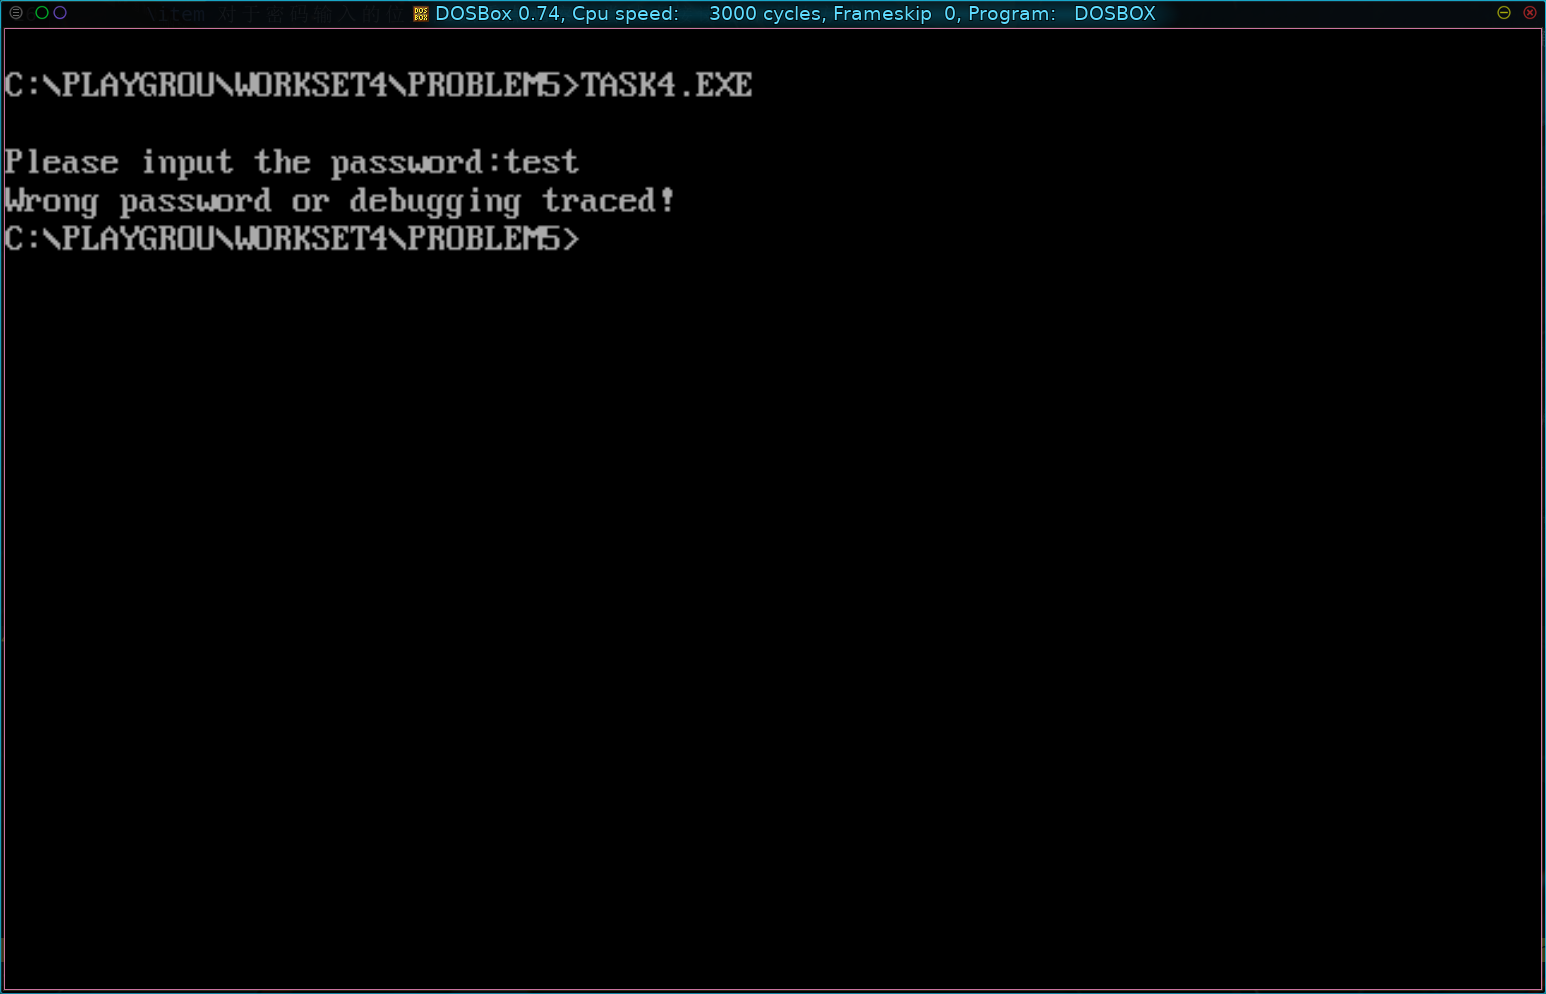
\includegraphics[width=0.85\linewidth]{res/homework_4/wrongpass.png}
				\caption{直接运行程序}
				\label{fig:wrongpass}
			\end{figure}
		\item 打开TD直接单步执行程序,发现在执行到特定语句后,程序直接跳转然后结束,对程序进行观察,发现之一部分的程序进行了时间检查,如图\ref{fig:timecheck}所示。
			\begin{figure}[H]
				\centering
				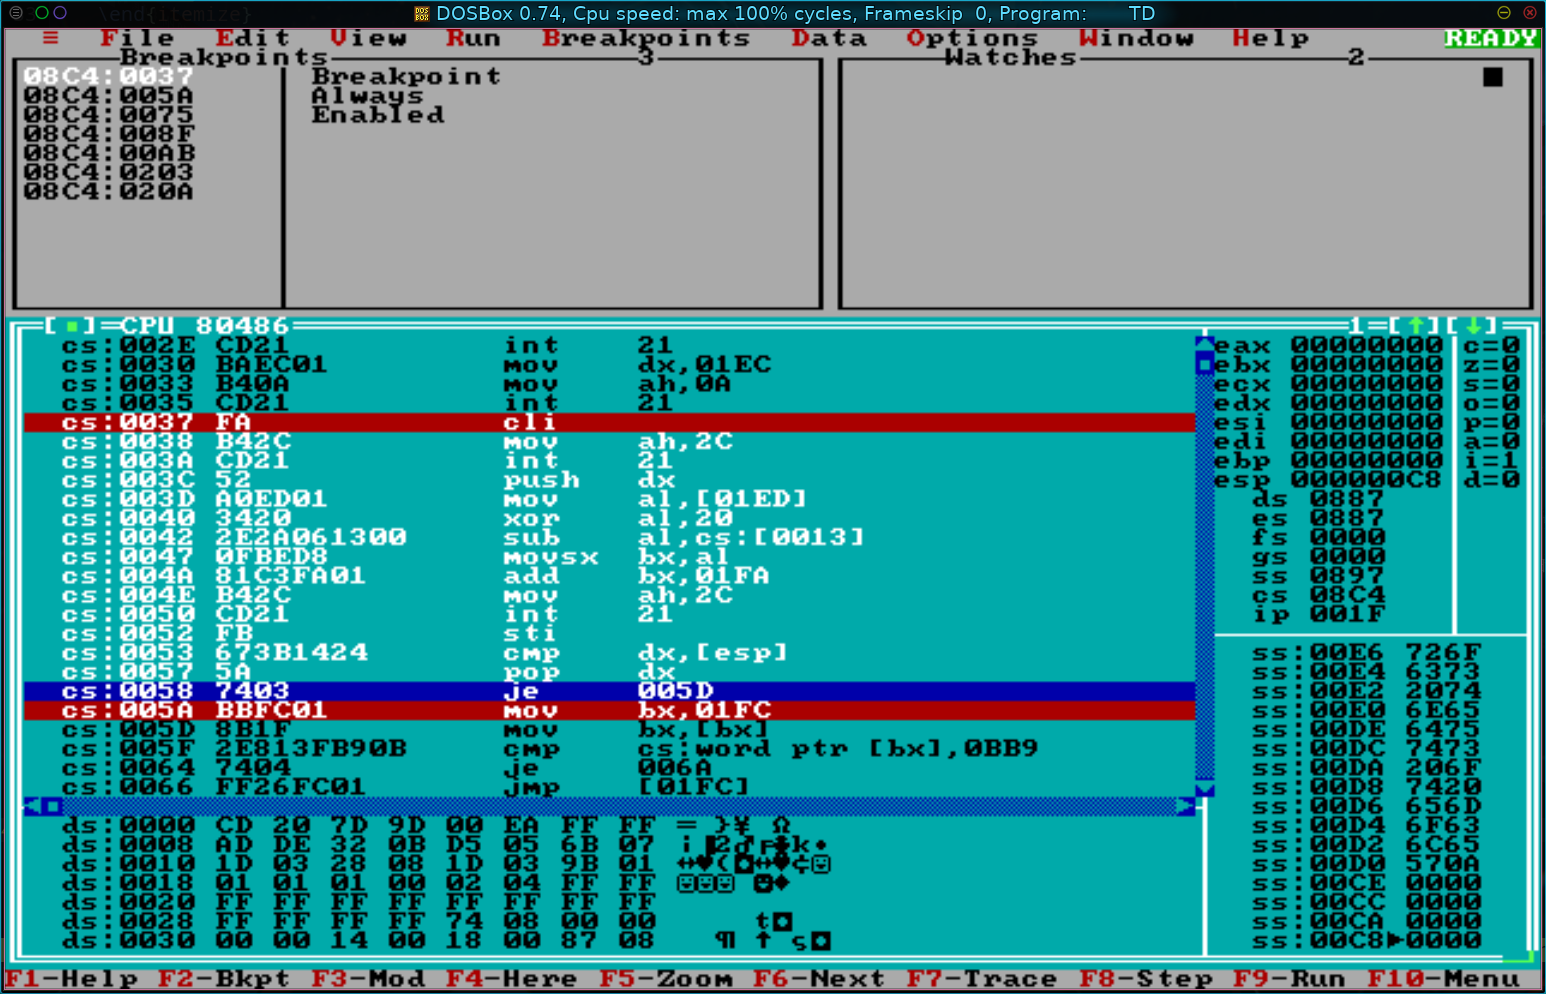
\includegraphics[width=0.85\linewidth]{res/homework_4/timecheck.png}
				\caption{时间检查部分的反汇编代码}
				\label{fig:timecheck}
			\end{figure}
		\item 跳过这些程序后继续执行,发现程序依然在执行某间接跳转后程序直接停止。
		\item 将上述两个步骤的代码用nop填充,并重新执行程序,将其他干扰性代码用nop填充,直到执行到显示主界面位置。显示主界面如图\ref{fig:mainUI}所示。发现有检查输入的姓名是否存在的功能。又已知姓名的格式为姓的全拼加上名的简拼,于是将`chenzh'字符串的所有大小写组合使用脚本进行自动输入测试,并观察检测所得的结果,发现最终的正确姓名为`ChenZh'。
			\begin{figure}[H]
				\centering
				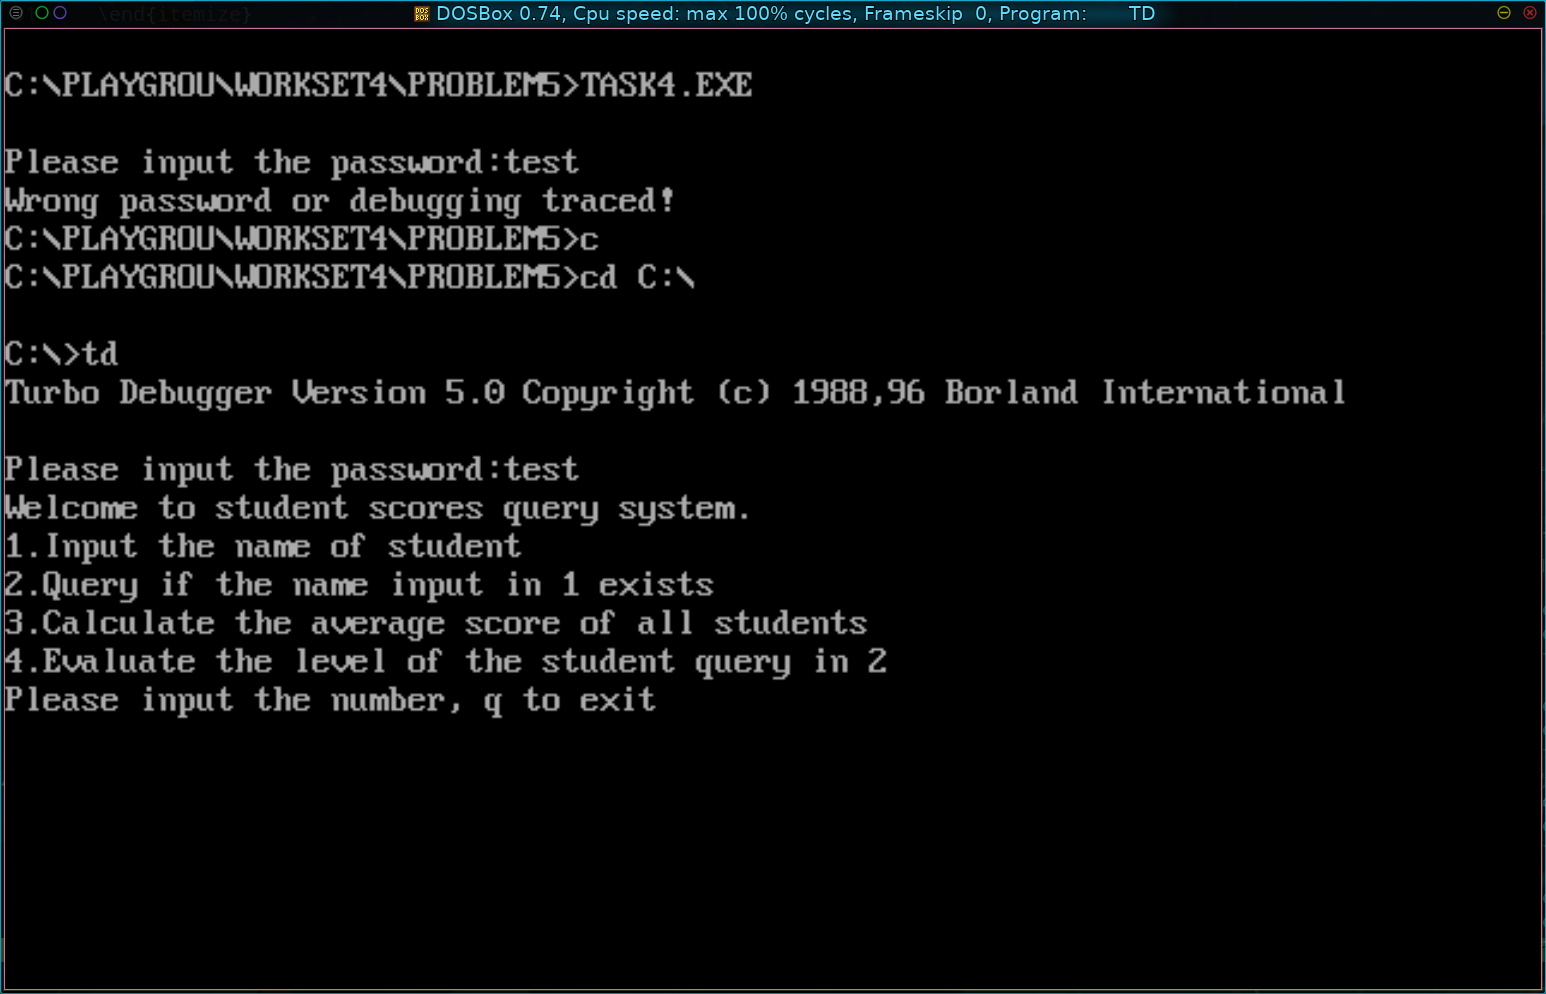
\includegraphics[width=0.85\linewidth]{res/homework_4/mainUI.png}
				\caption{跳过密码检查后的程序主界面}
				\label{fig:mainUI}
			\end{figure}
		\item 输入姓名后,得知其分数评价为A,但是依然不知道其平均分。对于计算分数评价的函数进行定位,加上断点后重新进行调试,单步执行并分析代码,获得分数评价算法后直接在计算的过程中从寄存器中读出其平均分为5AH,即90分,图\ref{fig:finalGrade}中bl字段即为其平均分,高亮的代码部分为进行分数评价的代码。
			\begin{figure}[H]
				\centering
				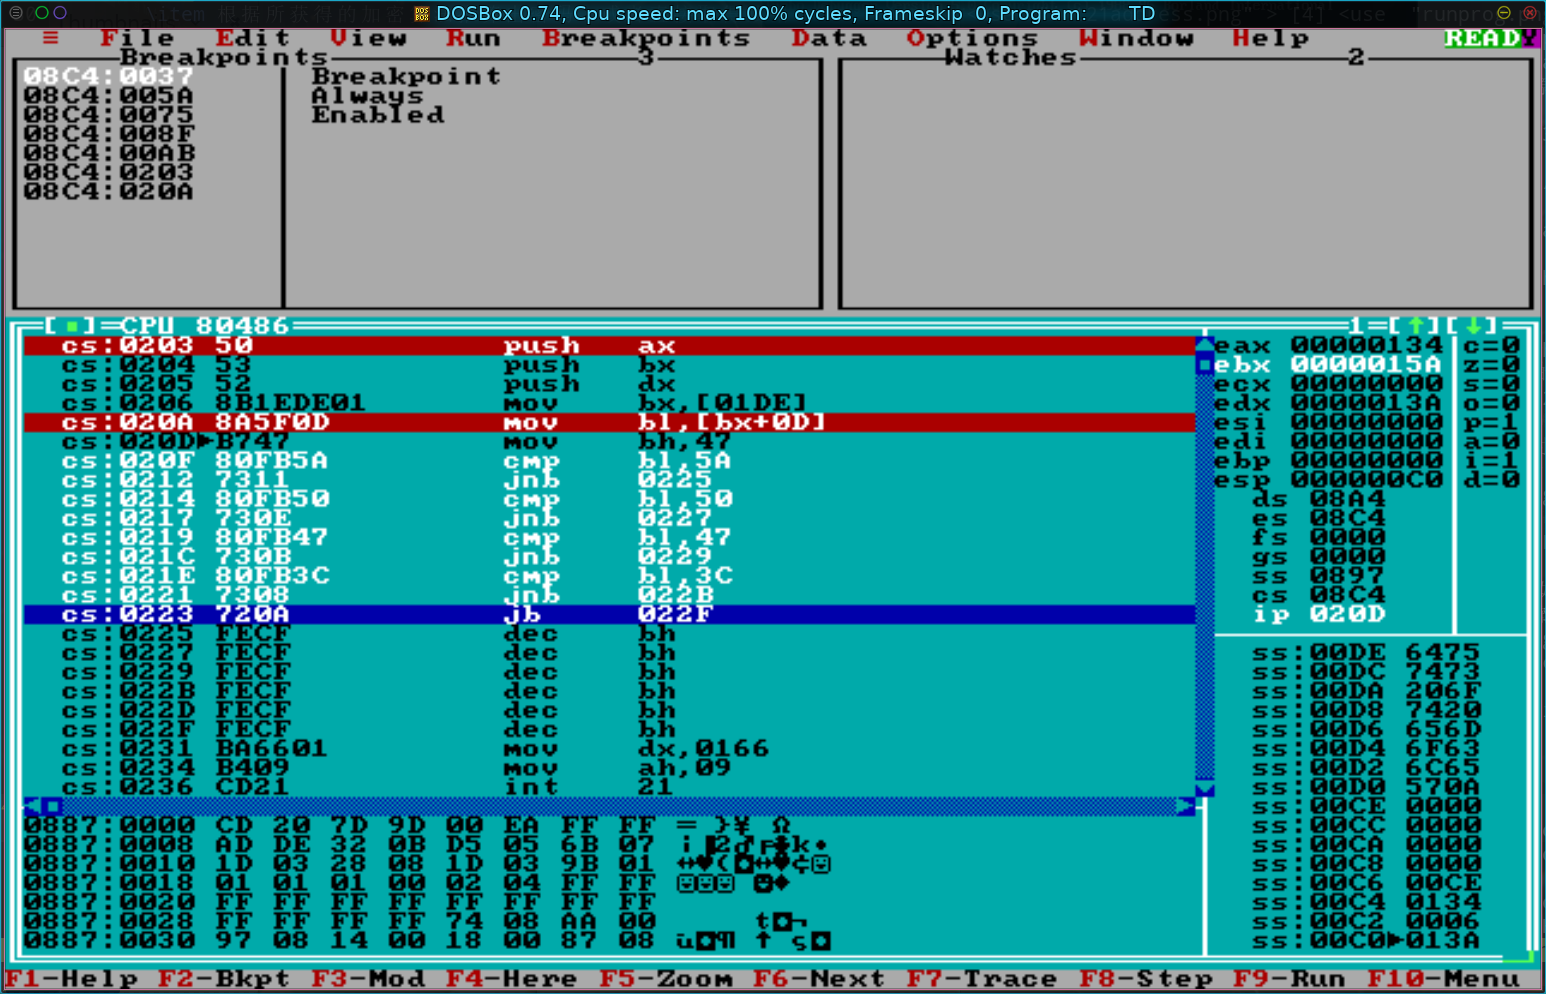
\includegraphics[width=0.85\linewidth]{res/homework_4/finalGrade.png}
				\caption{取得最终成绩}
				\label{fig:finalGrade}
			\end{figure}
	\end{enumerate}


	\section{总结与体会}
	通过这次实验,我对于汇编语言有了更为深刻的认识。在前三个实验中,我不见了解到汇编中断的工作原理以及对于硬件的读写操作,与此同时更是对于计算机低层工作原理的一次探索。在尝试获得中断地址时由于中断被TD接管而未能获得正确的地址,这也从另一个方面说明了dos系统中断的工作方式,同时,这也锻炼了我对于问题的排查以及纠正能力。\par
	在任务4(加密实验)中,我对于程序的加密和反跟踪方法有了初步的了解,并将之用于实践。同时我也了解到,反跟踪也是解释型语言相对于编译型语言所缺少的一项特性(由于解释型语言源码必须开放),这也是我对于各个商业软件的保全保护方式的一个初步探知。\par
	而在任务5(解密实验)中,我对于程序的加密与反跟踪有了更为深入的了解,并深刻的体会到了破解程序要难于加密程序。同时,对于解密方法的尝试也让我了解到如何加密才能使程序更为安全,更不易被破解,从而相辅相成的了解了程序的加密解密的原理和方法。


%% Part Five %%%%%%%%%%%%
%%%%%%%%%%%%%%%%%%%%%%%%%
\newpage
\part{WIN32编程}

	\section{实验目的与要求}
	\begin{enumerate}
		\item 熟悉WIN32程序的设计和调试方法;
		\item 熟悉宏汇编语言中INVOKE、结构变量、简化段定义等功能;
		\item 进一步理解机器语言、汇编语言、高级语言之间以及实方式、保护方式之间的一些关系。
	\end{enumerate}

	\section{实验内容}
	编写一个基于窗口的WIN32程序,实现学生成绩表信息的平均值计算及显示功能(借鉴前面实验中的一些做法),具体要求如下描述。\par
	功能一:编写一个基于窗口的WIN32程序的菜单框架,具有以下的下拉菜单项:\par
	\begin{tabular}{l | l | l}
		File & Action & Help \\ \midrule
		Exit & Average & About \\ \cmidrule{2-2}
		& List &
	\end{tabular}

	点菜单File下的Exit选项时结束程序;点菜单Help下的选项About,弹出一个消息框,显示本人信息,类似图\ref{fig:example0}所示。点菜单Action下的选项Average、List将分别实现计算平均值或显示所有成绩的功能(详见功能二的描述)。\par
	\begin{figure}[H]
		\centering
		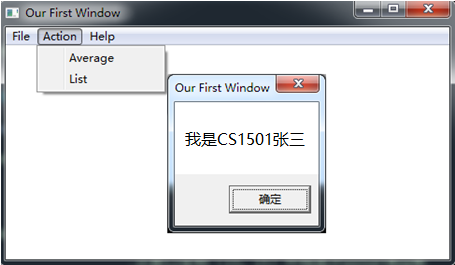
\includegraphics[width=0.7\linewidth]{res/homework_5/example0.png}
		\caption{菜单示例}
		\label{fig:example0}
	\end{figure}
	功能二:每个学生的相关信息包括:姓名(结尾含1个以上的数值0,共占10个字节),语文成绩(1个字节),数学成绩(1个字节),英语成绩(一个字节),平均成绩(1个字节),等级(1个字节)。要求采用结构变量存放学生的相关信息。学生人数至少5人。姓名和各科成绩直接在数据段中给定,不必运行时输入。成绩表中最后一个学生必须使用自己的姓名。\par
	\begin{enumerate}
		\item 点菜单项Average时,计算平均成绩并给出等级(等级的定义见实验一,但这里不用单独显示等级)。平均成绩的计算仍按照实验一的公式进行。平均成绩和等级保存到上述结构变量的相应字段中。用TD32观察计算结果。
		\item 点菜单项List时,要求能在窗口中列出所有学生信息,包括姓名、各科成绩、平均成绩、等级等。如图\ref{fig:example}所示。平均成绩尚未计算时,平均成绩及等级显示为空白。
			\begin{figure}[H]
				\centering
				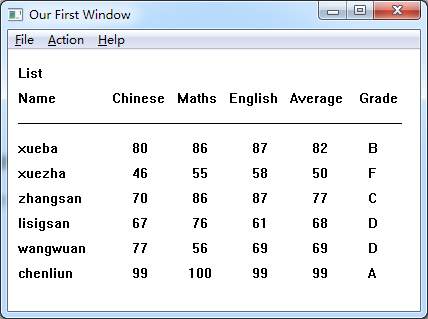
\includegraphics[width=0.7\linewidth]{res/homework_5/example.png}
				\caption{成绩单显示示意图}
				\label{fig:example}
			\end{figure}
	\end{enumerate}

	\section{实验过程}
	\subsection{设计思想}
	win32窗口程序与dos程序主要的不同在于其程序流程不同。win32程序对于输入的轮询由win32库代替用户完成,各个组件(句柄)之间使用信号进行通信,而用户主主要负责组件的构造以及信号的处理。除此之外,可以将数据使用STRUCT进行结构化存储,使用更为方便。此外,每一个句柄可将其视为一个对象,虽然各个函数没有被封装为类方法,但是整个程序依然采用了面向对象的设计思想。

	\subsection{模块图}
	图\ref{fig:modules}展示了程序的各个模块及其关系:\par
	\begin{figure}[H]
		\centering
		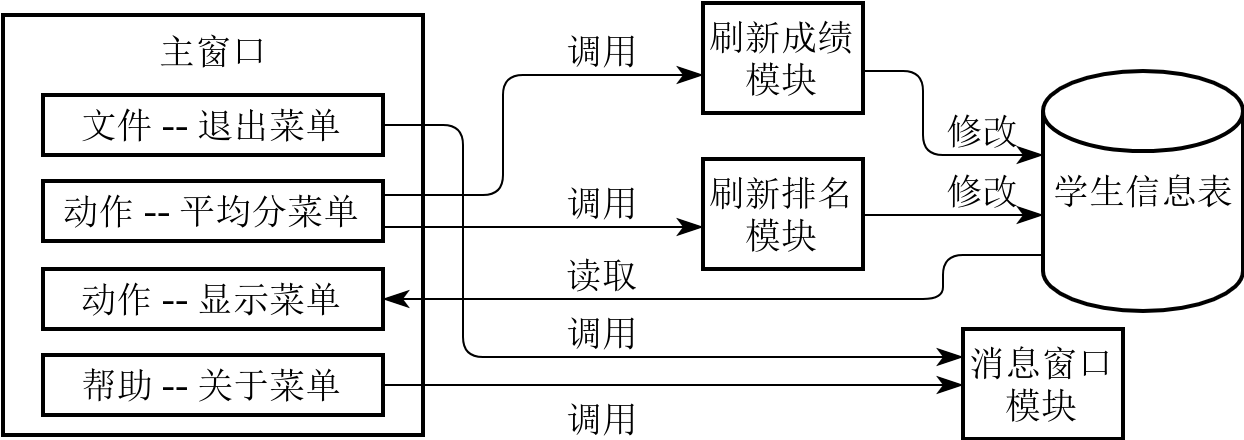
\includegraphics[width=0.85\linewidth]{res/homework_5/modules.png}
		\caption{程序模块图}
		\label{fig:modules}
	\end{figure}

	\subsection{实验步骤}
	\begin{enumerate}
		\item 按照设计思想编写源程序,然后进行编译、链接。
		\item 对于出现的错误定位其位置,改正后重新编译、链接,重复上述步骤直到没有错误出现。
		\item 直接运行程序,对程序进行测试。
		\item 打开OllyDbg对程序进行调试,观察程序的运行状况以及运行细节。
	\end{enumerate}

	\subsection{源程序}
	源程序MAIN.ASM, RES.RC详见附录部分(第\pageref{code:5_1}页)

	\subsection{实验记录与分析}
	\begin{enumerate}
		\item 实验环境条件:i7 3.6GHz,8G内存;Archlinux下Wine win32模拟器;使用OllyDbg.exe作为调试工具,ML.EXE作为编译工具,LINK.EXE作为链接工具,RC.EXE作为资源编译工具,NMAKE作为makefile处理工具。
		\item 按照设计思想编写源程序,然后对于源程序进行编译和链接,在编译和链接的过程中没有出现错误。
		\item 直接运行程序,选择Action\textrightarrow show/refresh list,程序正常显示,如图\ref{fig:firstShow}所示,对于未计算的平均分以及排名不予显示。
			\begin{figure}[H]
				\centering
				\includegraphics[width=0.85\linewidth]{res/homework_5/firstShow.png}
				\caption{直接运行程序}
				\label{fig:firstShow}
			\end{figure}
		\item 选择Action\textrightarrow refresh Average and Rank,出现提示信息后再次选择Action\textrightarrow show/refresh list,经过验证发现成绩与排名均计算正常,如图\ref{fig:secondShow}所示。
			\begin{figure}[H]
				\centering
				\includegraphics[width=0.85\linewidth]{res/homework_5/secondShow.png}
				\caption{刷新平均分和排名之后的显示}
				\label{fig:secondShow}
			\end{figure}
		\item 最后对于About和Exit进行测试,发现其均能正常运行。
		\item 打开OllyDbg,加载程序,发现其各个段地址均为32位,如图\ref{fig:dbg1}所示,而在对于一个函数进行invoke操作时,在反汇编长口中其实是以call的方式进行,但编译器会自动加上压栈与出栈命令来保护寄存器,参数的传递也由编译器自动完成。
			\begin{figure}[H]
				\centering
				\includegraphics[width=0.95\linewidth]{res/homework_5/dbg1.png}
				\caption{打开调试界面}
				\label{fig:dbg1}
			\end{figure}
		\item 在使用OllyDbg的过程中,发现结构化数据对于程序的编写提供了极大的便利,并且相较于TurboD ebugger此调试器可以显示更多有关于源代码的信息,包括函数名称,系统调用,以及堆栈中的参数信息等,使用更加方便。
	\end{enumerate}

	\section{总结与体会}
	通过本次试验,我对于汇编的了解更为深刻与广泛。我了解到汇编不仅仅限于较小的命令行程序的编写,同样可使用汇编较为容易的编写窗口程序,并使用win32汇编成功的将前几次的任务进行改写。此外,win32汇编中的各个特性(如结构的引入)使我更加清晰的看到了汇编与编译型高级语言之间的关系,更深入的了解到了高级语言在编译的过程中是怎样被翻译的。\par
	此外,我还了解到了几种反汇编win32程序的工具,如TD32,OllyDbg,IDA Pro等等,并尝试使用它们。在使用的过程中,TD32未能正确识别ML.EXE生成的符号表,因此转而使用OllyDbg进行调试,这使我对于反汇编工具的特性有了更深入的了解,在今后的学习过程中可以使用其对程序进行调试与优化。



%% Appendix %%%%%%%%%%%%%
%%%%%%%%%%%%%%%%%%%%%%%%%
\addtocontents{toc}{\protect\vspace{4em}}
\newpage
\appendix
\section{参考文献}
\begin{minipage}{1.0\textwidth}
	\begin{enumerate}[{[}1{]}]
		\item 元珍, 忠升, 宗芬. 80X86 汇编语言程序设计[M]. 华中科技大学出版社, 2005.
		\item Barry Wilks. DOS INT 21h - DOS Function Codes[EB/OL]. [2017-03-23]. http://spike.scu.edu.au/~barry/interrupts.html.
		\item Borland International. Turbo Debugger, Version 2.5: User's Guide. 1991.
		\item Barry Wilks. DOS INT 21h - DOS Function Codes[EB/OL]. [2017-03-23]. http://spike.scu.edu.au/~barry/interrupts.html.
		\item 汇编语言教学网站(http://115.156.187.251/huibian1/site/index.jsp)\textrightarrow 资料下载 \textrightarrow 案例 \textrightarrow win32程序、编译和连接。
		\item DOS Interrupts. (2017). Spike.scu.edu.au. Retrieved 4 May 2017, from http://spike.scu.edu.au/~barry/interrupts.html
		\item Embedded Systems/Mixed C and Assembly Programming - Wikibooks, open books for an open world. (2017). En.wikibooks.org. Retrieved 4 May 2017, from https://en.wikibooks.org/wiki/Embedded\_Systems/Mixed\_C\_and\_Assembly\_Programming
		\item Heng, C. (2017). Free Disassemblers, Decompilers, Hexadecimal viewers, Hex editors (thefreecountry.com). Thefreecountry.com. Retrieved 4 May 2017, from https://www.thefreecountry.com/programming/disassemblers.shtml
		\item Inline Assembly - OSDev Wiki. (2017). Wiki.osdev.org. Retrieved 4 May 2017, from http://wiki.osdev.org/Inline\_Assembly
		\item Mixing Assembly and C. (2017). Courses.engr.illinois.edu. Retrieved 4 May 2017, from https://courses.engr.illinois.edu/ece390/books/labmanual/c-prog-mixing.html
	\end{enumerate}
\end{minipage}

\flushleft
\newpage
\section{源代码}
\subsection{实验一}
\subsubsection{任务4}
\label{code:1_4}
\begin{codeFont}
	\lstinputlisting{res/homework_1/STUDENT.ASM}
\end{codeFont}

\newpage
\subsection{实验二}
\subsubsection{任务1}
\label{code:2_1}
	原程序见报告1,此处为修改后的程序。 \par
	{\emph{代码修改由命令`diff -u <old-file> <new-file>'生成,`+'表示增加的程序行,`-'表示删除的程序行,`@@ ... @@'表示修改的段落(新旧文件的行数),未显示部分为未修改部分}}
	\begin{codeFont}
		\lstinputlisting{res/homework_2/code1.ASM}
	\end{codeFont}
\newpage
\subsubsection{任务2}
\label{code:2_2}
	在任务一的基础上进行修改过后的源程序变更如下: \par
	{\emph{代码修改由命令`diff -u <old-file> <new-file>'生成,`+'表示增加的程序行,`-'表示删除的程序行,`@@ ... @@'表示修改的段落(新旧文件的行数),未显示部分为未修改部分}}
	\begin{codeFont}
		\lstinputlisting{res/homework_2/code2.ASM}
	\end{codeFont}
\newpage
\subsubsection{任务3}
\label{code:2_3}
	源代码分为3个部分:汇编部分,C程序部分以及由C程序生成的汇编部分。\par
	{\textbf{汇编部分:}} \par
	\begin{codeFont}
		\lstinputlisting{res/homework_2/code3_1.ASM}
	\end{codeFont}
	{\textbf{C程序部分:}} \par
	\begin{codeFont}
		\lstinputlisting[language=c]{res/homework_2/code3_2.C}
	\end{codeFont}
	{\textbf{生成汇编部分:}} \par
	\begin{codeFont}
		\lstinputlisting{res/homework_2/code3_3.ASM}
	\end{codeFont}

\newpage
\subsection{实验三}
\subsubsection{任务1}
\label{code:3_1}
	\noindent {\textbf{主程序 MAIN.ASM:}} \par
	\begin{codeFont}
		\lstinputlisting{res/homework_3/Problem1/MAIN.ASM}
	\end{codeFont}
	\noindent {\textbf{录入模块 SUBMOD1.ASM:}} \par
	\begin{codeFont}
		\lstinputlisting{res/homework_3/Problem1/SUBMOD1.ASM}
	\end{codeFont}
	\noindent {\textbf{平均分计算模块 SUBMOD2.ASM:}} \par
	\begin{codeFont}
		\lstinputlisting{res/homework_3/Problem1/SUBMOD2.ASM}
	\end{codeFont}
	\noindent {\textbf{排名计算模块 SUBMOD3.ASM:}} \par
	\begin{codeFont}
		\lstinputlisting{res/homework_3/Problem1/SUBMOD3.ASM}
	\end{codeFont}
	\noindent {\textbf{成绩单输出模块 SUBMOD4.ASM:}} \par
	\begin{codeFont}
		\lstinputlisting{res/homework_3/Problem1/SUBMOD4.ASM}
	\end{codeFont}
	\noindent {\textbf{宏库 MACROLIB:}} \par
	\begin{codeFont}
		\lstinputlisting{res/homework_3/Problem1/MACROLIB}
	\end{codeFont}
	\noindent {\textbf{工具函数库 COMMOD.ASM:}} \par
	\begin{codeFont}
		\lstinputlisting{res/homework_3/Problem1/COMMOD.ASM}
	\end{codeFont}
	\noindent {\textbf{nmake文件 MAKEFILE:}} \par
	\begin{codeFont}
		\lstinputlisting[language=sh]{res/homework_3/Problem1/MAKEFILE}
	\end{codeFont}
\newpage
\subsubsection{任务2}
\label{code:3_2}
	\noindent {\textbf{主程序 MAIN.C:}} \par
	\begin{codeFont}
		\lstinputlisting{res/homework_3/Problem2/MAIN.C}
	\end{codeFont}
	\noindent {\textbf{diff -u Problem1/SUBMOD1.ASM Problem2/SUBMOD1.ASM:}} \par
	\begin{codeFont}
		\lstinputlisting{res/homework_3/submod1.diff}
	\end{codeFont}
	\noindent {\textbf{diff -u Problem1/SUBMOD2.ASM Problem2/SUBMOD2.ASM:}} \par
	\begin{codeFont}
		\lstinputlisting{res/homework_3/submod2.diff}
	\end{codeFont}
	\noindent {\textbf{diff -u Problem1/SUBMOD3.ASM Problem2/SUBMOD3.ASM:}} \par
	\begin{codeFont}
		\lstinputlisting{res/homework_3/submod3.diff}
	\end{codeFont}
	\noindent {\textbf{diff -u Problem1/SUBMOD4.ASM Problem2/SUBMOD4.ASM:}} \par
	\begin{codeFont}
		\lstinputlisting{res/homework_3/submod4.diff}
	\end{codeFont}
	\noindent {\textbf{diff -u Problem1/COMMOD.ASM Problem2/COMMOD.ASM:}} \par
	\begin{codeFont}
		\lstinputlisting{res/homework_3/commod.diff}
	\end{codeFont}
	\noindent {\textbf{宏库 MACROLIB:}} \par
	\begin{codeFont}
		\lstinputlisting{res/homework_3/Problem2/MACROLIB}
	\end{codeFont}
	\noindent {\textbf{nmake文件 MAKEFILE:}} \par
	\begin{codeFont}
		\lstinputlisting[language=sh]{res/homework_3/Problem2/MAKEFILE}
	\end{codeFont}

\newpage
\subsection{实验四}
\subsubsection{任务1}
\label{code:4_1}
	\begin{codeFont}
		\lstinputlisting{res/homework_4/Problem1/GETADDR.ASM}
	\end{codeFont}
\newpage
\subsubsection{任务2}
\label{code:4_2}
	设置中断的程序:
	\begin{codeFont}
		\lstinputlisting{res/homework_4/Problem2/SETINT.ASM}
	\end{codeFont}
	恢复中断的程序
	\begin{codeFont}
		\lstinputlisting{res/homework_4/Problem2/REMOVE.ASM}
	\end{codeFont}
\newpage
\subsubsection{任务3}
\label{code:4_3}
	\begin{codeFont}
		\lstinputlisting{res/homework_4/Problem3/CMOS.ASM}
	\end{codeFont}
\newpage
\subsubsection{任务4}
\label{code:4_4}
	\noindent {\textbf{主程序 MAIN.ASM:}} \par
	\begin{codeFont}
		\lstinputlisting{res/homework_4/Problem4/MAIN.ASM}
	\end{codeFont}
	\noindent {\textbf{输入模块 SUBMOD1.ASM:}} \par
	\begin{codeFont}
		\lstinputlisting{res/homework_4/Problem4/SUBMOD1.ASM}
	\end{codeFont}
	\noindent {\textbf{平均分计算模块 SUBMOD2.ASM:}} \par
	\begin{codeFont}
		\lstinputlisting{res/homework_4/Problem4/SUBMOD2.ASM}
	\end{codeFont}
	\noindent {\textbf{排名计算模块 SUBMOD3.ASM:}} \par
	\begin{codeFont}
		\lstinputlisting{res/homework_4/Problem4/SUBMOD3.ASM}
	\end{codeFont}
	\noindent {\textbf{查询显示模块 SUBMOD4.ASM:}} \par
	\begin{codeFont}
		\lstinputlisting{res/homework_4/Problem4/SUBMOD4.ASM}
	\end{codeFont}
	\noindent {\textbf{宏库 MACROLIB:}} \par
	\begin{codeFont}
		\lstinputlisting{res/homework_4/Problem4/MACROLIB}
	\end{codeFont}
	\noindent {\textbf{nmake文件 MAKEFILE:}} \par
	\begin{codeFont}
		\lstinputlisting[language=sh]{res/homework_4/Problem4/MAKEFILE}
	\end{codeFont}
\newpage
\subsection{任务五}
\label{code:5_1}
	\noindent {\textbf{主程序 MAIN.ASM}}
	\begin{codeFont}
		\lstinputlisting{res/homework_5/MAIN.ASM}
	\end{codeFont}
	\noindent {\textbf{资源文件 res.rc}}
	\begin{codeFont}
		\lstinputlisting{res/homework_5/res.rc}
	\end{codeFont}



\end{document}
